 %_____________________________________________________________________________
%=============================================================================
% main.tex v6 (10-11-2013) \ldots dibuat oleh Lionov - Informatika FTIS UNPAR
% 
% Ini adalah file utama (main.tex), berisi perintah-perintah yang khusus 
% dibuat untuk template ini
%
% 			JANGAN MENGUBAH APAPUN DI DALAM FILE INI,
%			KECUALI ANDA TAHU APA YANG ANDA LAKUKAN !!!
%
% Jika ada tambahan perintah, dapat anda tuliskan di tempat yang telah disediakan 
% di baris 295 pada file ini
% Jika daftar tabel tidak digunakan, anda harus menghapus (beri komentar) secara
% manual di baris 470
%
% Bug, kritik, saran: silahkan kirimkan via email ke lionov@unpar.ac.id
%
% Perubahan pada versi 6 (10-11-2013):
%	- perbaikan pada abstract dengan paragraf lebih dari satu: perbaikan vertical spacing
%	- perbaikan pada tampilan bab dan lampiran: tidak perlu menuliskan apapun untuk 
%	  menampilkan semuanya (di data.tex) atau -1 jika tidak ada lampiran
%	- halaman bernomor genap untuk halaman romawi sudah dimunculkan
%	- Kurikulum 2013 : perubahan nama buku skripsi 
%
% Perubahan dari versi sebelumnya :
%	versi 5 (21-10-2012)
%	- halaman terakhir setiap bab tidak ada headernya jika kosong
%	versi 4 (06-08-2012)
% 	- penggabungan main.tex, depan.tex dan setup.tex menjadi main.tex
% 	- menambahkan keterangan di lampiran untuk kode program 
% 	- ukuran font dapat diubah langsung di tiap lampiran
% 	versi 3 (09-07-2012): 
%	- Tidak ada di file ini
% 	versi 2 :
% 	- "Daftar Referensi" tidak perlu diubah secara manual (tidak perlu mengubah file bahasai.ldf)
% 	- Bahasa Indonesia dari abstract adalah abstrak (secara otomatis), bukan ringkasan
% 	- Spasi pada buku dokumen final adalah onehalfspacing
%
% to do : - hilangkan secara otomatis daftar tabel/gambar jika tidak digunakan
%         - (IT) aturan penulisan algoritma untuk IT (pakai algo.sty ?)
%=============================================================================

%=============================================================================
% setup.tex v2 (08-07-2012)
% Perubahan pada versi 2:
% - Menambahkan perintah untuk judulINA dan judulENG
% - Menghapus \usepackage{microtype}, yang pada beberapa kasus menjadi masalah
%=============================================================================
% depan.tex v2 (09-07-2012)
% Perubahan pada versi 2:
% - Menambahkan halaman depan dalam bahasa inggris
%=============================================================================

%setup.tex
\documentclass[11pt,a4paper,twoside,openright,notitlepage]{report} 

\usepackage[bahasa]{babel} %bahasa indonesia
\usepackage[T1]{fontenc}  %encoding
% \usepackage{mathptmx}
% \usepackage{venturisold}
% \usepackage{helvet}
% \usepackage{fouriernc} 
\usepackage{abstract} %manipulasi abstract
\usepackage{chappg} % format daftar isi 
\usepackage{color} %warna
\usepackage{etoolbox} %untuk programming if-then
\usepackage{fancyhdr} %format header & footer
\usepackage{float} %penempatan gambar di tempat yg seharusnya
\usepackage[inner=2.5cm,outer=2cm,top=2.5cm,bottom=2.5cm]{geometry} %margin
\usepackage{graphicx} %gambar
\usepackage{listings} %source code
\usepackage{lscape} %landscape untuk source code
\usepackage{multicol} %multiple column
\usepackage{ifthen} % if then
\usepackage[pagewise]{lineno} %line numbering
\usepackage{lipsum} % untuk testing
\usepackage{titlesec} %judul header
\usepackage{tocbibind} %daftar isi, gambar, tabel dll
\usepackage{tocloft} % format daftar isi 
\usepackage{setspace} %line spacing
\usepackage{xstring} %manipulasi string
\usepackage[plainpages=false,pdfpagelabels,unicode]{hyperref} %\autoref, \phantomsection & link 

\usepackage{emptypage}

\let\abstractname\Abstrak

\titleformat{\chapter}[display] {\Large\bfseries\centering}{\MakeUppercase{\chaptertitlename} \thechapter}{15pt}{\Large\MakeUppercase}

\renewcommand{\cftchapfont}{\scshape \bfseries}

\renewcommand{\cfttoctitlefont}{\hfil\Large\bfseries\MakeUppercase}
\renewcommand{\cftaftertoctitle}{\hfill}
\renewcommand{\cftloftitlefont}{\hfill\Large\bfseries\MakeUppercase}
\renewcommand{\cftafterloftitle}{\hfill}
\renewcommand{\cftlottitlefont}{\hfill\Large\bfseries\MakeUppercase}
\renewcommand{\cftafterlottitle}{\hfill}

% Tidak perlu ada kata "Bab", "Gambar" atau "Tabel" di daftar 
% \renewcommand{\cftchappresnum}{{\bf \scshape Bab} } 
% \renewcommand{\cftchapnumwidth}{1.5cm}
% \renewcommand{\cftfigpresnum}{{Gambar\ }} 
% \renewcommand{\cftfignumwidth}{2.5cm}
% \renewcommand{\cfttabpresnum}{{Tabel\ }} 
% \renewcommand{\cfttabnumwidth}{2cm}

\newcommand{\apptoc}{
	% Hapus kata "Lampiran" dari daftar isi
	%\addtocontents{toc}{\protect\renewcommand{\protect\cftchappresnum}{\bf \scshape Lampiran\  }}%
	%\addtocontents{toc}{\protect\renewcommand{\protect\cftchapnumwidth}{2.75cm}}
	\addtocontents{toc}{\protect\renewcommand{\protect\cftchappresnum}{\bf \scshape}}%	

}

\newcommand{\vnama}{Jane Doe}
\newcommand{\vlnama}{John Doe}
\newcommand{\vnpm}{1992700001}
\newcommand{\vprodiINA}{SAINS}
\newcommand{\vprodiENG}{SCIENCE}
\newcommand{\vstaINA}{UJIAN}
\newcommand{\vstaENG}{EXAM}
%\newcommand{\vjudul}{Judul Skripsi/Tugas Akhir}
\newcommand{\vpembu}{Plato}
\newcommand{\vpembs}{Euclid}
\newcommand{\vpengi}{Plato}
\newcommand{\vpengii}{Euclid}
\newcommand{\vtanggal}{1}
\newcommand{\vbulan}{Januari}
\newcommand{\vtahun}{1970}
\newcommand{\vmode}{final}
\newcommand{\vspacing}{double}
\newcommand{\vlineno}{yes}
\newcommand{\vkunciina}{Skripsi, Tugas Akhir}
\newcommand{\vkuncieng}{Undergraduate Thesis, Final Project}
\newcommand{\vkajur}{Jack Doe}
\newcommand{\vkajurmat}{Jack Doe}
\newcommand{\vkajurfis}{Jack Doe}
\newcommand{\vkajurtif}{Jack Doe}

\newcommand{\namanpm}[2]{
	\renewcommand{\vnama}{\uppercase{#1}} \renewcommand{\vlnama}{#1} \hypersetup{pdfauthor={#2 - #1}}
	\renewcommand{\vnpm}{#2} \hypersetup{pdfcreator={#2}} \StrChar{\vnpm}{6}[\vprodiN]
	\ifdefstring{\vprodiN}{1}{
		\renewcommand{\vprodiINA}{MATEMATIKA} \renewcommand{\vprodiENG}{MATHEMATICS} 
		\renewcommand{\vstaINA}{SKRIPSI} \renewcommand{\vstaENG}{FINAL PROJECT} \renewcommand{\vkajur}{\vkajurmat}}{}
	\ifdefstring{\vprodiN}{2}{
		\renewcommand{\vprodiINA}{FISIKA} \renewcommand{\vprodiENG}{PHYSICS} 
		\renewcommand{\vstaINA}{TUGAS AKHIR} \renewcommand{\vstaENG}{FINAL PROJECT} \renewcommand{\vkajur}{\vkajurfis}}{}
	\ifdefstring{\vprodiN}{3}{
		\renewcommand{\vprodiINA}{TEKNIK INFORMATIKA} \renewcommand{\vprodiENG}{INFORMATICS} 
		\renewcommand{\vstaINA}{SKRIPSI} \renewcommand{\vstaENG}{UNDERGRADUATE THESIS} \renewcommand{\vkajur}{\vkajurtif}}{}}

%\newcommand{\judul}[1]{\renewcommand{\vjudul}{\uppercase{#1}}\hypersetup{pdftitle={#1}, pdfsubject={#1}}}
\newcommand{\pembimbing}[2]{\renewcommand{\vpembu}{#1}\renewcommand{\vpembs}{#2}}
\newcommand{\penguji}[2]{\renewcommand{\vpengi}{#1}\renewcommand{\vpengii}{#2}}
\newcommand{\kajur}[3]{\renewcommand{\vkajurmat}{#1}\renewcommand{\vkajurfis}{#2}\renewcommand{\vkajurtif}{#3}}
\newcommand{\tanggal}[3]{\renewcommand{\vtanggal}{#1}\renewcommand{\vtahun}{#3}
	\newcommand{\vcbulan}{#2}
	\ifdefstring{\vcbulan}{1}{\renewcommand{\vbulan}{Januari}}{}
	\ifdefstring{\vcbulan}{2}{\renewcommand{\vbulan}{Februari}}{}
	\ifdefstring{\vcbulan}{3}{\renewcommand{\vbulan}{Maret}}{}
	\ifdefstring{\vcbulan}{4}{\renewcommand{\vbulan}{April}}{}
	\ifdefstring{\vcbulan}{5}{\renewcommand{\vbulan}{Mei}}{}
	\ifdefstring{\vcbulan}{6}{\renewcommand{\vbulan}{Juni}}{}
	\ifdefstring{\vcbulan}{7}{\renewcommand{\vbulan}{Juli}}{}
	\ifdefstring{\vcbulan}{8}{\renewcommand{\vbulan}{Agustus}}{}
	\ifdefstring{\vcbulan}{9}{\renewcommand{\vbulan}{September}}{}
	\ifdefstring{\vcbulan}{10}{\renewcommand{\vbulan}{Oktober}}{}
	\ifdefstring{\vcbulan}{11}{\renewcommand{\vbulan}{November}}{}
	\ifdefstring{\vcbulan}{12}{\renewcommand{\vbulan}{Desember}}{}	
}

\newcommand{\judulINA}[1]{\newcommand{\vjudulINA}{\uppercase{#1}}\hypersetup{pdftitle={#1},pdfsubject={#1}}}
\newcommand{\judulENG}[1]{\newcommand{\vjudulENG}{\uppercase{#1}}\hypersetup{pdftitle={#1},pdfsubject={#1}}}
\newcommand{\abstrakINA}[1]{\newcommand{\vabstrakina}{#1}}
\newcommand{\abstrakENG}[1]{\newcommand{\vabstrakeng}{#1}}
\newcommand{\kunciINA}[1]{\renewcommand{\vkunciina}{#1} \hypersetup{pdfkeywords={#1}}}
\newcommand{\kunciENG}[1]{\renewcommand{\vkuncieng}{#1}}
\newcommand{\untuk}[1]{\newcommand{\vuntuk}{#1}}
\newcommand{\prakata}[1]{\newcommand{\vprakata}{#1}}
\newcommand{\mode}[1]{\renewcommand{\vmode}{#1}}
\newcommand{\linespacing}[1]{\renewcommand{\vspacing}{#1}}
\newcommand{\linenumber}[1]{\renewcommand{\vlineno}{#1}}

\newcommand{\bab}[1]{\newcommand{\vbab}{#1}}
\newcommand{\lampiran}[1]{\renewcommand{\vlmp}{#1}}

\newcommand{\vpilbab}{0}
\newcommand{\vbaba}{0}\newcommand{\vbabb}{0}\newcommand{\vbabc}{0}
\newcommand{\vbabd}{0}\newcommand{\vbabe}{0}\newcommand{\vbabf}{0}
\newcommand{\vbabg}{0}\newcommand{\vbabh}{0}\newcommand{\vbabi}{0}
\newcommand{\vpillmp}{0}
\newcommand{\vlmpa}{0}\newcommand{\vlmpb}{0}\newcommand{\vlmpc}{0}
\newcommand{\vlmpd}{0}\newcommand{\vlmpe}{0}\newcommand{\vlmpf}{0}
\newcommand{\vlmpg}{0}\newcommand{\vlmph}{0}\newcommand{\vlmpi}{0}
\newcommand{\vlmp}{x}

%	\ifdefempty{#1}{\bab{1,2,3,4,5,6,7,8,9} \tampilbab{\vbab}}{
\newcommand{\tampilbab}[1]{
	\ifdefempty{#1}{
		\renewcommand{\vbaba}{1}\renewcommand{\vbabb}{1}\renewcommand{\vbabc}{1}
		\renewcommand{\vbabd}{1}\renewcommand{\vbabe}{1}\renewcommand{\vbabf}{1}
		\renewcommand{\vbabg}{1}\renewcommand{\vbabh}{1}\renewcommand{\vbabi}{1}}{
	\renewcommand{\do}[1]{
		\renewcommand{\vpilbab}{##1}
		\ifdefstring{\vpilbab}{1}{\renewcommand{\vbaba}{1}}{}
		\ifdefstring{\vpilbab}{2}{\renewcommand{\vbabb}{1}}{}
		\ifdefstring{\vpilbab}{3}{\renewcommand{\vbabc}{1}}{}
		\ifdefstring{\vpilbab}{4}{\renewcommand{\vbabd}{1}}{}
		\ifdefstring{\vpilbab}{5}{\renewcommand{\vbabe}{1}}{}
		\ifdefstring{\vpilbab}{6}{\renewcommand{\vbabf}{1}}{}
		\ifdefstring{\vpilbab}{7}{\renewcommand{\vbabg}{1}}{}
		\ifdefstring{\vpilbab}{8}{\renewcommand{\vbabh}{1}}{}
		\ifdefstring{\vpilbab}{9}{\renewcommand{\vbabi}{1}}{}
	}
	\expandafter\docsvlist\expandafter{#1}
	}
}

\newcommand{\tampillmp}[1]{
	\ifdefempty{#1}{
		\renewcommand{\vlmpa}{1}\renewcommand{\vlmpb}{1}\renewcommand{\vlmpc}{1}
		\renewcommand{\vlmpd}{1}\renewcommand{\vlmpe}{1}\renewcommand{\vlmpf}{1}
		\renewcommand{\vlmpg}{1}\renewcommand{\vlmph}{1}\renewcommand{\vlmpi}{1}}{
	\ifdefstring{#1}{-1}{ }{
		\renewcommand{\do}[1]{ 
			\renewcommand{\vpillmp}{##1}
			\ifdefstring{\vpillmp}{A}{\renewcommand{\vlmpa}{1}}{}
			\ifdefstring{\vpillmp}{B}{\renewcommand{\vlmpb}{1}}{}
			\ifdefstring{\vpillmp}{C}{\renewcommand{\vlmpc}{1}}{}
			\ifdefstring{\vpillmp}{D}{\renewcommand{\vlmpd}{1}}{}
			\ifdefstring{\vpillmp}{E}{\renewcommand{\vlmpe}{1}}{}
			\ifdefstring{\vpillmp}{F}{\renewcommand{\vlmpf}{1}}{}
			\ifdefstring{\vpillmp}{G}{\renewcommand{\vlmpg}{1}}{}
			\ifdefstring{\vpillmp}{H}{\renewcommand{\vlmph}{1}}{}
			\ifdefstring{\vpillmp}{I}{\renewcommand{\vlmpi}{1}}{}}
		}
	\expandafter\docsvlist\expandafter{#1}
	}
}

\newcommand{\appspacing}{
	\ifdefstring{\vspacing}{single}{\singlespacing}{}
	\ifdefstring{\vspacing}{onehalf}{\onehalfspacing}{}
	\ifdefstring{\vspacing}{double}{\doublespacing}{}
	\ifdefstring{\vmode}{final}{\onehalfspacing}{}
}

\newcommand{\appline}{
	\ifdefstring{\vmode}{final}{\renewcommand{\vlineno}{no}}{}
	\ifdefstring{\vlineno}{yes}{\linenumbers \def\linenumberfont{\normalfont\tiny\sffamily}}{}
	\ifdefstring{\vlineno}{no}{\lstset{numbers=left, stepnumber=1, numbersep=5pt}}{}
	
}

\newcommand{\appmargin}{
	\ifdefstring{\vmode}{final}{}{\newgeometry{inner=3cm,outer=2.75cm,top=2cm,bottom=2cm}}
}

\renewcommand{\abstractnamefont}{\bf \MakeUppercase}

\makeatletter
\def\headrule{{%
  \if@fancyplain\let\headrulewidth\plainheadrulewidth\fi
  \hrule\@height\footrulewidth\@width\headwidth\vskip2pt%
  \hrule\@height\headrulewidth\@width\headwidth\vskip-\headrulewidth\vskip-4pt
}}
\def\footrule{}

\def\cleardoublepage{
	\clearpage
	\if@twoside \ifodd\c@page
	\else
		\hbox{}
		\vspace{\fill}
		\thispagestyle{empty}
		\newpage
	\if@twocolumn\hbox{}\newpage\fi\fi\fi}
\makeatother

\renewcommand{\headrulewidth}{1.25pt}
\renewcommand{\footrulewidth}{0.25pt}

\setlength{\headheight}{15pt}
\fancyhead[LE,RO]{\thepage}
\fancyhead[RE]{\small{\textsc{\nouppercase{\leftmark}}}}
\fancyhead[LO]{\small{\textsc{\nouppercase{\rightmark}}}}
\fancyfoot{}

\hypersetup{unicode=true,colorlinks=true,linkcolor=blue,citecolor=green,filecolor=magenta, urlcolor=cyan}

\lstset{basicstyle=\tiny, commentstyle=\color{blue}}
\lstset{frame=leftline, tabsize=4, breaklines=true}

%=============================================================================

%tambahkan perintah yang anda butuhkan di sini :

%=============================================================================
%end setup.tex

%_____________________________________________________________________________
%=============================================================================
% data.tex v5 (10-11-2013) \ldots dibuat oleh Lionov - Informatika FTIS UNPAR
%
% Perubahan pada versi 5 (10-11-2013)
% - Perbaikan pada memasukkan bab : tidak perlu menuliskan apapun untuk 
%	memasukkan seluruh bab (bagian V)
% - Perbaikan pada memasukkan lampiran : tidak perlu menuliskan apapun untuk
%	memasukkan seluruh lampiran atau -1 jika tidak memasukkan apapun
%
% Perubahan pada versi sebelumnya
%	versi 4 (21-10-2012)
%	- Data dosen dipindah ke dosen.tex agar jika ada perubahan/update data dosen
%   mahasiswa tidak perlu mengubah data.tex
%	- Perubahan pada keterangan dosen	
% 	versi 3 (06-08-2012)
% 	- Perubahan pada beberapa keterangan 
% 	versi 2 (09-07-2012):
% 	- Menambahkan data judul dalam bahasa inggris
% 	- Membuat bagian khusus untuk judul (bagian VIII)
% 	- Perbaikan pada gelar dosen
%_____________________________________________________________________________
%=============================================================================
% 								BAGIAN -
%=============================================================================
% Ini adalah file data (data.tex)
% Masukkan ke dalam file ini, data-data yang diperlukan oleh template ini
% Cara memasukkan data dijelaskan di setiap bagian
% Data yang WAJIB dan HARUS diisi dengan baik dan benar adalah SELURUHNYA !!
%=============================================================================
%_____________________________________________________________________________
%=============================================================================
% 								BAGIAN I
%=============================================================================
% Tambahkan package2 lain yang anda butuhkan di sini
%=============================================================================
\usepackage{booktabs}
\usepackage[table]{xcolor}
\usepackage{longtable}
\usepackage{amsmath}
%=============================================================================

%_____________________________________________________________________________
%=============================================================================
% 								BAGIAN II
%=============================================================================
% Mode dokumen: menetukan halaman depan dari dokumen, apakah harus mengandung 
% prakata/pernyataan/abstrak dll (termasuk daftar gambar/tabel/isi) ?
% - kosong : tidak ada halaman depan sama sekali (untuk dokumen yang 
%            dipergunakan pada proses bimbingan)
% - cover : cover saja tanpa daftar isi, gambar dan tabel
% - sidang : cover, daftar isi, gambar, tabel (IT: UTS-UAS Seminar 
%			 dan UTS TA)
% - sidang_akhir : mode sidang + abstrak + abstract
% - final : seluruh halaman awal dokumen (untuk cetak final)
% Jika tidak ingin mencetak daftar tabel/gambar (misalkan karena tidak ada 
% isinya), edit manual di baris 439 dan 440 pada file main.tex
%=============================================================================
% \mode{kosong}
% \mode{cover}
% \mode{sidang}
 \mode{sidang_akhir}
%\mode{final} 
%=============================================================================

%_____________________________________________________________________________
%=============================================================================
% 								BAGIAN III
%=============================================================================
% Line numbering: penomoran setiap baris, otomatis di-reset setiap berganti
% halaman
% - yes: setiap baris diberi nomor
% - no : baris tidak diberi nomor, otomatis untuk mode final
%=============================================================================
\linenumber{yes}
%=============================================================================

%_____________________________________________________________________________
%=============================================================================
% 								BAGIAN IV
%=============================================================================
% Linespacing: jarak antara baris 
% - single: opsi yang disediakan untuk bimbingan, jika pembimbing tidak
%            keberatan (untuk menghemat kertas)
% - onehalf: default dan wajib (dan otomatis) jika ingin mencetak dokumen
%            final/untuk sidang.
% - double : jarak yang lebih lebar lagi, jika pembimbing berniat memberi 
%            catatan yg banyak di antara baris (dianjurkan untuk bimbingan)
%=============================================================================
\linespacing{single}
% \linespacing{onehalf}
%\linespacing{double}
%=============================================================================

%_____________________________________________________________________________
%=============================================================================
% 								BAGIAN V
%=============================================================================
% Bab yang akan dicetak: isi dengan angka 1,2,3 s.d 9, sehingga bisa digunakan
% untuk mencetak hanya 1 atau beberapa bab saja
% Jika lebih dari 1 bab, pisahkan dengan ',', bab akan dicetak terurut sesuai 
% urutan bab.
% Untuk mencetak seluruh bab, kosongkan parameter (i.e. \bab{ })  
% Catatan: Jika ingin menambahkan bab ke-10 dan seterusnya, harus dilakukan 
% secara manual
%=============================================================================
\bab{ }
%=============================================================================

%_____________________________________________________________________________
%=============================================================================
% 								BAGIAN VI
%=============================================================================
% Lampiran yang akan dicetak: isi dengan huruf A,B,C s.d I, sehingga bisa 
% digunakan untuk mencetak hanya 1 atau beberapa lampiran saja
% Jika lebih dari 1 lampiran, pisahkan dengan ',', lampiran akan dicetak 
% terurut sesuai urutan lampiran
% Jika tidak ingin mencetak lampiran apapun, isi dengan -1 (i.e. \lampiran{-1})
% Untuk mencetak seluruh mapiran, kosongkan parameter (i.e. \lampiran{ })  
% Catatan: Jika ingin menambahkan lampiran ke-J dan seterusnya, harus 
% dilakukan secara manual
%=============================================================================
\lampiran{ }
%=============================================================================

%_____________________________________________________________________________
%=============================================================================
% 								BAGIAN VII
%=============================================================================
% Data diri dan skripsi/tugas akhir
% - namanpm: Nama dan NPM anda, penggunaan huruf besar untuk nama harus benar
%			 dan gunakan 10 digit npm UNPAR, PASTIKAN BAHWA BENAR !!!
%			 (e.g. \namanpm{Jane Doe}{1992710001}
% - judul : Dalam bahasa Indonesia, perhatikan penggunaan huruf besar, judul
%			tidak menggunakan huruf besar seluruhnya !!! 
% - tanggal : isi dengan {tangga}{bulan}{tahun} dalam angka numerik, jangan 
%			  menuliskan kata (e.g. AGUSTUS) dalam isian bulan
%			  Tanggal ini adalah tanggal dimana anda akan melaksanakan sidang 
%			  ujian akhir skripsi/tugas akhir
% - pembimbing: isi dengan pembimbing anda, lihat daftar dosen di file dosen.tex
%				jika pembimbing hanya 1, kosongkan parameter kedua 
%				(e.g. \pembimbing{\JND}{  } )
% - penguji : isi dengan para penguji anda, lihat daftar dosen di file dosen.tex
%				(e.g. \penguji{\JHD}{\JCD} )
%=============================================================================
\namanpm{Ariq Rahmaeri}{2011730066}
\tanggal{1}{7}{2015}
\pembimbing{\PAS}{}     %Lihat singkatan pembimbing anda di file dosen.tex
\penguji{\NIS}{\CEN} 		%Lihat singkatan penguji anda di file dosen.tex
%=============================================================================

%_____________________________________________________________________________
%=============================================================================
% 								BAGIAN VIII
%=============================================================================
% Judul dan title : judul bhs indonesia dan inggris
% - judulINA: judul dalam bahasa indonesia
% - judulENG: title in english
% PERHATIAN: - langsung mulai setelah '{' awal, jangan mulai menulis di baris 
%			   bawahnya
%			 - Gunakan \texorpdfstring{\\}{} untuk pindah ke baris baru
%			 - Judul TIDAK ditulis dengan menggunakan huruf besar seluruhnya !!
%=============================================================================

\judulINA{Konversi Jadwal Mengawas Ujian ke Format ICS dengan Apache POI, iCal4j, dan JavaFX}

\judulENG{Convertion Overseen Exam Schedule to ICS Format with Apache POI, iCal4j, and JavaFX}

%_____________________________________________________________________________
%=============================================================================
% 								BAGIAN IX
%=============================================================================
% Abstrak dan abstract : abstrak bhs indonesia dan inggris
% - abstrakINA: abstrak bahasa indonesia
% - abstrakENG: abstract in english
% PERHATIAN: langsung mulai setelah '{' awal, jangan mulai menulis di baris 
%			 bawahnya
%=============================================================================

\abstrakINA{Setiap tahun dosen FMIPA UNPAR menerima \textit{printout} jadwal mengawas ujian yang dibuat dengan excel. Walaupun datanya bersifat dijital, namun lebih baik jika data tersebut dibuat terstruktur sehingga dapat dibaca oleh mesin. Dari permalasahan tersebut maka dalam tugas akhir ini akan dibahas tentang pengembangan suatu program yang dapat membaca data excel tersebut dan merubahnya dalam format calendar dijital atau biasa disebut .ics, sehingga dosen dapat memasukan jadwal mengawas ujian kedalam gawai pribadinya. Program ini akan menggunakan tiga bahasa pemograman yaitu Apache POI, iCal4j, dan Java FX. Apache ROI bertugas membaca struktur data excel sehingga dapat dibaca oleh program, Java FX berfungsi sebagai \textit{interface} program, dan Ical4j bertugas mengkonversi data yang telah dibaca program kedalam format iCalendar atau .ics .         
}

\abstrakENG{ Every year lecture of FMIPA UNPAR get printout schedule of invigilation in excel format. Although, the excel data is digital data, but it`s better if the data is structured so can be read by machine. Based of the problem above, then this thesis will be discussing about developing program that can read invigilation schedule in excel format and converting the schedule to digital calendar format or commonly called .ics, so that lecture can import the schedule to their personal gadget. This software will be build based on three programming language, that is Apache POI, iCal4j, and Java FX. Apache POI will be handle reading input data so the data can be imported to software, Java FX is functionate as interface of the software, and iCal4j handles of converting previously read data to iCalendar format or .ics .               
} 

%=============================================================================

%_____________________________________________________________________________
%=============================================================================
% 								BAGIAN X
%=============================================================================
% Kata-kata kunci dan keywords : diletakkan di bawah abstrak (ina dan eng)
% - kunciINA: kata-kata kunci dalam bahasa indonesia
% - kunciENG: keywords in english
%=============================================================================
\kunciINA{Apache POI, iCal4j, Java FX}

\kunciENG{Apache POI, iCal4j, Java FX}
%=============================================================================

%_____________________________________________________________________________
%=============================================================================
% 								BAGIAN XI
%=============================================================================
% Persembahan : kepada siapa anda mempersembahkan skripsi ini ...
%=============================================================================
\untuk{Dipersembahkan untuk diri sendiri dan keluarga }
%=============================================================================

%_____________________________________________________________________________
%=============================================================================
% 								BAGIAN XII
%=============================================================================
% Kata Pengantar: tempat anda menuliskan kata pengantar dan ucapan terima 
% kasih kepada yang telah membantu anda bla bla bla ....  
%=============================================================================
\prakata{\lipsum}
%=============================================================================

%_____________________________________________________________________________
%=============================================================================
% 								BAGIAN XIII
%=============================================================================
% Tambahkan hyphen (pemenggalan kata) yang anda butuhkan di sini 
%=============================================================================
\hyphenation{ma-te-ma-ti-ka}
\hyphenation{fi-si-ka}
\hyphenation{tek-nik}
\hyphenation{in-for-ma-ti-ka}
%=============================================================================


%=============================================================================

%_____________________________________________________________________________
%=============================================================================
% dosen.tex v4 (01-03-2014) \ldots dibuat oleh Lionov - Informatika FTIS UNPAR
%
% Perubahan pada versi 4 (01-03-2014)
% 	- Perubahan ketua jurusan teknik informatika menjadi TAB
%	- Penambahan dosen jurusan informatika (Lucky)
%
% Perubahan pada versi 3 (10-11-2013)
% 	- Perubahan ketua jurusan teknik informatika menjadi MAR
%	- Penambahan dosen jurusan informatika (Joanna, Wahyu)
%	- Penghapusan dosen informatika (Lucky, Dharu)
%
% Perubahan pada versi sebelumnya
% 	versi 2 (25-02-2013)
% 	- Tambahan catatan untuk mhs T. Inf. terkait dosen yg tidak bisa menjadi pemb.
% 	- Update data gelar untuk Taufik (MAT)
% 	- Penambahan baru (Farica-Fisika, Husnul-T.Informatika)
% 	- Dosen keluar atau tidak menjadi pembimbing lagi (Nisa, Ghifary)
%
% 	versi 1 (21-10-2012)
% 	- Data dosen dipindah dari data.tex agar jika ada perubahan/update data dosen
%     mahasiswa tidak perlu mengubah data.tex
% 	- Beberapa dosen Informatika yang tidak boleh menjadi pembimbing digantikan OSS
% 	- Update data gelar untuk Maria (MAT)
% 	- Penambahan baru (Flaviana-Fisika, Elok-Fisika)
% 	- Dosen keluar atau tidak menjadi pembimbing lagi (Monika, David)
%_____________________________________________________________________________
%=============================================================================
% Data dosen dan kajur FTIS - JANGAN MENGUBAH APAPUN DI BAGIAN INI, KECUALI
% untuk mengubah kajur (jika kajur telah berganti orang) atau menambahkan 
% pembimbing anda yang tidak/belum tercantum pada daftar ini atau 
% memperbaiki penulisan gelar jika penguji anda meminta
% perintah: \kajur{1}{2}{3} 1: Matematika 2: Fisika 3: Teknik Informatika
%_____________________________________________________________________________
%=============================================================================
% CATATAN UNTUK MAHASISWA TEKNIK INFORMATIKA :
% dosen yang ditandai * :
% - jika menjadi penguji, tetap, hapus komentar (tanda % & *) agar dapat digunakan
% - jika menjadi pembimbing, ganti dengan (prioritas):
%   1. OSS
%   2. CEN
%   3. TAB
%   mis : jika OSS menjadi penguji, ganti dengan CEN, dst
%_____________________________________________________________________________

\kajur{\FJP}{\PNG}{\TAB}

%dummy person
\newcommand{\JND}{Jane Doe} 
\newcommand{\JHD}{John Doe}
\newcommand{\JCD}{Jack Doe}

% Dosen-dosen Program Studi Matematika
\newcommand{\JDL}{Dr. J. Dharma Lesmono}
\newcommand{\FAR}{Farah Kristiani, M.Si.}
\newcommand{\ERW}{Erwinna Chendra, M.Si.}
\newcommand{\FJP}{Dr. Ferry Jaya Permana}
\newcommand{\AGS}{Agus Sukmana, M.Sc.}
\newcommand{\WSB}{M. Wono Setya Budhi, Ph.D}
\newcommand{\LIM}{Liem Chin, M.Si.}
\newcommand{\HAR}{Y.E. Hariman Sanoe, M.Si.}
\newcommand{\IWS}{Iwan Sugiarto, M.Si.}
\newcommand{\IVM}{Ivonne Martin, M.Sc.}
\newcommand{\OWN}{Livia Owen, M.Si.}
\newcommand{\BNY}{Benny Yong, M.Si.}
\newcommand{\TFK}{Taufik Limansyah, M.T.}
\newcommand{\MRA}{Maria Anestasia, M.Si.}

% Dosen-dosen Program Studi Fisika
\newcommand{\PCT}{Paulus Cahyono Tjiang, Ph.D.}
\newcommand{\BSB}{Prof. B. Suprapto Brotosiswojo, Ph.D.}
\newcommand{\RUS}{Dr. Aloysius Rusli}
\newcommand{\KMG}{Kian Ming, S.Si.}
\newcommand{\SHS}{Sylvia Hastuti Sutanto, Ph.D.}
\newcommand{\JVS}{Janto Vincent Sulungbudi, S.Si.}
\newcommand{\FLA}{Flaviana, S.Si.}
\newcommand{\PNG}{Philips N. Gunawidjaja, Ph.D.}
\newcommand{\ELK}{Elok Fidiani, M.Sc.}
\newcommand{\FEY}{Farica E. Yosafat, M.T.}

% Dosen-dosen Program Studi Teknik Informatika
\newcommand{\CEN}{Dr. rer. nat. Cecilia Esti Nugraheni}
\newcommand{\VSM}{Dr. Veronica Sri Moertini}
\newcommand{\RDL}{Rosa De Lima, M.T.}
\newcommand{\TAB}{Thomas Anung Basuki, Ph.D.}
\newcommand{\LNV}{Lionov, M.Sc.}
\newcommand{\OSS}{Dr. Oerip S. Santoso}
% * \newcommand{\MAR}{Mariskha Tri Aditia, PDEng}
\newcommand{\LCA}{Luciana Abednego, M.T.}
\newcommand{\ELH}{Elisati Hulu, M.T.}
% * \newcommand{\CAN}{Chandra Wijaya, M.T.}
\newcommand{\GDK}{Gede Karya, M.T.}
\newcommand{\NIS}{Nico Saputro, M.T.}
% * \newcommand{\JNH}{Joanna Helga, M.Sc.}
% * \newcommand{\WHY}{Wahyu Pratomo, M.T.}
% * \newcommand{\VER}{Verliyantina, M.T.} 
% * \newcommand{\PAS}{Pascal Alfadian, M.Com.} 
% * \newcommand{\HUS}{Husnul Hakim, M.T.} 
\newcommand{\LAD}{Lucky Adhie, M.T.}

\begin{document}

\def\bibname{Daftar Referensi}
\def\abstractname{Abstrak}

\pagestyle{empty}

%depan.tex
\ifdefstring{\vmode}{kosong}{}{

\pagenumbering{roman}

%cover INA
\begin{center}
	{\Large\bf \vstaINA \\} 	\vspace{1.5cm}
	{\Large \bf \vjudulINA \\} \vspace{2.5cm}
	
\includegraphics[scale=0.4]{Gambar/logo-unpar}\\ \vspace{1cm}
	{\Large \bf \vnama \\} \vspace{0.5cm}
	{\Large \bf NPM: \vnpm \\}
	\vfill
	\Large{ \textbf { 
		PROGRAM STUDI \vprodiINA \\
		FAKULTAS TEKNOLOGI INFORMASI DAN SAINS\\
		UNIVERSITAS KATOLIK PARAHYANGAN\\
		\vtahun 
	}}
\end{center}
\cleardoublepage

%cover ENG
\begin{center}
	{\Large\bf \vstaENG \\} 	\vspace{1.5cm}
	{\Large \bf \vjudulENG \\} \vspace{2.5cm}
	
\includegraphics[scale=0.4]{Gambar/logo-unpar}\\ \vspace{1cm}
	{\Large \bf \vnama \\} \vspace{0.5cm}
	{\Large \bf NPM: \vnpm \\}
	\vfill
	\Large{ \textbf { 
		DEPARTMENT OF \vprodiENG \\
		FACULTY OF INFORMATION TECHNOLOGY AND SCIENCES\\
		PARAHYANGAN CATHOLIC UNIVERSITY\\
		\vtahun 
	}}
\end{center}
\cleardoublepage


% Lembar pengesahan
\ifdefstring{\vmode}{final}{
\begin{center}
	{\Large\bf LEMBAR PENGESAHAN \\} 	\vspace{1.5cm}
	{\Large \bf \vjudulINA \\} 			\vspace{1cm}
	{\Large \bf \vnama \\}				\vspace{0.5cm}
	{\Large \bf NPM: \vnpm \\}			\vspace{1.5cm}
	\large{ \bfseries{
		\begin{centering} 
			Bandung, \vtanggal\ \vbulan\ \vtahun \\ \vspace{0.25cm} Menyetujui,\\
			\vspace{0.75cm}
			\ifdefempty{\vpembs}
					{\centering Pembimbing Tunggal\\ \vspace{2cm} \vpembu\\}
					{ 	\begin{minipage}[b]{0.46\linewidth}
							\centering Pembimbing Utama \\ \vspace{2.25cm} \vpembu \\
						\end{minipage} \hspace{0.5cm}
						\begin{minipage}[b]{0.46\linewidth}
							\centering Pembimbing Pendamping \\	\vspace{2.25cm} \vpembs \\
						\end{minipage}	
					}
		\end{centering}
		\vspace{1.25cm}
		\begin{centering}	
			\begin{minipage}[b]{0.46\linewidth}
				\centering Ketua Tim Penguji \\ \vspace{2.25cm} \vpengi \\
			\end{minipage} \hspace{0.5cm}
			\begin{minipage}[b]{0.46\linewidth}
				\centering Anggota Tim Penguji \\ \vspace{2.25cm} \vpengii 
			\end{minipage}
		\end{centering}
		\vspace{1.5cm} \\
		\centering Mengetahui,\\ \vspace{0.5cm}	
		Ketua Program Studi \\ \vspace{2.25cm} \vkajur\\
	}}			
\end{center}
\cleardoublepage

% Lembar Pernyataan
\vspace*{4cm}
{\Large\bf \centering PERNYATAAN\\} \vspace{1cm}
\noindent
Dengan ini saya yang bertandatangan di bawah ini menyatakan bahwa \MakeLowercase{\vstaINA} dengan judul:  \vspace{0.5cm}
\begin{center}
	{\large \bf \vjudulINA \\}
\end{center}
\vspace{0.75cm}
adalah benar-benar karya saya sendiri, dan saya tidak melakukan penjiplakan atau pengutipan dengan cara-cara yang tidak sesuai dengan etika keilmuan yang berlaku dalam masyarakat keilmuan.
			
Atas pernyataan ini, saya siap menanggung segala risiko dan sanksi yang dijatuhkan kepada saya, apabila di kemudian hari ditemukan adanya pelanggaran terhadap etika keilmuan dalam karya saya, atau jika ada tuntutan formal atau non-formal dari pihak lain berkaitan dengan keaslian karya saya ini.\\
\vspace{0.25cm}

\begin{flushright}	
	Dinyatakan di Bandung,\\
	Tanggal \vtanggal\ \vbulan\ \vtahun \\ \vspace{0.5cm}
	\begin{tabular}{|p{1.75cm}|}
		\hline
		\\ Meterai \\ \\  
		\hline
	\end{tabular}\\
	\vspace{0.5cm} 
	\vlnama \\
	NPM: \vnpm
\end{flushright}
 \cleardoublepage
}{}

% Abstrak & Abstract
\ifthenelse{{\equal{\vmode}{sidang_akhir}}\or{\equal{\vmode}{final}}}{
\ifdefempty{\vabstrakina}{}
	  { \vspace*{4cm}
		\begin{abstract}
			%\noindent \normalsize{\onehalfspacing{\vabstrakina \vspace*{1cm}\\
			\noindent \normalsize{\vabstrakina \vspace*{1cm}\\
			{\bfseries Kata-kata kunci:\ } \vkunciina}
		\end{abstract}
  		\cleardoublepage
	  }
\ifdefempty{\vabstrakeng}{}
	  { \def\abstractname{Abstract}
		\vspace*{4cm}
		\begin{abstract}
			%\noindent \normalsize{\onehalfspacing{\vabstrakeng \vspace*{1cm}\\
			\noindent \normalsize{\vabstrakeng \vspace*{1cm}\\
			{\bfseries Keywords:\ } \vkuncieng}
		\end{abstract}			
 		\cleardoublepage
	  }
}{}

% Lembar persembahan
\ifdefstring{\vmode}{final}{
\ifdefempty{\vuntuk}{}
	  { \vspace*{5cm}
		\begin{quote}
			\em \raggedleft \Large{\vuntuk} 
		\end{quote}
 		\cleardoublepage
	  }

\pagestyle{plain}
	
% Kata pengantar
\ifdefempty{\vprakata}{}
	  {	\chapter*{Kata Pengantar}
		\label{ch:prakata}
		\addcontentsline{toc}{chapter}{Kata Pengantar}
		\vprakata \vspace{0.25cm}
		\begin{flushright}	
			Bandung,\ \vbulan\ \vtahun \\ \vspace{1cm}
			Penulis \\
		\end{flushright}
		\cleardoublepage		
	  }
}{}

\ifthenelse{{\equal{\vmode}{kosong}}\or{\equal{\vmode}{cover}}}{}
	{ \tableofcontents \newpage 	% Daftar isi
	  \listoffigures \newpage 	% Daftar gambar
	  \listoftables \newpage 		% Daftar tabel
	}
	\cleardoublepage
}  

%end depan.tex
\clearpage
\pagenumbering{arabic}

\appmargin
\appspacing
\appline

\pagestyle{fancy}

\tampilbab{\vbab}
\ifdefstring{\vbaba}{1}{\chapter{Pendahuluan}
\label{chap:pendahuluan}

\section{Latar Belakang}
\label{sec:latar_belakang}

\indent Jadwal mengawas ujian merupakan hal yang rutin dipublikasikan kepada dosen setiap tengah dan akhir semester. Jadwal mengawas tersebut dipublikasikan oleh tata usaha. Sebelum dibagikan jadwal mengawas dibuat dalam file excel, lalu dicetak dan dibagikan kepada setiap dosen. Format jadwal mengawas ujian bersifat umum, dalam arti jadwal tersebut menyimpan nama semua dosen yang mengawas, nama mata kuliah, dan tempat pelaksanaan ujian. Dosen diharuskan melihat satu persatu baris untuk mendapatkan informasi mengenai waktu, nama matakuliah, dan tanggal dosen tersebut mengawas. Walalupun jadwal mengawas tersebut telah disusun dalam file excel, namun tetap dirasa kurang efisien karena tidak tersusun berdasarkan dosen yang mengawas dan memungkinkan terjadi kesalahan dalam membaca jadwal oleh dosen. 
iCalendar merupakan format file calendar pada komputer yang memudahkan penggunanya untuk mengirimkan undangan \textit{meeting} dan melakukan pekerjaan bersama pengguna lainnya, via email, atau file \textit{sharing} menggunakan ekstensi .ics . Format iCalendar sendiri telah didukung dan kompatibel dengan produk lainnya, seperti Google Calendar, Microsoft Outlook, Yahoo Calendar, Mozilla Thunderbird, Apple Calendar.
Dari penjelasan diatas, tugas akhir ini dimaksudkan untuk memudahkan dosen untuk melihat jadwal mengawas ujian dimanapun dan kapanpun. Pengembangan perangkat lunak ini menggunakan tiga library yaitu Apache POI, Java FX, dan iCal4j.    

\section{Rumusan Masalah}
\label{sec:rumusan_masalah}

Berdasarkan penjelasan di latar belakang, maka dapat dipaparkan rumusan masalah sebagai berikut :
\begin{enumerate}
	\item Bagaimana perangkat lunak dapat membaca file excel jadwal mengawas ujian yang dibuat oleh TU ?
	\item Bagaimana menampilkan jadwal ke layar ?
	\item Bagaimana perangkat lunak mengkonversi jadwal mengawas menjadi iCalendar ? 
\end{enumerate}

\section{Tujuan}
\label{sec:tujuan}
Tujuan dari karya ilmiah ini dapat dipaparkan sebagai berikut:
\begin{enumerate}
	\item Merancang PL yang mampu membaca file excel yang dipublikasikan oleh TU.
	\item Membuat PL yang mampu menampilkan jadwal mengawas ujian yang telah dibaca ke layar.
	\item Merancang PL dapat mengkonversi jadwal mengawas menjadi iCalendar.
	
\end{enumerate}

\section{Batasan Masalah}
\label{sec:batasan_masalah}
Batasan masalah dalam penelitian ini agar dapat fokus pada pengembangan perangkat lunak konversi jadwal mengawas ujian :
\begin{itemize}
	\item Data \textit{input} PL merupakan file excel dari TU yang telah dimodifikasi dan distandarisasi penulisannya agar dapat dibaca oleh PL.
	\item PL memiliki minimal satu \textit{filter}. 
	\item PL bersifat \textit{offline} 
	\item Format \textit{output} PL adalah iCalendar atau .ics .  
\end{itemize}

\section{Metodologi Penelitian}
\label{sec:metodologi_penelitian}
Untuk menunjang penelitian maka diperlukan data untuk pengujian maupun pengetahuan teori yang akan diterapkan. Berikut adalah kegiatan yang akan dilakukan:
\begin{enumerate}
		\item Melakukan studi pustaka mengenai
			\begin{itemize}
				\item Apache POI
				\item Java FX
				\item iCal4j
				\item Konsep MVC
				\item Memperdalam Netbeans
			\end{itemize}
		\item Melakukan analisis pada file excel jadwal mengawas ujian yang dikeluarkan oleh TU.
		\item Melakukan perancangan yang terdiri dari use case, diagram aktifitas, dan \textit{user interface}.
		\item Mengimplementasikan rancangan kedalam Netbeans. 
		\item Melakukan pengujian perangkat lunak dengan berbagai kemungkinan kasus.
		\item Menyimpulkan atas serangkaian pengembangan yang dilakukan
		\item Menulis dokumen skripsi
	\end{enumerate}

\section{Sistematika Pembahasan}
\label{sec:sistematika_pembahasan}
\begin{enumerate}
	\item Bab 1 Pendahuluan\\
	Bab ini berisi tentang latar belakang, rumusan masalah, tujuan, batasan masalah, metodologi penelitian, dan sistematika pembahasan.
	\item Bab 2 Dasar Teori\\
	Bab ini berisi tentang teori dasar tentang Java FX, Apache POI, iCal4j, Konsep MVC, dan Netbeans.
	\item Bab 3 Analisis\\
	Bab ini berisi tentang analisis kebutuhan dan fitur PL, diagram aktifitas PL, use case, diagram kelas.
	\item Bab 4 Perancangan\\
	Bab ini berisi tentang perancangan kelas dalam PL dan gambaran \textit{user interface}.
	\item Bab 5 Implementasi dan Pengujian\\
	Bab ini berisi tentang penerapan hasil rancangan pada bab sebelumnya serta pengujian perangkat lunak.
	\item Bab 6 Kesimpulan dan Saran\\
	Bab ini berisi tentang kesimpulan yang didapatkan dari hasil pengujian serta saran apabila ingin melanjutkan pengembangan ini.
\end{enumerate}
}{}
\ifdefstring{\vbabb}{1}{\chapter{Dasar Teori}
\label{chap:definition}
Pada bab ini akan dijelsaskan mengenai konsep-konsep dasar pengukung BI, yaitu konsep MVC(\textit{model view controller}), Java FX, Apache POI, iCal4j serta penjelasan singkat mengenai netbeans yang digunakan untuk membangun PL.

\section{\textit{Model View Controller}(MVC)}
Setiap perangkat lunak memiliki pola bawaan dalam proses pembuatannya. Salah satu pola yang cukup terkenal adalah konsep MVC. MVC memisahkan pengembangan aplikasi berdasarkan komponen utama yang membangun sebuah aplikasi seperti manipulasi data, user interface, dan bagian yang menjadi kontrol aplikasi. 
\begin{figure}[h]
	\centering
	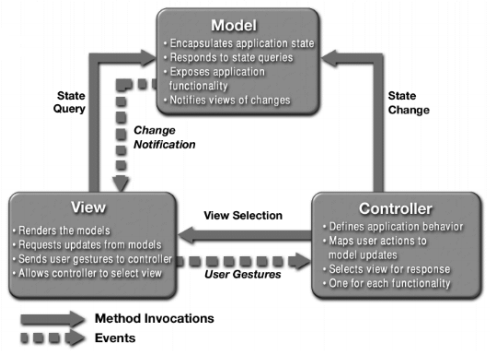
\includegraphics[scale=0.65]{Gambar/MVC}
	\caption{Diagram MVC}
	\end{figure}

Penjelasan MVC sebagai berikut \cite{Hans:2014}:

\begin{itemize}
	\item \textit{Model}\\
	Komponen ini berhubungan dengan proses yang ada dan juga terdapat di dalam sistem.\\
	Contoh model dalam skripsi ini adalah library Apache POI, iCal4j .
	\item \textit{Controller}\\
	Komponen yang mengatur komponen dari model ke view maupun sebaliknya. Fungsi dari komponen ini adalah sebagai penghubung komponen model dan view.\\
	Contoh \textit{Controller} di dalam skripsi ini adalah kode-kode dalam bahasa java yang meng-inherit dari kelas-kelas dalam \textit{library} Apache POI dan iCal4j untuk membaca \textit{file} excel dari TU dan mengkonversikannya dalam format iCalendar.
	\item \textit{View}\\
	komponen yang berhubungan dengan \textit{end user}. Bentuknya berupa tampilan yang akan digunakan oleh \textit{user} atau sering disebut sebagai \textit{user-interface}.
	Contoh \textit{view} dalam pengerjaan skripsi ini adalah kode-kode yang dituliskan dalam Java FX berupa \textit{file} yang berekstensi fxml.\\
	Banyak keuntungan dengan pendekatan MVC, yakni \cite{Hans:2014}:
	\begin{enumerate}
		\item Pembagian modul pengerjaan yang jelas untuk setiap orang di dalam suatu tim.
		\item Kemudahan untuk \textit{maintenance} dimasa depan.
		\item Mempunyai fleksibilitas tinggi dalam pengembangan,
	\end{enumerate}
\footnote{http://elmolya.blogspot.co.id/2010/03/belajar-mvc.html}
\end{itemize}

\section{Apache POI}

Apache POI pada hakikatnya merupakan API( \textit{application programming interface}) yang populer digunakan oleh programmer untuk membuat, memodifikasi, dan menampilkan \textit{file} MS Office menggunakan bahasa pemograman Java. Untuk mengingatkan bahwa API atau yang dalam bahasa indonesia disebut antarmuka pemograman aplikasi adalah sekumpulan perintah, fungsi, serta protokol yang digunakan oleh programmer saat membangun perangkat lunak \footnote{https://id.wikipedia.org/wiki/Antarmuka\_pemrograman\_aplikasi}. 

\begin{figure}[h]
	\centering
	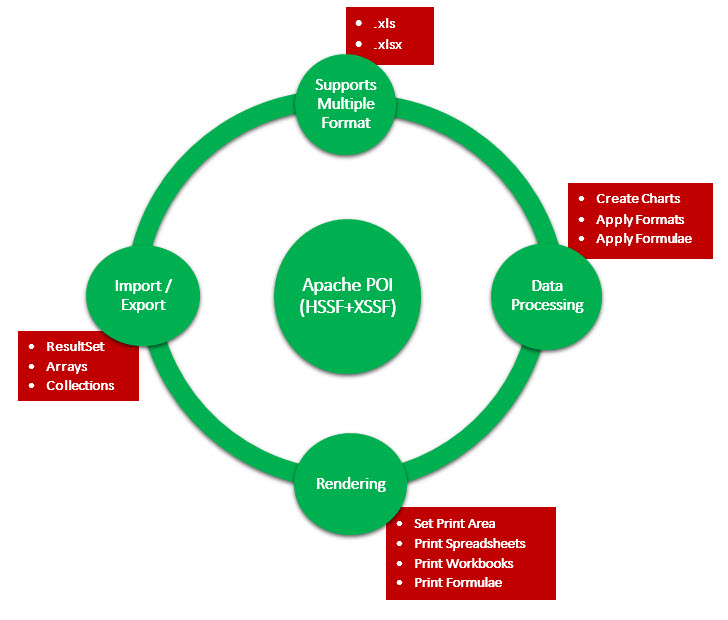
\includegraphics[scale=0.5]{Gambar/apachePOI}
	\caption{Kelebihan Apache POI(HSSF dan XSSF)} \cite{tutpoint}
	\end{figure}

\subsection{Komponen Apache POI}
Dalam Apache POI terdapat kelas dan method yang dapat bekerja dengan semua file OLE2 yang merupakan format file yang dipakai oleh dokumen dari Microsoft Office , seperti MS Word, Excel, dll \footnote{http://www.file-extensions.org/ole2-file-extension}. Berikut ini adalah komponen - komponen yang terdapat dalam Apache POI.\cite{tutpoint}

\begin{enumerate}
	\item \textbf{POIFS (\textit{Poor Obfuscation Implementation File System})} : Komponen ini merupakan faktor dasar dari semua elemen POI. Komponen ini dapat membaca file yang berbeda secara eksplisit.
	\item \textbf{HSSF (\textit{Horrible Spreadsheet Format})} : Komponen ini digunakan untuk membaca dan menulis format xls dari file MS-Excel.
	\item \textbf{XSSF (XML \textit{Spreadsheet Format})} : Komponen ini digunakan untuk membaca format file xlsx dari MS-Excel.
	\item \textbf{HPSF (\textit{Horrible Property Set Format})} : Komponen ini digunakan untuk mengekstrak perangkat file yang dimiliki oleh MS-Office.
	\item \textbf{HWPF (\textit{Horrible Word Proccessor Format})} : Komponen ini digunakan untuk menulis dan membaca ekstensi file doc dari MS-Word.
	\item \textbf{XWPF (\textit{XML Word Processor Format})} : Komponen ini digunakan untuk membaca dan menulis ekstensi file docx dari MS-Word.
	\item \textbf{HSLF (\textit{Horrible Slide Layout Format})} : Komponen ini digunakan untuk membaca, menulis, dan mengedit presentasi PowerPoint.
	\item \textbf{HDGF (\textit{Horrible Diagram Format})} : komponen ini berisi kelas dan method dari file binary MS-Visio.
	\item \textbf{HPBF (\textit{Horrible Publisher Format})} : Komponen ini digunakan untuk membaca dan menulis file MS-Publisher.
\end{enumerate}


\subsection{Kelas Inti Apache POI} 
Pada sub bab ini akan membahas sedikit intoduksi mengenai beberapa kelas dan method yang ada di Apache POI API yang merupakan bagian penting untuk bekerja dengan file excel mengunakan program Java.\cite{tutpoint}

\subsubsection{Workbook}
\textbf{org.apache.poi.ss.usermodel} \textit{package} merupakan \textit{super-interface} dari semua kelas yang berhubungan dengan pembuatan atau\textit{maintain} Excel workbook. Dua kelas yang mengimplementasikan \textit{interface} diatas sebagai berikut:\cite{tutpoint}
\begin{itemize}
	\item \textbf{HSSFWorkbook} : Kelas ini mempunyai method yang dapat membaca dan menulis file Microsoft Excel dengan format .xls. Kelas ini kompatibel dengan MS-Office versi 97-2003.
	\item \textbf{XSSFWorkbook} : Kelas ini mempunyai method untuk menulis dan membaca Microsoft Excel dan OpenOffice xml dengan format .xls atau .xlsx. Kelas ini kompatibel dengan MS-Office versi 2007 atau versi barunya.
\end{itemize}  


\subsubsection{HSSFWorkbook} 
HSSFWorkbook merupakan \textit{high-level class} dibawah \textbf{org.apache.xssf.usermodel} \textit{package}. HSSFWorkbook juga mengimplementasikan antarmuka workbook yang digunakan oleh file Excel dalam format .xls. Berikut ini list dari bebeberapa method dan constructor dalam kelas ini.\cite{tutpoint}\\

\noindent \textbf{Class Constructor}\\ \\


	\begin{tabular}{|c|p{12cm}|}
		\hline
		\textbf{No} & \textbf{Constructor dan Deskripsi} \\ \hline \hline
		1 & \textbf{HSSFWorkbook()}\\
			&	Membuat baru objek HSSFWorkbook.\\ \hline 
		2 & \textbf{HSSFWorkbook(DirectoryNode directory, boolean perserveNodes)}\\
			&	Membuat objek HSSFWorkbook baru dalam direktori yang spesifik.\\ \hline
		3 & \textbf{HSSFWorkbook(DirectoryNode directory, POIFSFileSystem fs, boolean perserveNodes)}\\
			&	Memberikan sebuah objek POIDSFileSystem dan sebuah spesifik didalamnya, serta membuat objek SSFWorkbook untuk membaca sebuah workbook yang spesifik.\\ \hline 
		4 & \textbf{HSSFWorkbook(java.io.InputStream s)}\\
			&	Membuat baru objek HSSFWorkbook menggunakan input stream.\\ \hline
		5 & \textbf{HSSFWorkbook(java.io.InputStream s, boolean preserveNodes )}\\
			&	Membangun sebuah POI \textit{file system} disekeliling input stream.\\ \hline
		6 & \textbf{HSSFWorkbook(POIFSFileSystem fs)}\\
			&	Membangun sebuah objek HSSFWorkbook baru menggunakan sebuah objek POIFSFileSystem.\\ \hline 		
		7 & \textbf{HSSFWorkbook(POIFSFileSystem fs, boolean preserveNodes)}\\
			&	Memberikan sebuah objek POIFSFileSystem dan membuat HSSFWorkbook baru untuk membacu sebuah workbook spesifik.\\ \hline 
	\end{tabular}

Berikut ini penjelasan parameter yang sering dipakai pada constructor :
\begin{itemize}
	\item \textbf{directory} : direktori proses dari POI filesystem
	\item \textbf{fs} : POI filesystem yang mengandung workbook stream.
	\item \textbf{preservenodes} : Opsional parameter yang memutuskan menjaga node lain, selain itu parameter ini menggunakan banyak memori seperti menyimpan semua POIFileSystem dalam memori(jika diset).
\end{itemize} 

\subsubsection{XSSFWorkbook}
Kelas ini merepresentasikan baik \textit{high} dan \textit{low} level format file excel. XSSFWorkbook merupakan kelas yang berada dalam \textit{package} \textbf{org.apache.xssf.usermodel} dan mengimplementasikan antarmuka workbook. Berikut ini list method dan constructor dalam kelas ini.\cite{tutpoint}
\\
\noindent \textbf{Class Constructor}\\ \\
	\begin{tabular}{|c|p{12cm}|}
		\hline
		\textbf{No} & \textbf{Constructor dan Deskripsi} \\ \hline \hline
		1 & \textbf{XSSFWorkbook()}\\
			&	Membuat baru objek XSSFWorkbook.\\ \hline 
		2 & \textbf{XSSFWorkbook(java.io.File file)}\\
			&	Membangun sebuah objek XSSFWorkbook dari file yang diberikan.\\ \hline
		3 & \textbf{XSSFWorkbook(java.io.InputStream is)}\\
			&	Membangun sebuah object XSSFWorkbook dengan \textit{buffering} semua input stream kedalam memory, dilanjutkan dengan membuka objek OPCPackage.\\ \hline 
		4 & \textbf{XSSFWorkbook(java.lang.String path)}\\
			&	Membangun sebuah objek XSSFWorkbook dengan diberikan \textit{full path} dari sebuah file.\\ \hline
	\end{tabular}
\\
\noindent \textbf{Class Methods}\\ \\

	\begin{tabular}{|c|p{12cm}|}
		\hline
		\textbf{No} & \textbf{Method dan Deskripsi} \\ \hline \hline
		1 & \textbf{CreateSheet()}\\
			&	Menciptakan sebuah XSSFSheet pada workbook, lalu menambahkan sheet, dan mengembalikannya dalam representasi \textit{high level} .\\ \hline 
		2 & \textbf{createSheet(java.lang.String sheetname)}\\
			&	Membuat sheet baru untuk workbook dan mengembalikannya dalam representasi \textit{high level}.\\ \hline
		3 & \textbf{createFont()}\\
			&	Membuat font baru dan menambahkannya pada tabel font workbook.\\ \hline 
		4 & \textbf{createCellStyle()}\\
			&	Membuat XSSFCellStyle Baru dan mmenambahkannya pada tabel style workbook.\\ \hline
		5 & \textbf{setPrintArea(int sheetIndex, int startColumn, int endColumn, int startRow,int endRow)}\\
			&	Menentukan area print dari kertas yang diberikan dengan parameter yang spesifik.\\ \hline	
	\end{tabular}
	
	
\subsubsection{Sheet}
Sheet merupakan sebuah interface dibawah package org.apache.ss.usermodel dan sheet merupakan super-interface dari semua kelas yang menciptakan \textit{high} atau \textit{low level spreadsheet} dengan nama yang spesifik. Jenis yang paling umum dari spreadsheet adalah worksheet yang direpresentasikan sebagai sebuah \textit{grid} dari cell.\cite{tutpoint}

\subsubsection{HSSFSheet}
HSSFSheet merupakan kelas dibawah \textit{package}\textbf{org.apache.poi.hssf.usermodel}. HSSFSheet dapat membuat excel spreadsheet dan memungkinkan untuk memformat style dari sheet dan data sheet.\cite{tutpoint}
\\
\noindent \textbf{Class Constructor}\\ \\
	\begin{tabular}{|c|p{12cm}|}
		\hline
		\textbf{No} & \textbf{Constructor dan Deskripsi} \\ \hline \hline
		1 & \textbf{HSSFSheet(HSSFWorkbook workbook)}\\
			&	Membuat baru HSSFSheet yang disebut HSSFWorkbook dalam pembuatan sheet baru .\\ \hline 
		2 & \textbf{HSSFSheet(HSSFWorkbook workbook, InternalSheet sheet)}\\
			&	Membuat sebuah HSSFSheet yang mewakili objek sheet yang diberikan.\\ \hline
	\end{tabular}
	
\subsubsection{XSSFSheet}
Kelas ini merupakan representasi dari \textit{high level} excel spreadsheet. Kelas ini berada dibawah package org.apache.poi.hssf.usermodel.\cite{tutpoint}
\\
\noindent \textbf{Class Constructor}\\ \\
	\begin{tabular}{|c|p{12cm}|}
		\hline
		\textbf{No} & \textbf{Constructor dan Deskripsi} \\ \hline \hline
		1 & \textbf{XSSFSheet()}\\
			&	Membuat baru XSSFSheet yang disebut XSSFWorkbook dalam pembuatan sheet baru .\\ \hline 
		2 & \textbf{XSSFSheet(PackagePart part, PackageRelationship rel)}\\
			&	Membuat sebuah XSSFSheet yang mewakili bagian package dan \textit{relationship}.\\ \hline
	\end{tabular}
\\
\noindent \textbf{Class Method}\\ \\
	\begin{tabular}{|c|p{12cm}|}
		\hline
		\textbf{No} & \textbf{Constructor dan Deskripsi} \\ \hline \hline
		1 & \textbf{addMergedRegion(CellRangeAddress region))}\\
			&	Menambahkan gabungan wilayah dari cell.(beberapa cell menjadi satu)   .\\ \hline 
		2 & \textbf{autoSizeColumn(int column)}\\
			& Menyesuaikan lebar kolom agar sesuai dengan isinya.\\ \hline
		3 & \textbf{iterator()}\\
			&	Method ini alias rowIterator() untuk memungkinkan foreach loop .\\ \hline
		4 & \textbf{addHyperlink(XSSFHyperlink hyperlink)}\\
			&	Mendaftarkan sebuah hyperlink kedalam koleksi hyperlink yang ada di sheet.\\ \hline	
	\end{tabular}

\subsubsection{Row}
Row merupakan interface berada dibawah \textit{package} \textbf{org.apache.poi.ss.usermodel}. Row ini digunakan untuk \textit{high-level representation} dari sebuah row pada sebuah spreadsheet. Row juga merupakan super-interface dari semua kelas yang mewakili row dalam POI \textit{Library}.\cite{tutpoint}

\subsubsection{XSSFRow}
XSSFRow merupakan sebuah kelas dibawah \textit{package} \textbf{org.apache.poi.xssf.usermodel} dan mengimplementasi Row interface. Selain itu, kelas ini dapat membuat row dalam sebuah spreadsheet. List dibawah ini merupakan method dan constructors pada kelas ini.\cite{tutpoint}
 \\ 
\noindent \textbf{Class Method}\\ \\
	\begin{tabular}{|c|p{12cm}|}
		\hline
		\textbf{No} & \textbf{Deskripsi} \\ \hline \hline
		1 & \textbf{createCell(int columnIndex)}\\
			&	Membuat cell baru dalam baris.\\ \hline 
		2 & \textbf{setHeight(short height)}\\
			&	Mengatur tinggi dalam satuan short.\\ \hline
	\end{tabular}

\subsubsection{Cell}
Cell merupakan interface yang berada dibawah \textit{package} \textbf{org.apache.poi.ss.usermodel}. Cell merupakan sebuah super-interface dari semua kelas yang mewakili cell dalam baris sebuah spreadsheet.\\

Cell dapat beruba berbagai atrubut seperti \textit{blank, numeric, date, error, } dll. Sebelum ditambahkan ke baris cell memiliki nomer tersendiri(dari mulai 0).\cite{tutpoint}

\subsubsection{XSSFCell}  
Kelas ini berada dibawah \textit{package} \textbf{org.apache.poi.xssf.usermodel}. Kelas ini mewakili cell interface. XSSFCell adalah \textit{high-level representation} cell dalam row dari sebuah spreadsheet.\cite{tutpoint}

\subsubsection{Ringkasan Tipe Cell}
List dibawah ini adalah sebagian \textit{field} dari kelas XSSFCell beserta deskripsinya.\\

	\begin{tabular}{|c|c|}
		\hline
		\textbf{Tipe Cell} & \textbf{Deskripsi} \\ \hline \hline
		CELL\_TYPE\_BLANK & Representasi cell kosong\\ \hline 
		CELL\_TYPE\_BOOLEAN &	Representasi cell Boolean (True atau False)\\ \hline 
		CELL\_TYPE\_ERROR & Representasi nilai error dari cell\\ \hline
		CELL\_TYPE\_FORMULA	&	Representasi dari hasil sebuah formula dalam cell\\ \hline
		CELL\_TYPE\_NUMERIC	&	Representasi dari data numerik dalam cell\\ \hline
		CELL\_TYPE\_STRING	&	Representasi dari String(teks) dalam cell\\ \hline
	\end{tabular}
	\\
	
\noindent \textbf{Class Method}\\ \\
	\begin{tabular}{|c|p{12cm}|}
		\hline
		\textbf{No} & \textbf{Deskripsi} \\ \hline \hline
		1 & \textbf{setCellStyle(CellStyle style)}\\
			&	Mengatur style untuk cell.\\ \hline 
		2 & \textbf{setCellType(int cellType)}\\
			&	Mengatur tipe cell (numeric, formula, atau String).\\ \hline
		3 & \textbf{setCellValue(boolean value)}\\
			&	Mengatur nilai bolean dalam sebuah cell.\\ \hline
		4 & \textbf{setCellValue(java.util.Calendar value)}\\
			&	Mengatur nilai tanggal dari cell .\\ \hline	
		5 & \textbf{setCellValue(double value)}\\
			&	Mengatur nilai numerik dari cell.\\ \hline
		6 & \textbf{setCellValue(java.lang.String str)}\\
			&	Mengatur nilai String dari cell.\\ \hline
		7 & \textbf{setHyperlink(Hyperlink hyperlink)}\\
			&	Menambahkan sebuah hyperlink kedalam cell\\ \hline					
	\end{tabular}

\subsubsection{XSSFCellStyle}
XSSFCellStyle merupakan sebuah kelas yang berada dibawah \textit{package} \textbf{org.apache.poi.usermodel}. kelas ini memberikan infomarsi yang mungkin mengenai format konten pada suatu cell dari spreadsheet. Kelas ini juga memberikan opsi untuk merubah format tersebut. Kelas ini mewakili CellStyle interface.\cite{tutpoint}

\subsubsection{Ringkasan Cell Style}
List dibawah ini adalah sebagian \textit{field} yang diwariskan dari CellStyle interface.\cite{tutpoint}\\

	\begin{tabular}{|c|c|}
		\hline
		\textbf{Nama Field} & \textbf{Deskripsi Field} \\ \hline \hline
		ALIGN\_CENTER & Rata tengah konten cell\\ \hline 
		ALIGN\_CENTER\_SELECTION &	Posisi seleksi tengah horizontal\\ \hline 
		ALIGN\_FILL & Mencocokan ukuran konten cell \\ \hline
		ALIGN\_JUSTIFY	&	Mencocokan ukuran konten cell terhadap lebarnya\\ \hline
		ALIGN\_LEFT	&	Rata kiri konten cell\\ \hline
		ALIGN\_RIGHT &	Rata kanan konten cell\\ \hline
		BORDER\_DASH\_DOT &	Cell style dengan garis dan titik \\ \hline
		BORDER\_DOTTED &	Cell style dengan border titik\\ \hline
		BORDER\_DASHED &	Cell Style dengan border garis\\ \hline
		BORDER\_THICK &	Cell Style dengan border tebal\\ \hline
		BORDER\_THIN &	Cell Style dengan border tipis\\ \hline
		VERTICAL\_BOTTOM &	Posisi konten cell vertikal kebawah\\ \hline
		VERTICAL\_CENTER &	Posisi konten cell vertikal ketengah\\ \hline
		VERTICAL\_JUSTIFY &	Posisi konten cell sejajar secara vertikal \\ \hline
		VERTICAL\_TOP &	Posisi selaras keatas secara vertikal\\ \hline
	\end{tabular}
\\
\noindent \textbf{Class Constructor}\\ \\
	\begin{tabular}{|c|p{15cm}|}
		\hline
		\textbf{No} & \textbf{Constructor dan Deskripsi} \\ \hline \hline
		1 & \textbf{XSSFCellStyle(int cellXfId, int cellStyleXfId, StylesTable stylesSource, ThemesTable theme)}\\
			&	Menciptakan cell style dengan bagian yang sudah disediakan.\\ \hline
		2 & \textbf{XSSFCellStyle(StylesTable stylesSource)}\\
			&	Membuat cell Style kosong.\\ \hline 	
	\end{tabular}
\\
\noindent \textbf{Class Method}\\ \\
	\begin{tabular}{|c|p{12cm}|}
		\hline
		\textbf{No} & \textbf{Method dan Deskripsi} \\ \hline \hline
		1 & \textbf{setAlignment(short align)}\\
			&	Mengatur style secara horizontal untuk cell.\\ \hline 
		2 & \textbf{setBorderBottom(short border)}\\ \hline
		3 & \textbf{setBorderColor(XSSFCellBorder.BorderSide side, XSSFColor color)}\\
			&	Mengatur warna untuk border yang dipilih.\\ \hline
		4 & \textbf{setBorderLeft(Short border)}\\
			&	Mengatur tipe border untuk border kiri dari cell .\\ \hline	
		5 & \textbf{setBorderRight(short border)}\\
			&	Mengatur tipe border untuk border kanan dari cell .\\ \hline
		6 & \textbf{setBorderTop(short border)}\\
			&	Mengatur tipe border untuk border atas dari cell \\ \hline
		7 & \textbf{setFillBackgroundColor(XSSFColor color)}\\
			&	Mengatur latar belakang warna yang diwakili oleh nilai XSSFColor\\ \hline
		8 & \textbf{setFillForegroundColor(XSSFColor color)}\\
			&	Mengatur latar depan warna yang diwakili oleh nilai XSSFColor\\ \hline
		9 & \textbf{setFillPattern(short fp)}\\
			&	Menentukan isi informasi cell dengan pola dan warna solid\\ \hline
	  10 & \textbf{setFont(Font font)}\\
			 &	Mengatur font\\ \hline
		11 & \textbf{setRotation(short rotation)}\\
			 &	Mengatur derajat rotasi pada teks dalam cell.\\ \hline
		12 & \textbf{setVerticalAlignment(short align)}\\
			 &	Menetapkan tipe posisi vertical pada cell\\ \hline		
	\end{tabular}

\subsubsection{HSSFColor}
HSSFColor merupakan sebuah kelas dibawah \textit{package} \textbf{org.apache.poi.hssf.util.package}. Kelas ini memberikan warna berbeda terhadap \textit{nested class}. Biasanya \textit{nested class} diwakili dengan menggunakan index masing-masing. Kelas ini mengimplementasikan Color interface.\cite{tutpoint}

	
\subsubsection{Nested Class}
Semua \textit{nested class} dari kelas ini adalah static dan setiap kelas memiliki index masing-masing. Warna kelas ini digunakan pada format cell seperti konten cell, border, latar depan(\textit{foreground}), dan latar belakang(\textit{background}). List dibawah ini merupakan sebagian dari \textit{nested class}.\cite{tutpoint}

\begin{tabular}{|c|c|}
		\hline
		\textbf{No} & \textbf{Nama Kelas(warna)} \\ \hline \hline
		1 & HSSFColor.AQUA\\ \hline 
		2 &	HSSFColor.AUTOMATIC\\ \hline 
		3 & HSSFColor.BLACK \\ \hline
		4	&	HSSFColor.BLUE\\ \hline
		5	&	HSSFColor.BRIGHT\_GREEN\\ \hline
		6 &	HSSFColor.BRIGHT\_GRAY\\ \hline
		7 &	HSSFColor.CORAL \\ \hline
		8 &	HSSFColor.DARK\_BLUE\\ \hline
		9 &	HSSFColor.DARK\_GREEN\\ \hline
		10 &	HSSFColor.SKY\_BLUE\\ \hline
		11 &	HSSFColor.WHITE\\ \hline
		12 &	HSSFColor.YELLOW\\ \hline
	\end{tabular}
	\\
	\noindent \textbf{Class Method}\\ \\
	Hanya satu method dalam kelas ini yang penting dan digunakan untuk mendapat nilai indeks.\\
	\begin{tabular}{|c|p{12cm}|}
		\hline
		\textbf{No} & \textbf{Method dan Deskripsi} \\ \hline \hline
		1 & \textbf{getIndex()}\\
			&	Method ini digunakan untuk mendapatkan nilai indeks dari sebuah \textit{nested class}.\\ \hline 
	\end{tabular}
	
\subsubsection{XSSFColor}
XSSFColor merupakan sebuah kelas dibawah \textit{package} \textbf{org.apache.poi.xssf.usermodel}. Kelas ini mewakili warnma pada spreadsheet. Kelas ini mengimplementasika interface warna. List dibawah ini merupakan beberapa method XSSFColor dan constructornya.\cite{tutpoint}
\\
\noindent \textbf{Class Constructor}\\ \\
	\begin{tabular}{|c|p{12cm}|}
		\hline
		\textbf{No} & \textbf{Constructor dan Deskripsi} \\ \hline \hline
		1 & \textbf{XSSFColor()}\\
			&	Menciptakan \textit{instance} baru dari XSSFColor.\\ \hline
		2 & \textbf{XSSFColor(byte[] rgb)}\\
			&	Membuat  \textit{instance} baru dari XSSFColor menggunakan RGB.\\ \hline
		3 & \textbf{XSSFColor(java.awt.Color clr))}\\
			&	Membuat  \textit{instance} baru dari XSSFColor menggunakan kelas warna dari \textit{awt package}.\\ \hline 		
	\end{tabular}
\\ \\
\noindent \textbf{Class Methods}\\ \\
	\begin{tabular}{|c|p{12cm}|}
		\hline
		\textbf{No} & \textbf{Method dan Deskripsi} \\ \hline \hline
		1 & \textbf{setAuto(boolean auto)}\\
			&	Mengatur sebuah nilai boolean untuk mengindikasikan bahwa ctColor bersifat otomatis dan bergantung pada ctColor sistem.\\ \hline
		2 & \textbf{setIndexed(int indexed)}\\
			&	Mengatur nilai indeks ctColor sebagai sistem ctColor.\\ \hline
	\end{tabular}

\subsubsection{XSSFFFont}
XSSFFont merupakan kelas dibawah \textit{package} \textbf{org.aoache.poi.xssf.usermodel}. Kelas ini mengimplementasikan \textit{Font interface} dan oleh sebab itu kelas ini dapat menangani font berbeda pada sebuah workbook.\cite{tutpoint}
\\
\noindent \textbf{Class Constructor}\\ \\
	\begin{tabular}{|c|p{12cm}|}
		\hline
		\textbf{No} & \textbf{Constructor dan Deskripsi} \\ \hline \hline
		1 & \textbf{XSSFFont()}\\
			&	Menciptakan \textit{instance} baru dari XSSFFont.\\ \hline
	\end{tabular}
\\ \\
\noindent \textbf{Class Methods}\\ \\
	\begin{tabular}{|c|p{12cm}|}
		\hline
		\textbf{No} & \textbf{Method dan Deskripsi} \\ \hline \hline
		1 & \textbf{setBold(boolean bold)}\\
			&	Mengatur sebuah nilai boolean untuk atribut 'bold'.\\ \hline
		2 & \textbf{setColor(short color)}\\
			&	Mengatur nilai indeks warna untuk font.\\ \hline
		3 & \textbf{setColor(XSSFColor color)}\\
			&	Mengatur warna untuk font dalam standar nilai warna Alpha RGB.\\ \hline
		4 & \textbf{setFontHeight(short height)}\\
			&	Mengatur tinggi font dalam poin.\\ \hline
		5 & \textbf{setFontName(java.lang.String name)}\\
			&	Mengatur nama dari font.\\ \hline
		6 & \textbf{setItalic(boolean italic)}\\
			&	Mengatur nilai boolean pada poperti 'italic'.\\ \hline					
	\end{tabular}
	
\subsubsection{XSSFHyperlink}
XSSFHyperlink merupakan kelas dibawah \textit{package} \textbf{org.apache.poi.xssf.usermodel}. Kelas ini mengimplementasikan \textit{Hyperlink interface}. Kelas ini digunakan untuk mengatur sebuah hyperlink pada konten cell dalam sebuah spreadsheet.\cite{tutpoint}
\\
\noindent \textbf{Field}\\
Field dalam kelas ini akan didefinisikan sebagai berikut. Field disini dalam arti tipe dari hyperlink yang dipakai.\\
\begin{tabular}{|c|c|}
		\hline
		\textbf{Field} & \textbf{Deskripsi} \\ \hline \hline
		LINK\_DOCUMENT & Dipakai untuk menghubungkan dengan dokumen lainnya\\ \hline 
		LINK\_EMAIL &	Digunakan untuk menghubungkan dengan email\\ \hline 
		LINK\_FILE & Digunakan untuk menghubungkan dengan file lain dalam berbagai format \\ \hline
		LINK\_URL	&	Digunakan untuk menghubungkan dengan URL \textit{website}\\ \hline
	\end{tabular}
	\\ \\
	\noindent \textbf{Class Methods}\\ \\
	\begin{tabular}{|c|p{12cm}|}
		\hline
		\textbf{No} & \textbf{Method dan Deskripsi} \\ \hline \hline
		1 & \textbf{setAddress(java.lang.String address)}\\
			&	Alamat Hyperlink.\\ \hline
	\end{tabular}

\subsubsection{XSSFCreationHelper}
XSSFCreationHelper merupakan kelas dibawah \textit{package} \textbf{org.apache.poi.xssf.usermodel}. Kelas ini mengimplementasikan \textit{CreationHelper interface}. Kelas ini digunakan sebagai bentuk kelas pendukung untuk \textit{formula evaluation} dan penyusun hyperlink.\cite{tutpoint}
\\
\noindent \textbf{Class Methods}\\ \\
	\begin{tabular}{|c|p{12cm}|}
		\hline
		\textbf{No} & \textbf{Method dan Deskripsi} \\ \hline \hline
		1 & \textbf{createFormulaEvaluator()}\\
			&	Membuat sebuh \textit{instance} XSSFFormulaEvaluator, objek yang dapat mengevaluasi formula dalam cell.\\ \hline
		2 & \textbf{createHyperlink(int type)}\\
			&	Membuat sebuah XSSFHyperlink baru.\\ \hline
	\end{tabular}

\subsubsection{XSSFPrintSetup}
XSSFPrintSetup merupakan kelas dibawah \textit{package} \textbf{org.apache.poi.xssf.usermodel}. Kelas ini mengimplementasikan \textit{PrintSetup interface}. Kelas ini digunakan untuk mengatur ukuran cetak pada halaman, wilayah cetak, opsi, dan pengaturan.\cite{tutpoint}
\\
\noindent \textbf{Class Methods}\\ \\
	\begin{tabular}{|c|p{12cm}|}
		\hline
		\textbf{No} & \textbf{Method dan Deskripsi} \\ \hline \hline
		1 & \textbf{setLandscape(boolean ls)}\\
			&	Mengatur sebuah nilai boolean yang dapat mengijinkan atau menolak \textit{landscape printing}.\\ \hline
		2 & \textbf{setLeftToRight(boolean ltor)}\\
			&	Mengatur perintah ke kiri, kanan, atas, atau bawah ketika proses cetak.\\ \hline
		3 & \textbf{setPaperSize(short size)}\\
			&	Mengatur ukuran kertas.\\ \hline
	\end{tabular}
	
\section{iCal4j}
iCal4j merupakan \textit{Java library} yang digunakan untuk membaca dan menulis data iCalendar yang didefinisikan dalam RFC2445. iCalendar standar menyediakan sebuah format data yang umumnya digunakan untuk menyimpan informasi tentang spesifikasi kalender seperti acara, pertemuan, \textit{to-do list}, dll. Semua \textit{tool} kalender yang populer, seperti Lotus Notes, Outlook, Google Calendar, Apple iCal mensupport standar iCalendar.\cite{ical}
\\ \\
Sebagai pengurai kalender dan \textit{object model}, iCal4j memudahkan untuk memodifikasi data kalender yang sudah ada atau membuat model data baru. Validasi juga diperlukan untuk memastikan data terjaga baik dan konsisten dengan spesifikasi yang diperlukan.\cite{ical}


\subsection{Komponen iCal4j}
Berikut ini merupakan kumpulan \textit{package} yang ada dalam iCal4j.\cite{ical}\\
\begin{tabular}{|c|p{12cm}|}
		\hline
		\textbf{No} & \textbf{Package dan Deskripsi} \\ \hline \hline
		1 & \textbf{net.fortuna.ical4j.data}\\
			&	Menyediakan berbagai tipe RFC2445 input, output, serta fungsi parsing.\\ \hline
		2 & \textbf{net.fortuna.ical4j.filter}\\
			&	Aturan untuk menyaring list komponen yang digunakan, \textit{properties}, maupun parameter yang digunakan.\\ \hline
		3 & \textbf{net.fortuna.ical4j.model}\\
			&	Berisikan komponen utama yang digunakan untuk mendefinisikan model iCalendar.\\ \hline
		4 & \textbf{net.fortuna.ical4j.model.component	
}\\
			&	Berisikan respresentasi tipe yang digunakan dalam komponen model iCalendar.\\ \hline
		5 & \textbf{net.fortuna.ical4j.model.parameter}\\
			&	Berisikan respresentasi tipe yang digunakan dalam parameter model iCalendar.\\ \hline
		6 & \textbf{net.fortuna.ical4j.model.property}\\
			&	Berisikan respresentasi tipe yang digunakan dalam properti model iCalendar.\\ \hline
		7 & \textbf{net.fortuna.ical4j.transform}\\
			&	Berisikan perubahan tipe yang digunakan komponen model iCalendar sesuai RFC2446   .\\ \hline
		8 & \textbf{net.fortuna.ical4j.util}\\
			&	Berisikan tipe utilitas yang mendukung fungsi dari iCal4j.\\ \hline							
	\end{tabular}

\subsection{Kelas Inti dari iCal4j}
Pada bagian ini \textit{package} yang ditulis di sub bab sebelumnya akan dijelaskan lebih dalam apa kegunaannya.\cite{ical}

\subsection{net.fortuna.ical4j.data}

\noindent \textbf{Ringkasan Interface}\\ \\
	\begin{tabular}{|c|p{12cm}|}
		\hline
		\textbf{No} & \textbf{Method dan Deskripsi} \\ \hline \hline
		1 & \textbf{CalendarParser}\\
			&	Pelaksana yang menyediakan fungsi parsing pada iCalendar.\\ \hline
		2 & \textbf{ContentHandler}\\
			&	Pelaksana yang menyediakan fungsi yang berlaku selama parsing aliran data dari iCalendar(misalnya membangun model objek).\\ \hline
	\end{tabular}
	\\ 
	\noindent \textbf{Ringkasan Kelas}\\ \\
	\begin{tabular}{|c|p{12cm}|}
		\hline
		\textbf{No} & \textbf{Method dan Deskripsi} \\ \hline \hline
		1 & \textbf{AbstractOutputter}\\
			&	kelas dasar untuk model \textit{output}.\\ \hline
		2 & \textbf{CalendarBuilder}\\
			&	Parsing dan memnagan sebuah model iCalendar dari input stream.\\ \hline
		3 & \textbf{CalendarOutputter}\\
			&	Menuliskan sebuah model iCalendar pada output stream.\\ \hline
		4 & \textbf{CalendarParserFactory}\\
			&	Menyediakan akses pada CalenderParser yang telah dikonfigurasi.\\ \hline
		5 & \textbf{CalendarParserImpl}\\
			&	Implementasi \textit{default} dari CalenderParser.\\ \hline
		6 & \textbf{DefaultCalendarParserFactory	
}\\
			&	Implementasi \textit{default} dari CalenderParser.\\ \hline
		7 & \textbf{FoldingWriter}\\
			&	Fungsi penulisan yang mendukung penulisan iCalendar berlipat.\\ \hline
		8 & \textbf{HCalendarParser}\\
			&	Menguraikan dokumen XHTML yang meliputi data kalender, ditandai dengan mikroformat hCalendar.\\ \hline
		9 & \textbf{HCalendarParserFactory}\\
			&	kumpulan parser untuk mikroformat hCal\\ \hline
		10 & \textbf{UnfoldingReader}\\
			&	Fungsi membaca bagian iCalendar yang wajib dibaca.\\ \hline
	\end{tabular}
	
\subsection{net.fortuna.ical4j.filter}

\noindent \textbf{Ringkasan Interface}\cite{ical}\\ \\
	\begin{tabular}{|c|p{12cm}|}
		\hline
		\textbf{No} & \textbf{Method dan Deskripsi} \\ \hline \hline
		1 & \textbf{Rule}\\
			&	Pelaksana yang menentukan apakah suatu objek tertentu diklasifikasikan sebagai pasangannya dapat dijadikan sebagai filter lampiran.\\ \hline
	\end{tabular}
	\\ \\
	\noindent \textbf{Ringkasan Kelas}\cite{ical}\\ \\
	\begin{tabular}{|c|p{12cm}|}
		\hline
		\textbf{No} & \textbf{Method dan Deskripsi} \\ \hline \hline
		1 & \textbf{DateInRangeRule}\\
			&	Mengimplementasikan Rule.\\ \hline
		2 & \textbf{Filter}\\
			&	Melakukan filtering dari seperangkat aturan. Sebuah filter dapat menentukan apakah setidaknya satu aturan tersebut cocok atau tidak. \\ \hline
		3 & \textbf{HasPropertyRule}\\
			&	Sebuah aturan yang mencocokan komponen memuat poperti yang spesifik.\\ \hline
		4 & \textbf{PeriodRule<T extends Component>	
}\\
			&	Sebuah aturan yang mencocokan komponen terjadi atau tidak dalam jangka waktu yang ditentukan.\\ \hline
	\end{tabular}
	
\subsection{net.fortuna.ical4j.model}

\noindent \textbf{Ringkasan Interface}\cite{ical}\\ \\
	\begin{tabular}{|c|p{12cm}|}
		\hline
		\textbf{No} & \textbf{Method dan Deskripsi} \\ \hline \hline
		2 & \textbf{Escapable}\\
			&	Pelaksana yang mengkonversi ke/dari nilai string kedalam bentuk iCalendar.\\ \hline
		4 & \textbf{ParameterFactory<T extends Parameter>}\\
			&	Pelaksana yang menyediakan pembuatan \textit{service} parameter.\\ \hline
		5 & \textbf{PropertyFactory<T extends Property>}\\
			&	Membuat properti iCalendar.\\ \hline
		6 & \textbf{TimeZoneRegistry}\\
			&	Menyediakan daftar definisi wilayah yang berlaku untuk digunakan objek iCalendar.\\ \hline
	\end{tabular}
	\\ \\
	\noindent \textbf{Ringkasan Kelas}\cite{ical}\\ \\
	\begin{tabular}{|c|p{12cm}|}
		\hline
		\textbf{No} & \textbf{Method dan Deskripsi} \\ \hline \hline
		1 & \textbf{AddressList}\\
			&	Mendefinisikan list dari alamat pada iCalendar.\\ \hline
		2 & \textbf{Calendar}\\
			&	Mendefinisikan kalendar pada iCalendar. \\ \hline
		3 & \textbf{CalendarDateFormatFactory}\\
			&	Membuat objek dateFormat untuk optimisasi pola tanggal pada iCalendar.\\ \hline
		4 & \textbf{Date}\\
			&	Representasi dari objek DATE sesuai RFC5445.\\ \hline
		5 & \textbf{DateList}\\
			&	Representasi list tanggal dari iCalendar.\\ \hline
		6 & \textbf{DateTime}\\
			&	Representasi dari objek DATE-TIME sesuai RFC5445.\\ \hline
		7 & \textbf{LocationTypeList}\\
			&	Menetapkan sebuah list tipe lokasi dari iCalendar.\\ \hline
		8 & \textbf{NumberList}\\
			&	Menetapkan list dari nomer.\\ \hline
		9 & \textbf{Parameter}\\
			&	Mendefinisikan parameter.\\ \hline
		10 & \textbf{Period}\\
			&	Mendefinisikan tenggat waktu.\\ \hline
		11 & \textbf{Property}\\
			&	Mendefinisikan properti dari iCalendar.\\ \hline		12 & \textbf{Time}\\
			&	Sebuah tipe yang merepresentasikan nilai waktu pada iCalendar.\\ \hline
		13 & \textbf{TimeZone}\\
			&	Implementasi zona waktu java.\\ \hline
		14 & \textbf{WeekDay}\\
			&	Mendefinisikan hari dalam seminggu dengan diimbangi terkait dengan kejadian bulanan atau tahunan.\\ \hline	
	\end{tabular}
	
\subsection{net.fortuna.ical4j.model.component}

	\noindent \textbf{Ringkasan Kelas}\cite{ical}\\ \\
	\begin{tabular}{|c|p{12cm}|}
		\hline
		\textbf{No} & \textbf{Method dan Deskripsi} \\ \hline \hline
		1 & \textbf{Available}\\
			&	Mendefinisikan komponen tersedia di iCalendar.\\ \hline
		2 & \textbf{Daylight}\\
			&	Mendefinisikan waktu siang dalam zona waktu. \\ \hline
		3 & \textbf{Standard}\\
			&	Mendefinisikan komponen zona waktu standar.\\ \hline
		4 & \textbf{Standard.Factory	 
VAlarm}\\
			&	Mendefinisikan komponen VALARM pada iCalendar.\\ \hline
		5 & \textbf{Standard.Factory	 
VAvailability}\\
			&	Mendefinisikan komponen VAvailability pada iCalendar.\\ \hline
		6 & \textbf{VAvailability.Factory	 
VEvent}\\
			&	Mendefinisikan komponen VEvent pada iCalendar.\\ \hline
		7 & \textbf{VEvent.Factory	 
VFreeBusy}\\
			&	Mendefinisikan komponen VFreeBusy pada iCalendar.\\ \hline
		8 & \textbf{VFreeBusy.Factory	 
VJournal}\\
			&	Mendefinisikan komponen VJournal pada iCalendar.\\ \hline
		9 & \textbf{VJournal.Factory	 
VTimeZone}\\
			&	Mendefinisikan komponen VTimeZone pada iCalendar.\\ \hline
		10 & \textbf{VTimeZone.Factory	 
VToDo}\\
			&	Mendefinisikan komponen VToDo pada iCalendar.\\ \hline
		11 & \textbf{VToDo.Factory	 
VVenue}\\
			&	Mendefinisikan komponen VVenue pada iCalendar.\\ \hline	
	\end{tabular}
	
\subsection{net.fortuna.ical4j.model.parameter}

	\noindent \textbf{Ringkasan Kelas}\cite{ical}\\ \\
	\begin{tabular}{|c|p{12cm}|}
		\hline
		\textbf{No} & \textbf{Method dan Deskripsi} \\ \hline \hline
		1 & \textbf{Abbrev}\\
			&	Mendefinisikan parameter singkatan.\\ \hline
		2 & \textbf{AltRep}\\
			&	Mendefinisikan alternatif representasi parameter teks. \\ \hline
		3 & \textbf{Cn}\\
			&	Mendefinisikan parameter dengan nama umum .\\ \hline
		4 & \textbf{CuType}\\
			&	Mendefinisikan tipe calender user.\\ \hline
		5 & \textbf{DelegatedFrom}\\
			&	Mendefinisikan parameter delegator.\\ \hline
		6 & \textbf{DelegatedTo}\\
			&	Mendefinisikan parameter delegasi.\\ \hline
		7 & \textbf{Dir}\\
			&	Mendefinisikan parameter referensi directory entri.\\ \hline
		8 & \textbf{Encoding}\\
			&	Mendefinisikan parameter inline Encoding.\\ \hline
		9 & \textbf{VJournal.Factory	 
VTimeZone}\\
			&	Mendefinisikan komponen VTimeZone pada iCalendar.\\ \hline
		10 & \textbf{FbType}\\
			&	Mendefinisikan tipe parameter \textit{free/busy}.\\ \hline
		11 & \textbf{FmtType}\\
			&	Mendefinisikan parameter tipe format.\\ \hline
		12 & \textbf{Language}\\
			&	Mendefinisikan parameter bahasa.\\ \hline
		13 & \textbf{Member}\\
			&	Mendefinisikan parameter list group peserta.\\ \hline
		14 & \textbf{PartStat}\\
			&	Mendefinisikan parameter satus partisipasi.\\ \hline
		15 & \textbf{Range}\\
			&	Mendefinisikan parameter identifikasi perulangan .\\ \hline
		16 & \textbf{Related}\\
			&	Mendefinisikan parameter pemicu alarm.\\ \hline
		17 & \textbf{RelType}\\
			&	Mendefinisikan parameter tipe hubungan.\\ \hline
		18 & \textbf{Rsvp}\\
			&	Mendefinisikan parameter RSVP.\\ \hline
		19 & \textbf{ScheduleAgent}\\
			&	Mendefinisikan penjadwalan.\\ \hline
		20 & \textbf{ScheduleStatus}\\
			&	Mendefinisikan status penjadwalan.\\ \hline
		21 & \textbf{SentBy}\\
			&	Mendefinisikan parameter pengirim.\\ \hline
		22 & \textbf{Type}\\
			&	Mendefinisikan parameter tipe.\\ \hline
		23 & \textbf{TzId}\\
			&	Mendefinisikan parameter zona waktu.\\ \hline
		24 & \textbf{Value}\\
			&	Mendefinisikan parameter nilai tipe data.\\ \hline
		25 & \textbf{Vvenue}\\
			&	Mendefinisikan parameter Vvenue.\\ \hline
		26 & \textbf{XParameter}\\
			&	Mendefinisikan parameter pemicu alarm.\\ \hline
		27 & \textbf{Related}\\
			&	Mendefinisikan penambahan parameter.\\ \hline
	\end{tabular}

\subsection{net.fortuna.ical4j.model.property}

	\noindent \textbf{Ringkasan Kelas}\cite{ical}\\ \\
	\begin{tabular}{|c|p{12cm}|}
		\hline
		\textbf{No} & \textbf{Method dan Deskripsi} \\ \hline \hline
		1 & \textbf{Action}\\
			&	Mendefinisikan aksi dari komponen properti iCalendar .\\ \hline
		2 & \textbf{Attach}\\
			&	Mendefinisikan lampiran dari komponen properti iCalendar. \\ \hline
		3 & \textbf{Attendee}\\
			&	Mendefinisikan kedatangan dari komponen properti iCalendar.\\ \hline
		4 & \textbf{BusyType}\\
			&	Mendefinisikan tipe sibuk pada komponen properti.\\ \hline
		5 & \textbf{Categories}\\
			&	Mendefinisikan kategori pada komponen properti.\\ \hline
		6 & \textbf{Clazz}\\
			&	Mendefinisikan kelas pada komponen properti.\\ \hline
		7 & \textbf{Comment}\\
			&	Mendefinisikan komen pada komponen properti.\\ \hline
		8 & \textbf{Completed}\\
			&	Mendefinisikan status selesai pada komponen properti.\\ \hline
		9 & \textbf{Contact}\\
			&	Mendefinisikan kontak pada komponen properti.\\ \hline
		10 & \textbf{Country}\\
			&	Mendefinisikan negara pada komponen properti.\\ \hline
		11 & \textbf{Created}\\
			&	Mendefinisikan pembuatan pada komponen properti.\\ \hline
		12 & \textbf{Description}\\
			&	Mendefinisikan deskripsi pada komponen properti.\\ \hline
		13 & \textbf{DtEnd}\\
			&	Mendefinisikan DtEnd pada komponen properti.\\ \hline
		14 & \textbf{DtStamp}\\
			&	Mendefinisikan DtStamp pada komponen properti.\\ \hline
		15 & \textbf{DtStart}\\
			&	Mendefinisikan DtStart pada komponen properti.\\ \hline
		16 & \textbf{Due}\\
			&	Mendefinisikan Due pada komponen properti.\\ \hline
		17 & \textbf{Duration}\\
			&	Mendefinisikan Durasi pada komponen properti.\\ \hline
		18 & \textbf{LastModified}\\
			&	Mendefinisikan terakhir dirubah pada komponen properti.\\ \hline
		19 & \textbf{Location}\\
			&	Mendefinisikan lokasi pada komponen properti.\\ \hline
		20 & \textbf{LocationType}\\
			&	Mendefinisikan tipe lokasi pada komponen properti.\\ \hline
		21 & \textbf{Name}\\
			&	Mendefinisikan nama pada komponen properti\\ \hline
		22 & \textbf{PercentComplete}\\
			&	Mendefinisikan progress pada komponen properti.\\ \hline
		23 & \textbf{Priority}\\
			&	Mendefinisikan prioritas pada komponen properti.\\ \hline
		24 & \textbf{RelatedTo}\\
			&	Mendefinisikan berhubungan dengan siapa pada komponen properti.\\ \hline
		25 & \textbf{Status}\\
			&	Mendefinisikan status pada komponen properti.\\ \hline
		26 & \textbf{StreetAddress}\\
			&	Mendefinisikan alamat pada komponen properti.\\ \hline
		27 & \textbf{Summary}\\
			&	Mendefinisikan ringkasan pada komponen properti.\\ \hline
		28 & \textbf{Url}\\
			&	Mendefinisikan url pada komponen properti.\\ \hline
		29 & \textbf{Version}\\
			&	Mendefinisikan versi pada komponen properti.\\ \hline	
	\end{tabular}

\subsection{net.fortuna.ical4j.model.transform}

	\noindent \textbf{Ringkasan Kelas}\cite{ical}\\ \\
	\begin{tabular}{|c|p{12cm}|}
		\hline
		\textbf{No} & \textbf{Method dan Deskripsi} \\ \hline \hline
		1 & \textbf{PublishTransformer}\\
			&	Merubah kalendar untuk dipublikasikan.\\ \hline
		2 & \textbf{Transformer}\\
			&	\textit{Base Class} untuk transforasi kalender. \\ \hline
		\end{tabular}
	
	\subsection{net.fortuna.ical4j.model.transform}

	\noindent \textbf{Ringkasan Kelas}\cite{ical}\\ \\
	\begin{tabular}{|c|p{12cm}|}
		\hline
		\textbf{No} & \textbf{Method dan Deskripsi} \\ \hline \hline
		1 & \textbf{PublishTransformer}\\
			&	Merubah kalendar untuk dipublikasikan.\\ \hline
		2 & \textbf{Transformer}\\
			&	\textit{Base Class} untuk transforasi kalender. \\ \hline
		\end{tabular}
		
	\subsection{net.fortuna.ical4j.model.util}

	\noindent \textbf{Ringkasan Interface}\cite{ical}\\ \\
	\begin{tabular}{|c|p{12cm}|}
		\hline
		\textbf{No} & \textbf{Method dan Deskripsi} \\ \hline \hline
		1 & \textbf{HostInfo}\\
			&	Menyediakan informasi host berupa\textit{paltform} yang independen.\\ \hline
	\end{tabular}
	
	\noindent \textbf{Ringkasan Kelas}\cite{ical}\\ \\
	\begin{tabular}{|c|p{12cm}|}
		\hline
		\textbf{No} & \textbf{Method dan Deskripsi} \\ \hline \hline
		1 & \textbf{Calendars}\\
			&	Method utility untuk bekerja dengan kalender.\\ \hline
		2 & \textbf{Dates}\\
			&	Mengimplementasikan koleksi dari method utility yang relevan untuk memproses tanggal. \\ \hline
		3 & \textbf{Numbers}\\
			&	kelas utility untuk memproses nomer. \\ \hline
		4 & \textbf{Strings}\\
			&	method utility yang bekerja dengan parameter. \\ \hline
		5 & \textbf{TimeZones}\\
			&	method utility yang relevan dengan zona waktu Java. \\ \hline
		\end{tabular}

\section{Java FX}
Java FX merupakan seperangkat grafis dan paket media yang memungkinkan pengembang untuk merancang, membuat, menguji, debug , dan dapat beroperasi secara konsisten di seluruh platform yang beragam.\\
Java FX dapat membuat berbagai macam aplikasi dari mulai aplikasi jaringan dasar hingga antar muka yang memiliki fitur audio, video, grafik, dan animasi



}{}
\ifdefstring{\vbabc}{1}{\chapter{Analisis}
\label{chap:analysis}
Pada bab ini, akan dijelaskan mengetai analisis kebutuhan dan fitur perangkat lunak, Diagram pengembangan perangkat lunak, \textit{use case} dari perangkat lunak serta diagram aktifitas dari perangkat lunak.
\section{Analisis Kebutuhan dan Fitur Perangkat Lunak}
\subsection{Analisis Kebutuhan}
Pertama-tama modul BI ini terintegrasi dengan ODOO, sebelum menggunakan modul ini maka pengguna diwajibkan untuk menginstall ODOO. Berikut ini \textit{requirement component} yang diperlukan untuk menginstall ODOO:
\begin{enumerate}
	\item \textit{installer} ODOO 8.0-20141128
	\item PosgreSQL 9.3
	\item Phyton 2.7
\end{enumerate} 
Sedangkan untuk minimum \textit{requirement hardware}, yaitu: 
\begin{enumerate}
	\item Intel x86 atau x64
	\item Minimum RAM 512 MB
	\item Minimum ruang di hardisk 150 MB
	\item Mendukung protokol TCP/IP
	\item OS x86 atau x64 MAC, Linux, atau Windows
\end{enumerate}
 
\subsection{Fitur Perangkat Lunak}
Perangkat Lunak ini akan memiliki fitur seperti gambar \textbf{3.1} :
\begin{figure}[h]
	\centering
	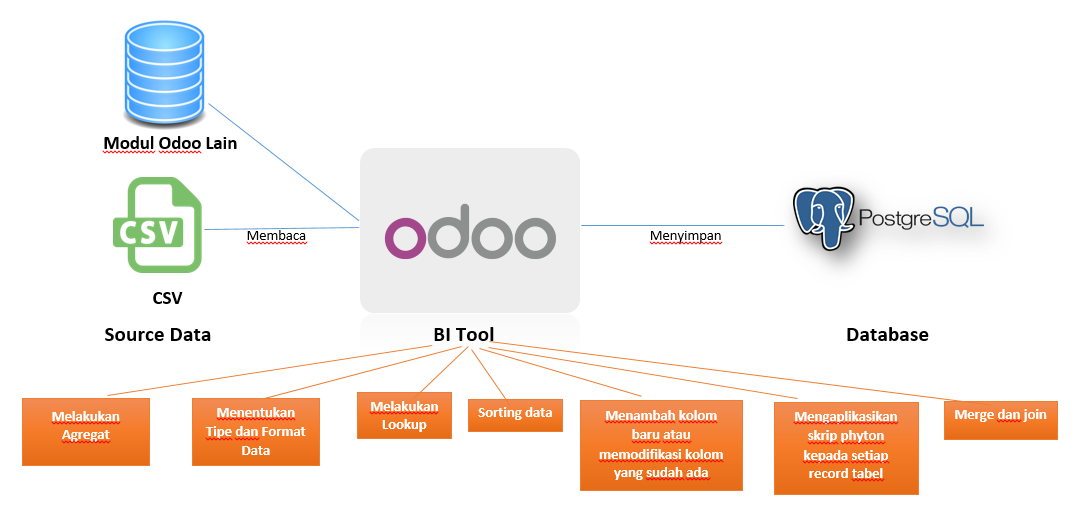
\includegraphics[scale=0.5]{Gambar/fitur-bi-tool}
	\caption{Fitur BI \textit{tool}}
	\end{figure}
	
	\begin{enumerate}
		\item BI \textit{tool} menerima dan membaca \textit{input source} berupa CSV/\textit{text file}, dan modul ODOO lain.
		\item Dapat menentukan tipe dan format data
		\item Dapat melakukan \textit{Lookup}
		\item Dapat melakukan agregat
		\item Dapat melakukan \textit{sorting} data
		\item Dapat menambah kolom baru atau memodifikasi kolom yang sudah ada
		\item Dapat mengaplikasikan skrip phyton terhadap setiap baris \textit{record}
		\item Dapat melakukan \textit{merge} dan \textit{join}
		\item Data yang telah diproses dapat disimpan dalam \texttt{database}
	\end{enumerate}
	
\subsection{Diagram Aktifitas pada BI \textit{Tool}}
	Pada subbab ini akan dibahas mengenai prosedur setiap aktifitas dari fitur yang diberikan oleh BI \textit{tool}.
	
	\subsubsection{Membuat Bisnis Baru}
	Sebelum melangkah pada proses ETL pengguna diwajibkan membuat nama bisnis untuk membedakan setiap proses ETL.
	Berikut ini step-step untuk membuat bisnis baru.
	\begin{figure}[h]
	\centering
	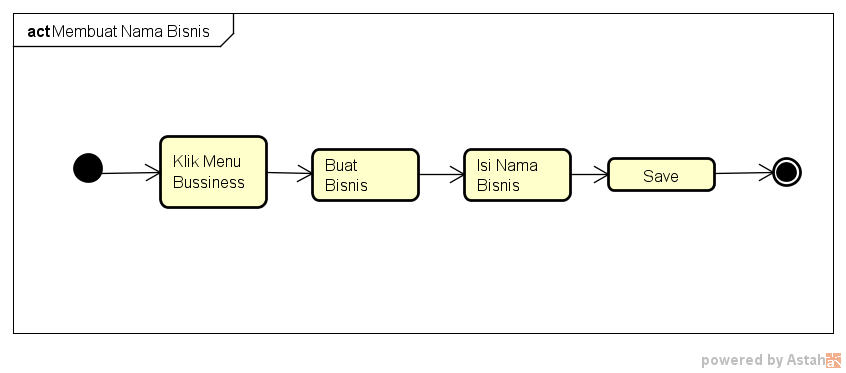
\includegraphics[scale=0.7]{Gambar/Membuat-Nama-Bisnis}
	\caption{Prosedur Membuat Bisnis Baru}
	\end{figure}
	
	\begin{enumerate}
		\item Pengguna mengklik menu \textit{Businesses}.
		\item Pengguna membuat nama bisnis baru.
		\item Pengguna mengisi kolom nama bisnis.
		\item Setelah selesai lalu pengguna mengklik tombol save.
	\end{enumerate}
	
	
	\subsubsection{Memasukan \textit{Data Source}}

	\begin{figure}[h]
	\centering
	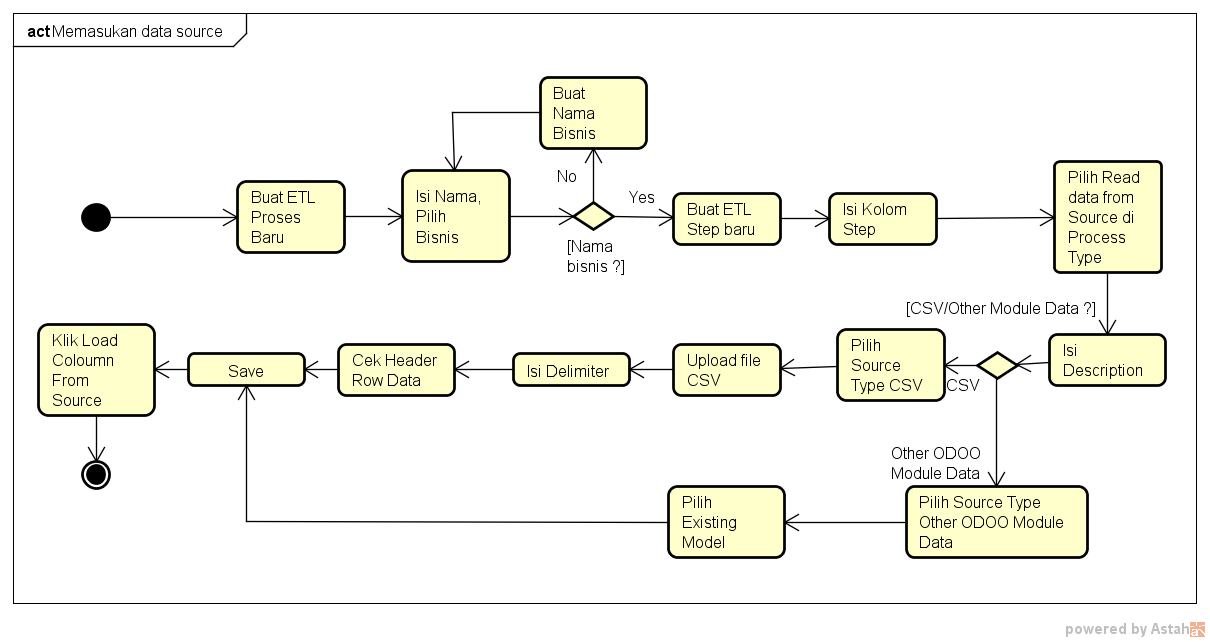
\includegraphics[scale=0.5]{Gambar/Memasukan-data-source}
	\caption{Prosedur Memasukan \textit{Data Source}}
	\end{figure}
	
	Pengguna dapat memasukan \textit{data source} bertipe CSV/\textit{teks file} atau modul ODOO lain dan menggunakannya sebagai sumber data untuk
	tipe proses lain dari fitur BI. Berikut tahapan-tahapan bagaimana memasukan data kedalam BI \textit{tool}.
	\begin{enumerate}
		\item Pengguna mengakses menu ETL \textit{Process} dan membuat proses ETL baru dengan menuliskan nama pada kolom nama yang tersedia.
		\item Selanjutnya pengguna memilih tipe bisnis yang telah dibuat sebelumnya, bila pengguna belum membuatnya maka pengguna dapat membuat nama bisnis terlebih dahulu sebelum melangkah ke proses selanjutnya.
		\item setelah kolom bisnis terisi maka pengguna membuat baru step etl 
		\item sesudahnya pengguna menuliskan nomer step untuk menentukan urutan \textit{compile} oleh BI \textit{tool}
		\item Pengguna memilih pilihan \textit{read data from source} dikolom \textit{process type} dilanjutkan dengan menuliskan deskripsi prosesnya pada kolom \textit{description}
		\item Pengguna dapat memilih tipe \textit{input} CSV atau Modul ODOO lain.
		\item Jika pengguna memilih tipe data CSV maka pada kolom \textit{source type} pilih CSV.
		\item Selanjutnya, Pengguna meng-\textit{upload} data CSV pada tempat yang disediakan
		\item Pengguna lalu mengisi kolom \textit{delimiter} dilanjutkan dengan menceklis kolom \textit{header row present?} bila baris pertama sumber data CSV adalah judul kolom.
		\item Jika pengguna memilih modul ODOO lain maka pada kolom \textit{source type} pilih \textit{other ODOO module data}.
		\item Setelah itu, pengguna memilih modul yang telah terinstal dalam odoo yang akan dijadikan \textit{source}.
		\item Setelah proses memilih \textit{source} selesai, Pengguna mengklik tombol \textit{save}, lalu mengklik kembali tombol \textit{load columns from source} untuk mengambil semua alamat kolom dalam \textit{source} untuk digunakan pada tipe proses selanjutnya.
	\end{enumerate}
	
\subsubsection{Menentukan Tipe dan Format Data}

	\begin{figure}[h]
	\centering
	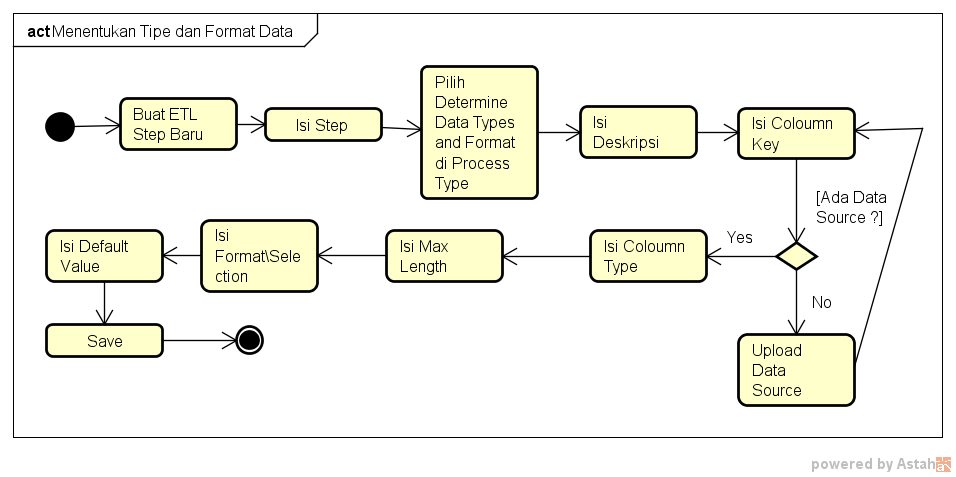
\includegraphics[scale=0.5]{Gambar/Menentukan-Tipe-dan-Format-Data}
	\caption{Prosedur Menentukan Tipe dan Format Data}
	\end{figure}

	Pengguna dapat menentukan tipe dan format data sesuai keinginan, namun syaratnya adalah \textit{data source} sudah di upload kedalam BI \textit{tool}. Berikut ini prosedur menentukan tipe data serta memformat data.
	\begin{enumerate}
		\item Membuat step ETL baru pada menu \textit{ETL process}.
		\item kemudian menuliskan nomer step pada kolom step, karena step pertama di isi oleh \textit{input data source} maka kolom step diisi oleh nomer yang lebih besar dari satu.
		\item Memilih \textit{determine data types and format} di kolom \textit{Process type}, dilanjutkan dengan mengisi kolom deskripsi.
		\item Selanjutnya mengisi \textit{Column key} 
		\item Dilanjutkan dengan mengisi \textit{column type}
		\item lalu menuliskan \textit{max length} untuk membatasi isi dari \textit{field} tersebut.
		\item Pengguna menuliskan \textit{format/selection} dari agar format data seragam dan terstandarisasi.
		\item Pengguna juga dapat mengisi kolom \textit{default value} bila diperlukan.
		\item Setelah proses selesai lalu pengguna mengklik tombol save dan semua setinggan yang telah dimasukan pengguna akan tersimpan dalam \textit{database}.
	\end{enumerate}
	
\subsubsection{Melakukan \textit{Lookup}}

	\begin{figure}[H]
	\centering
	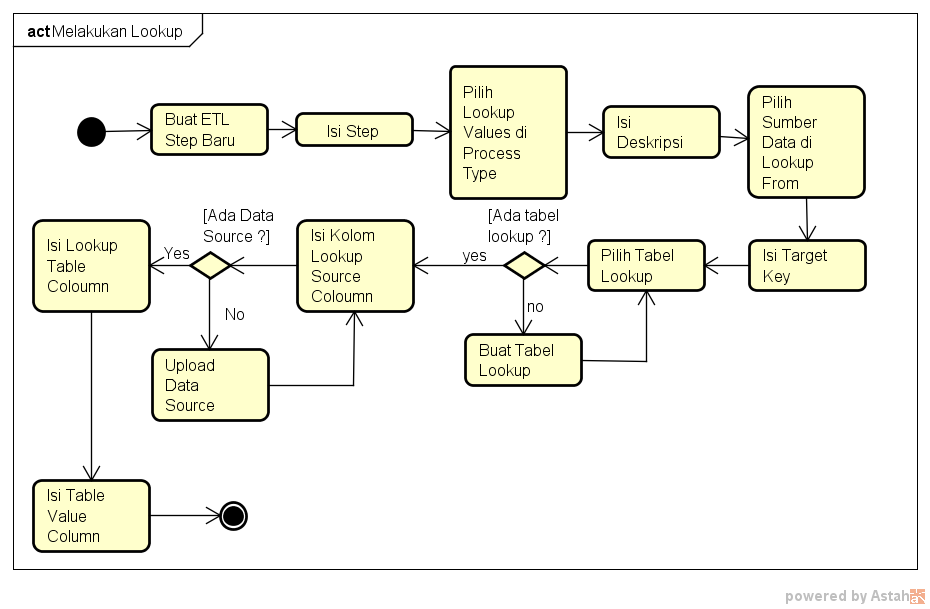
\includegraphics[scale=0.5]{Gambar/Melakukan-Lookup}
	\caption{Prosedur Melakukan \textit{Lookup}}
	\end{figure}

	Pengguna dapat melakukan \textit{lookup} dengan syarat \textit{data source} telah dimasukan kedalam \textit{database} BI tool. Berikut pemaparan proses penggunaan \textit{lookup}.
	\begin{enumerate}
		\item Pengguna membuat ETL step baru dengan mengisi nomer urutan dikolom step.
		\item Pengguna memilih \textit{process type} \textit{lookup values} serta menulis deskripsi step tersebut.
		\item Pengguna dapat memilih melakukan proses \textit{lookup} dengan tabel yang sudah ada didalam basis data BI tool atau menuliskan tabel baru pada kolom \textit{lookup value} dan \textit{result value}.
		\item pengguna menuliskan target \textit{field} yang akan disi.
		\item kemudian memilih \textit{value} kolom mana yang dijadikan acuan.
		\item setelah selesai pengguna mengklik tombol save untuk menyimpan setingan yang telah dimasukan sebelumnya.
	\end{enumerate}

\subsubsection{Melakukan \textit{Sorting Data}}
	\begin{figure}[H]
	\centering
	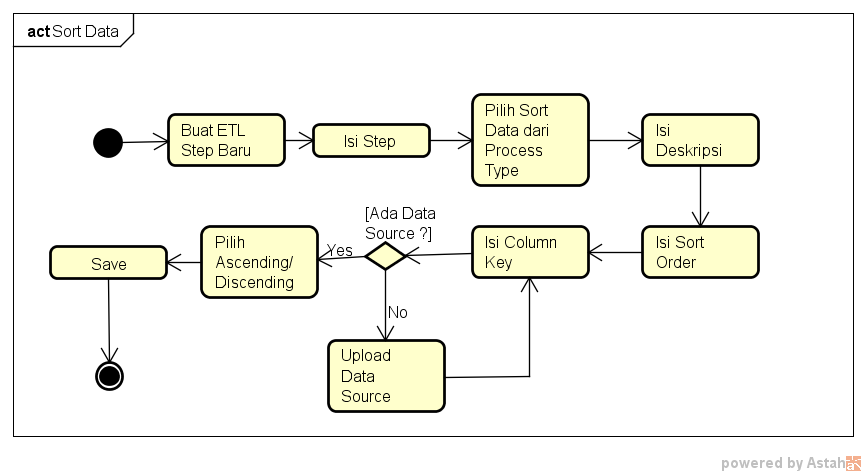
\includegraphics[scale=0.5]{Gambar/Sort-Data}
	\caption{Prosedur Melakukan \textit{Sorting Data}}
	\end{figure}
	
	Pada bagian ini pengguna dapat melakukan \textit{sorting data} dengan meng-\textit{input} sumber data terlebih dahulu. 
	Berikut penjelasan proses \textit{sort order}
	\begin{enumerate}
		\item Pengguna membuat ETL step baru dengan mengisi nomer urutan dikolom step.
		\item Selanjutnya memilih \textit{process type sort data} dilanjutkan dengan mengisi deskripsi proses tersebut.
		\item Pengguna menuliskan \textit{sort order} sesuai dengan urutan \textit{sort} yang terlebih dahulu di inginkan.
		\item Pengguna menuliskan \textit{column key} menandakan kolom \textit{source} mana yang akan diurutkan.
		\item Terakhir pengguna memilih \textit{direction} dari \textit{sort} yang di inginkan apakah \textit{ascending} atau \textit{descending}, lalu klik tombol \textit{save} untuk menyimpan semua \textit{setting} yang telah dilakukan.
	\end{enumerate}
	
\subsubsection{Menambah atau Memodifikasi Kolom}
	\begin{figure}[H]
	\centering
	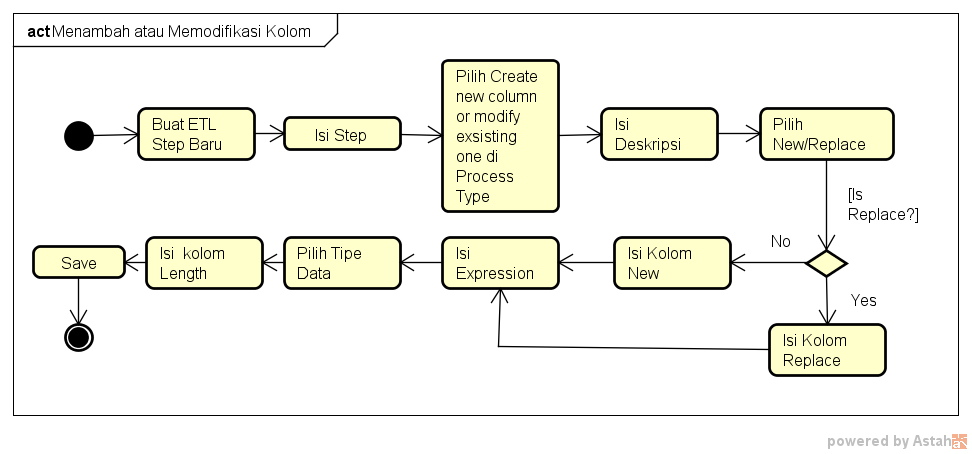
\includegraphics[scale=0.5]{Gambar/Menambah-atau-Memodifikasi-Kolom}
	\caption{Prosedur Menambah atau Memodifikasi Kolom}
	\end{figure}

	Pengguna dapat menambahkan kolom atau memodifikasi kolom yang tersedia dengan proses sebagai berikut.
	\begin{enumerate}
		\item Pengguna terlebih dahulu membuat ETL proses baru dan mengisi kolom step,
		\item Selanjutnya memilih \textit{create new column or modify existing one} pada kolom \textit{process type} dan menuliskan deskripsi dari proses tersebut.
		\item Pengguna menentukan apakan ingin menambahkan kolom baru atau memodifikasi kolom yang tersedia.
		\item Jika memodifikasi kolom tentukan kolom yang akan dimodifikasi.
		\item Jika membuat kolom baru pengguna menuliskan nama kolom baru.
		\item Setelah itu pengguna dapat menuliskan fungsi pyton untuk perhitungan atau tujuan lain pada kolom \textit{expression}.
		\item Pengguna menentukan tipe data kolom tersebut.
		\item Pengguna dapat menentukan panjang data yang akan dimasukan pada kolom \textit{length}.
		
	\end{enumerate}
	
\subsubsection{Mengaplikasikan Phyton \textit{Script}}

	\begin{figure}[H]
	\centering
	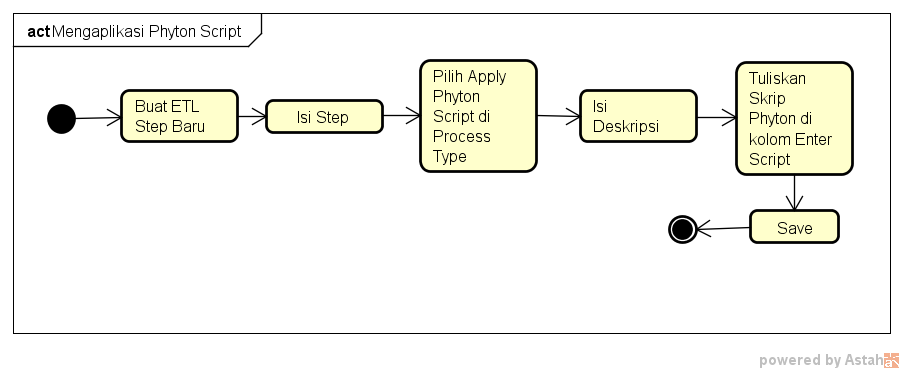
\includegraphics[scale=0.5]{Gambar/Mengaplikasikan-Phyton-Script}
	\caption{Prosedur Mengaplikasikan Phyton \textit{Script}}

	\end{figure}
	Pengguna dapat menjalankan skrip phyton yang berlaku untuk setiap baris data yang pada \textit{source}.
	Berikut proses memasukan skrip phyton pada BI \textit{tool}.
	\begin{enumerate}
		\item Pengguna membuat ETL step baru dengan mengisi nomer urutan dikolom step.
		\item Selanjutnya memilih \textit{process type apply phyton script to each data line} dilanjutkan dengan mengisi deskripsi proses tersebut.
		\item Setelah itu pengguna dapat langsung memasukan skrip phyton pada kolom \textit{enter script} pada perangkat lunak.
		\item Setelah selesai pengguna mengklik tombol save untuk menyimpan semua \textit{setting}.
	\end{enumerate}
	
\subsubsection{Melakukan Agregat}

	\begin{figure}[H]
	\centering
	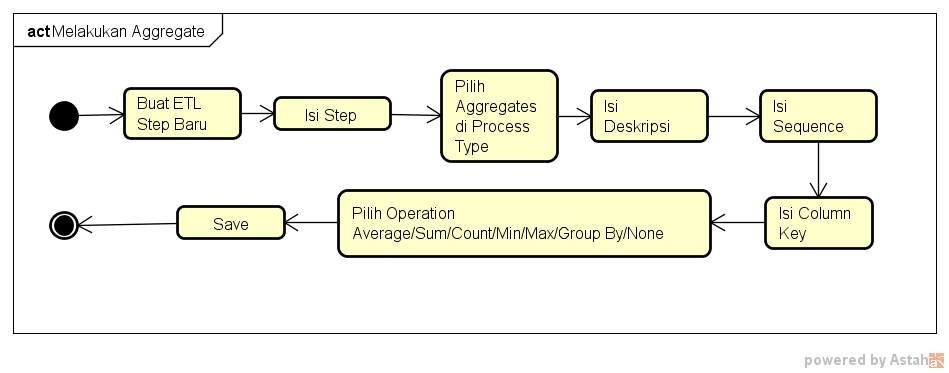
\includegraphics[scale=0.5]{Gambar/Melakukan-Aggregate}
	\caption{Prosedur Melakukan \textit{Aggregate}}
	\end{figure}	
	
	Pengguna dapat melakukan agregat terhadap \textit{data source}. Berikut pemaparan proses agregat.
	\begin{enumerate}
		\item Pengguna membuat ETL step baru dengan mengisi nomer urutan dikolom step.
		\item Pengguna memilih \textit{aggregates} pada kolom \textit{process type} dan menuliskan deskripsi mengenai proses tersebut.
		\item Pengguna menuliskan urutan dari pengerjaan agregat pada kolom \textit{sequence}.
		\item Pengguna memilih kolom yang akan di agregat.
		\item Pengguna memilih operasi yang dilakukan apakah \textit{count, max, min, sum, average, group by} ataupun \textit{none}.
		\item Setelah selesai pengguna mengklik tombol \textit{save}.
	\end{enumerate}
	
\subsubsection{Melakukan \textit{Merge Join}}

	\begin{figure}[H]
	\centering
	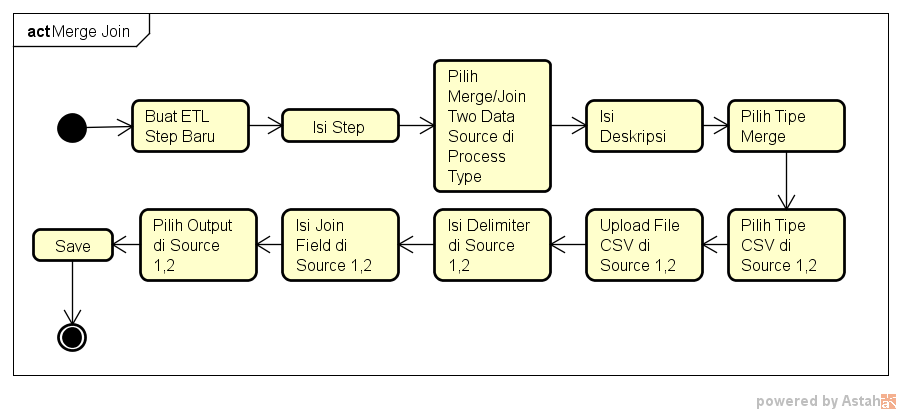
\includegraphics[scale=0.5]{Gambar/Merge-Join}
	\caption{Prosedur Melakukan \textit{Merge Join} dari dua \textit{data source}}
	\end{figure}

	Pengguna dapat melakukan \textit{merging} terhadap dua \textit{data source} sekaligus. Berikut pemaparan prosesnya. 
	\begin{enumerate}
		\item Pengguna membuat ETL step baru dengan mengisi nomer urutan dikolom step.
		\item Setelah itu memilih \textit{merge/join two data source} pada kolom \textit{process type} dan menuliskan deskripsi proses tersebut pada kolom \textit{description}.
		\item Pengguna memilih tipe \textit{merge} yang akan digunakan, yaitu \textit{left outer join}, \textit{inner join}, atau \textit{right outer join}.
		\item Pengguna menentukan tipe \textit{source}.
		\item Pengguna \textit{upload data source} jika tipe masukannya CSV.
		\item Pengguna mengisi kolom \textit{delimiter} jika tipe masukannya CSV.
		\item Setelah \textit{upload} selesai maka kolom pada \textit{source} akan terbaca otomatis oleh BI \textit{tool}.
		\item Setelah \textit{source} pertama selesai, pengguna melakukan step yang sama terhadap \textit{source} ke=2.
		\item Setelah kedua \textit{source} sudah terbacaa oleh BI tool, selanjutnya pengguna menuliskan \textit{join field} pada kedua kolom \textit{source} tersebut.
		\item Pengguna dapat menentukan \textit{output} kolom dengan menceklis mana saja yang akan menjadi \textit{output} dalam tabel destinasi pada bagian \textit{output} dalam BI \textit{tool}.
		\item Setelah semua selesai maka pengguna mengklik tombol \textit{save}.
	\end{enumerate}
	
	\subsubsection{\textit{Save to Database}}
	
	\begin{figure}[H]
	\centering
	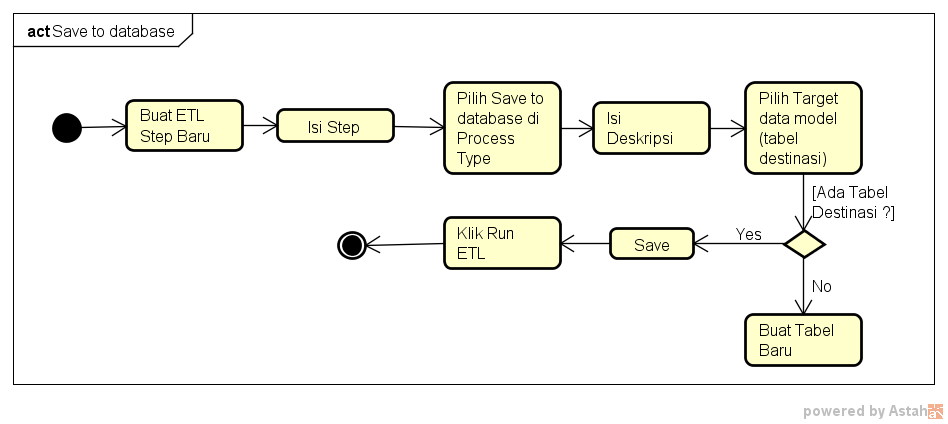
\includegraphics[scale=0.5]{Gambar/Save-to-database}
	\caption{Prosedur Menyimpan Data dalam \textit{Database}}
	\end{figure}
	
	Setelah semua tipe proses dilalui maka pengguna perlu menyimpan data hasil proses kedalam \textit{database} BI \textit{tool}. Namun, pastikan semua \textit{process type} telah terisi dengan benar, bila tidak hasil proses ETL tidak akan tersimpan dalam \textit{database}.  Untuk menyimpan data hasil proses kedalam tabel destinasi dalam \textit{database} syaratnya perlu minimal satu tipe proses \textit{read data from source} atau \textit{merge join} yang meminta \textit{input data source} pada pengguna. Berikut pemaparan lebih lanjut mengenai prosesnya.
\begin{enumerate}
	\item Pengguna membuat ETL step baru dengan mengisi nomer urutan dikolom step.
	\item Selanjutnya pengguna memilih \textit{save to database} pada kolom \textit{process type} dan menuliskan deskripsi singkat mengenai proses tersebut.
	\item Pengguna menentukan tabel destinasi tempat penyimpanan, dalam istilah ODOO disebut \textit{target data model}.
	\item Kolom destinasi akan terbaca secara otomatis oleh BI \textit{tool} setelah menentukan tabel destinasi/\textit{target data model}.
	\item Pengguna melakukan \textit{mapping} kolom dari \textit{source} mana yang akan masuk dalam tabel destinasi.
	\item Setelah semua selesai klik \textit{save}.
	\item Lalu, pengguna mengklik tombol \textit{Run ETL} untuk menjalankan semua tipe proses ETL dan menyimpannya dalam \textit{database}
\end{enumerate}
	
\section{Permodelan Tool}

Berikut diagram use case berserta skenario yang tertera pada gambar \textbf{3.10}

\begin{figure}[h]
	\centering
	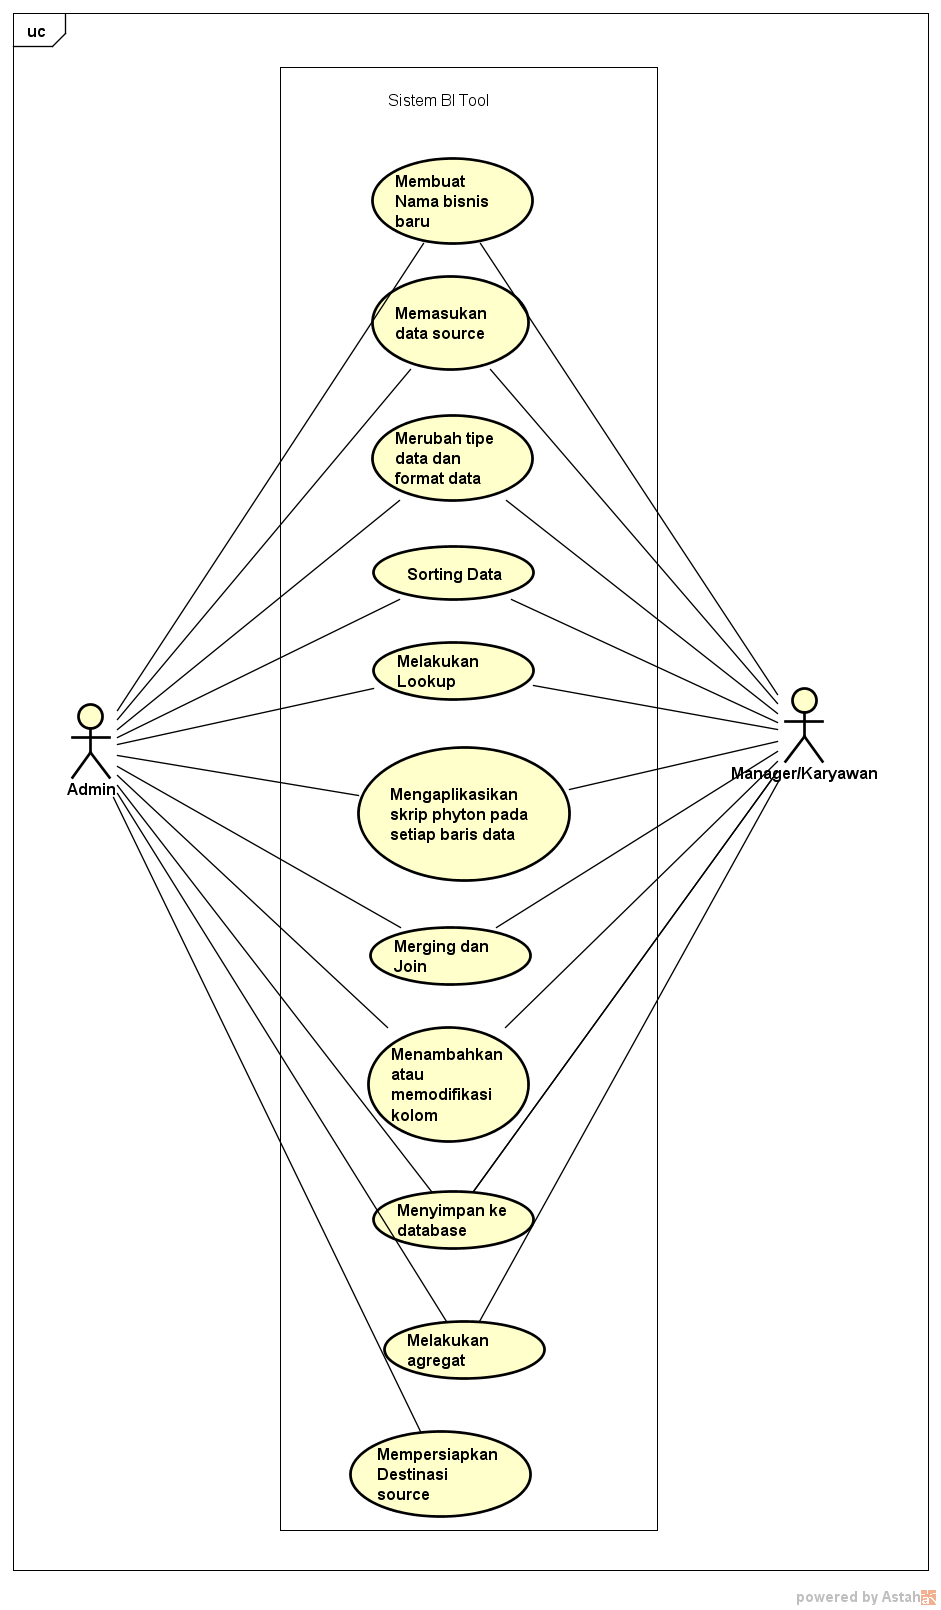
\includegraphics[scale=0.4]{Gambar/usecase-bi}
	\caption{Diagram use case BI \textit{tool}}
	\end{figure}

\begin{enumerate}
	\item Skenario Membuat Bisnis Baru \\
	{\renewcommand\labelitemi{}
		\begin{itemize}
			\item Deskripsi		: Kegiatan membuat nama bisnis.
			\item Aktor				: Admin, manajer
			\item Prakondisi	: -
			\item Skenario		:
				\begin{itemize}
					\item Admin, manajer dapat membuat nama bisnis baru 
				\end{itemize}
		\end{itemize}
		}
		
	\item Skenario Memasukan \textit{Data Source}
	{\renewcommand\labelitemi{}
	\begin{itemize}
			\item Deskripsi		: Kegiatan meng-\textit{upload} \textit{data source} berupa \textit{file} CSV atau teks.
			\item Aktor				: Admin, Manajer
			\item Prakondisi	: -
			\item Skenario		:
				\begin{itemize}
					\item Admin, manajer meng-\textit{upload} CSV atau file teks melalui menu ETL \textit{process}. 
				\end{itemize}
		\end{itemize}
		}
		
		\item Skenario Merubah Tipe dan Format Data
		{\renewcommand\labelitemi{}
		\begin{itemize}
			\item Deskripsi		: Kegiatan merubah tipe data dan format data.
			\item Aktor				: Admin, Manajer 
			\item Prakondisi	: \textit{data source} telah di\textit{input} sebelumnya.
			\item Skenario		:
				\begin{itemize}
					\item Admin, manajer dapat menentukan tipe data, format data, \textit{dafault value} maupun panjang data agar seragam.
				\end{itemize}
		\end{itemize}
		}
		
		\item Skenario \textit{Sorting Data}
		{\renewcommand\labelitemi{}
		\begin{itemize}
			\item Deskripsi		: Kegiatan mengurutkan data terhadap \textit{data source}.
			\item Aktor				: Admin, Manajer 
			\item Prakondisi	: \textit{data source} telah di\textit{input} sebelumnya
			\item Skenario		:
				\begin{itemize}
					\item Admin, manajer dapat mengurutkan data sesuai \textit{order penulisannya} dan dapat menentukan arah pengurutan secara menaik atau menurun.
				\end{itemize}
		\end{itemize}
		}
		
			\item Skenario Melakukan \textit{Lookup}
		{\renewcommand\labelitemi{}
		\begin{itemize}
			\item Deskripsi		: Kegiatan melakukan \textit{lookup} terhadap data \textit{input source}.
			\item Aktor				: Admin, Manajer 
			\item Prakondisi	: \textit{data source} dan data tabel yang akan di\textit{lookup} telah di\textit{input} sebelumnya jika ingin memilih \textit{lookup} dari \textit{existing table}
			\item Skenario		:
				\begin{itemize}
					\item Admin, manajer dapat melakukan \textit{lookup} terhadap \textit{data source} dengan data tabel yang telah ada dalam \textit{database} maupun data tabel yang dimasukan bersamaan pada proses seting \textit{input program lookup}.
					\item Admin, manajer dapat menuliskan lebih dari satu \textit{column key} pada tabel \textit{source} dan tabel \textit{lookup} 
				\end{itemize}
		\end{itemize}
		}
		
		\item Skenario Melakukan \textit{Merging Join}
		{\renewcommand\labelitemi{}
	\begin{itemize}
			\item Deskripsi		: Kegiatan melakukan \textit{Merging/join} terhadap dua \textit{data sources}.
			\item Aktor				: Admin, Manajer 
			\item Prakondisi	: -
			\item Skenario		:
				\begin{itemize}
					\item Admin, manajer dapat melakukan \textit{Merging/join} dengan memasukan dua sumber data yang mempunyai \textit{key}/\textit{join field} yang sama.
					\item Admin, manajer dapat menentukan tipe \textit{merge} yaitu \textit{left outer join, inner join, } maupun \textit{right outer join}.
					\item Admin, manajer dapat menentukan kolom mana yang akan menjadi \textit{ouput} dari proses ini.
				\end{itemize}
		\end{itemize}
		}
		
		\item Skenario Menambahkan atau Memodifikasi Kolom
		{\renewcommand\labelitemi{}
		\begin{itemize}
			\item Deskripsi		: Kegiatan menambahkan kolom baru atau memodifikasi kolom yang sudah ada pada \textit{data sources}.
			\item Aktor				: Admin, Manajer 
			\item Prakondisi	: -
			\item Skenario		: \textit{data source} telah di\textit{input} sebelumnya
				\begin{itemize}
					\item Admin, manajer dapat menambahkan kolom maupun memodifikasi kolom yang sudah ada sebelumnya.
					\item Admin, manajer dapat menentukan nama kolom baru jika memilih untuk menambah kolom baru.
					\item Admin, manajer dapat memilih kolom yang akan di \textit{replace} dengan pada kolom \textit{replace} pada BI \textit{tool}.
					\item Admin, manajer dapat menentukan tipe data , panjang data serta serta menuliskan \textit{expression} dengan \textit{function} yang dimiliki phyton untuk melakukan perhitungan yang hasilnya akan dimasukan kedalam kolom tersebut.
				\end{itemize}
		\end{itemize}
		}
		
			\item Skenario Melakukan agregat
		{\renewcommand\labelitemi{}
		\begin{itemize}
			\item Deskripsi		: Kegiatan melakukan agregat.
			\item Aktor				: Admin, Manajer 
			\item Prakondisi	: -
			\item Skenario		: \textit{data source} telah di\textit{input} sebelumnya
				\begin{itemize}
					\item Admin, manajer dapat melakukan agregat dengan menentukan \textit{coloumn key} yang akan di agregat, menentukan urutan kolom yang akan di agregat, dan menentukan operasi agregat yang dilakukan apakah \textit{sum, min, max, average, count, group by} atau \textit{none}.
				\end{itemize}
		\end{itemize}
		}
		
		\item Skenario Menyimpan ke \textit{database}
		{\renewcommand\labelitemi{}
		\begin{itemize}
			\item Deskripsi		: Kegiatan menyimpan hasil proses ETL kedalam \textit{database}.
			\item Aktor				: Admin, Manajer 
			\item Prakondisi	: \textit{data source} telah di\textit{input} sebelumnya
			\item Skenario		:
				\begin{itemize}
					\item Admin, manajer dapat melakukan menyimpan hasil proses ETL dan melakukan \textit{mapping} kolom di data sumber mana yang akan masuk kedalam tabel destinasi.
				\end{itemize}
		\end{itemize}
		}
		
		\item Skenario Mempersiapkan \textit{Destination source} 
		{\renewcommand\labelitemi{}
		\begin{itemize}
			\item Deskripsi		: Kegiatan mempersiapkan \textit{destination source} untuk menyimpan hasil proses ETL.
			\item Aktor				: Admin
			\item Prakondisi	: -
			\item Skenario		:
				\begin{itemize}
					\item Admin mempunyai kuasa lebih dalam mempersiapkan tabel destinasi yang nanti akan dipakai sebagai penyimpanan hasil proses ETL.
				\end{itemize}
		\end{itemize}
		}
\end{enumerate}

\section{Pemodelan Basisdata}
\subsection{Perancangan Basisdata}
Berikut ini merupakan model perancangan basisdata dari BI \textit{tool}.

\begin{figure}[H]
	\centering
	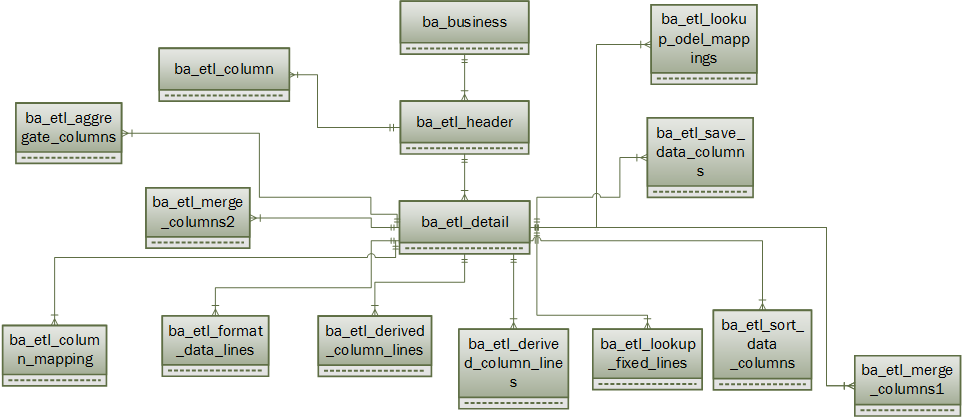
\includegraphics[scale=0.6]{Gambar/Pemodelan-Basisdata}
	\caption{Struktur tabel BI \textit{tool}}
	\end{figure}

Berikut ini penjelasan mengenai pemodelan basisdata dari BI \textit{tool}
\begin{enumerate}
	\item \textbf{ba\_bussiness} : Tujuan pembuatan tabel ini adalah supaya banyak perusahaan/bisnis yan dapat menggunakan \textit{tool} ini (\textit{multicompany/multiclient}).
	\item \textbf{ba\_etl\_header} : Berfungsi sebagai list proses ETL yang ada di bawah perusahaan tersebut.
	\item \textbf{ba\_etl\_detail} : Menyimpan detil setiap proses ETL di bawah perusahaan tersebut.
	\item \textbf{ba\_etl\_columns}: Kolom-kolom yang terlibat di dalam proses ETL, baik dari \textit{file} sumber data maupun yang ditambahkan di tengah proses.
	\item \textbf{ba\_etl\_columns\_mapping} : Detil \textit{mapping} kolom dari data \textit{input} ke \textit{output}. Dimana user bisa memilih untuk tetap memakai nama kolom lama atau mengubahnya.
	\item \textbf{ba\_etl\_format\_data\_lines} : Khusus tipe ETL \textit{format} data menyimpan detil informasi, tipe, dll dari setiap kolom.
	\item \textbf{ba\_etl\_sort\_data\_columns} : Khusus tipe ETL \textit{sort data} menyimpan detil informasi kolom dan arah sorting.
	\item \textbf{ba\_etl\_derived\_column\_lines} : Khusus tipe ETL \textit{derived column} menyimpan detil formula untuk menghasilkan \textit{derived column}.
	\item \textbf{ba\_etl\_lookup\_fixed\_lines} : Khusus tipe ETL \textit{lookup} menyimpan bila \textit{lookup} diambil dari himpunan pilihan \textit{fixed}, tabel ini menampung piluhan-pilihan tersebut.
	\item \textbf{ba\_etl\_save\_data\_columns} : Khusus tipe ETL \textit{save data} menyimpan \textit{mapping} kolom antara hasil dari proses ETL dengan \textit{field} di tabel.
	\item \textbf{ba\_etl\_lookup\_model\_mappings} : Khusus tipe ETL \textit{lookup} menyimpan bila lookup diambil dari tabel lain, tabel ini menampung pasangan \textit{field} di data proses dengan yang di tabel \textit{lookup}.
	\item \textbf{ba\_etl\_merge\_columns1} : Khusus tipe ETL \textit{merge} menyimpan informasi \textit{merge} dari sumber pertama.
	\item \textbf{ba\_etl\_merge\_columns2} : Khusus tipe ETL \textit{merge} menyimpan informasi merge dari sumber kedua
	\item \textbf{ba\_etl\_aggreagate\_columns} : Khusus tipe ETL \textit{aggregate} menyimpan detil informasi proses \textit{aggregate} 
	
\end{enumerate}




















	
}{}
\ifdefstring{\vbabd}{1}{\chapter{Perancangan}
\label{chap:design}
Berdasarkan analisis pada Bab 3, pada bab ini akan dipaparkan mengenai perancangan lojik basisdata, perancangan fisik basisdata, perancangan kelas MVC pada ODOO, diagram kelas, perancangan antar muka BI \textit{tool}, rancangan \textit{method-method} utama.

\section{Perancangan Lojik Basisdata}
Setelah pada bab 3 dijelaskan mengenai pemodelan basis data BI \textit{tool}, pada bagian ini akan digambarkan secara jelas rancangan struktur basisdata dari BI \textit{tool}. Rancangan basisdata ini merupakan impementasi dari skema \textit{star} menempatkan ba\_etl\_detail sebagai \textit{fact table}.\\
Keuntungan menerapkan skema \textit{star} adalah : 
\begin{enumerate}
	\item Lebih mudah dipahami sehingga memudahkan pengguna jika ingin mengembangkan BI \textit{tool} ini lebih lanjut.
	\item Secara teknis memudahkan \textit{developer} jika ingin mengembangkan fitur baru pada BI \textit{tool} ini.
	\item Efisien dalam mengakses data sehingga memudahkan untuk menampilkannya.
\end{enumerate}


\begin{figure}[H]
	\centering
	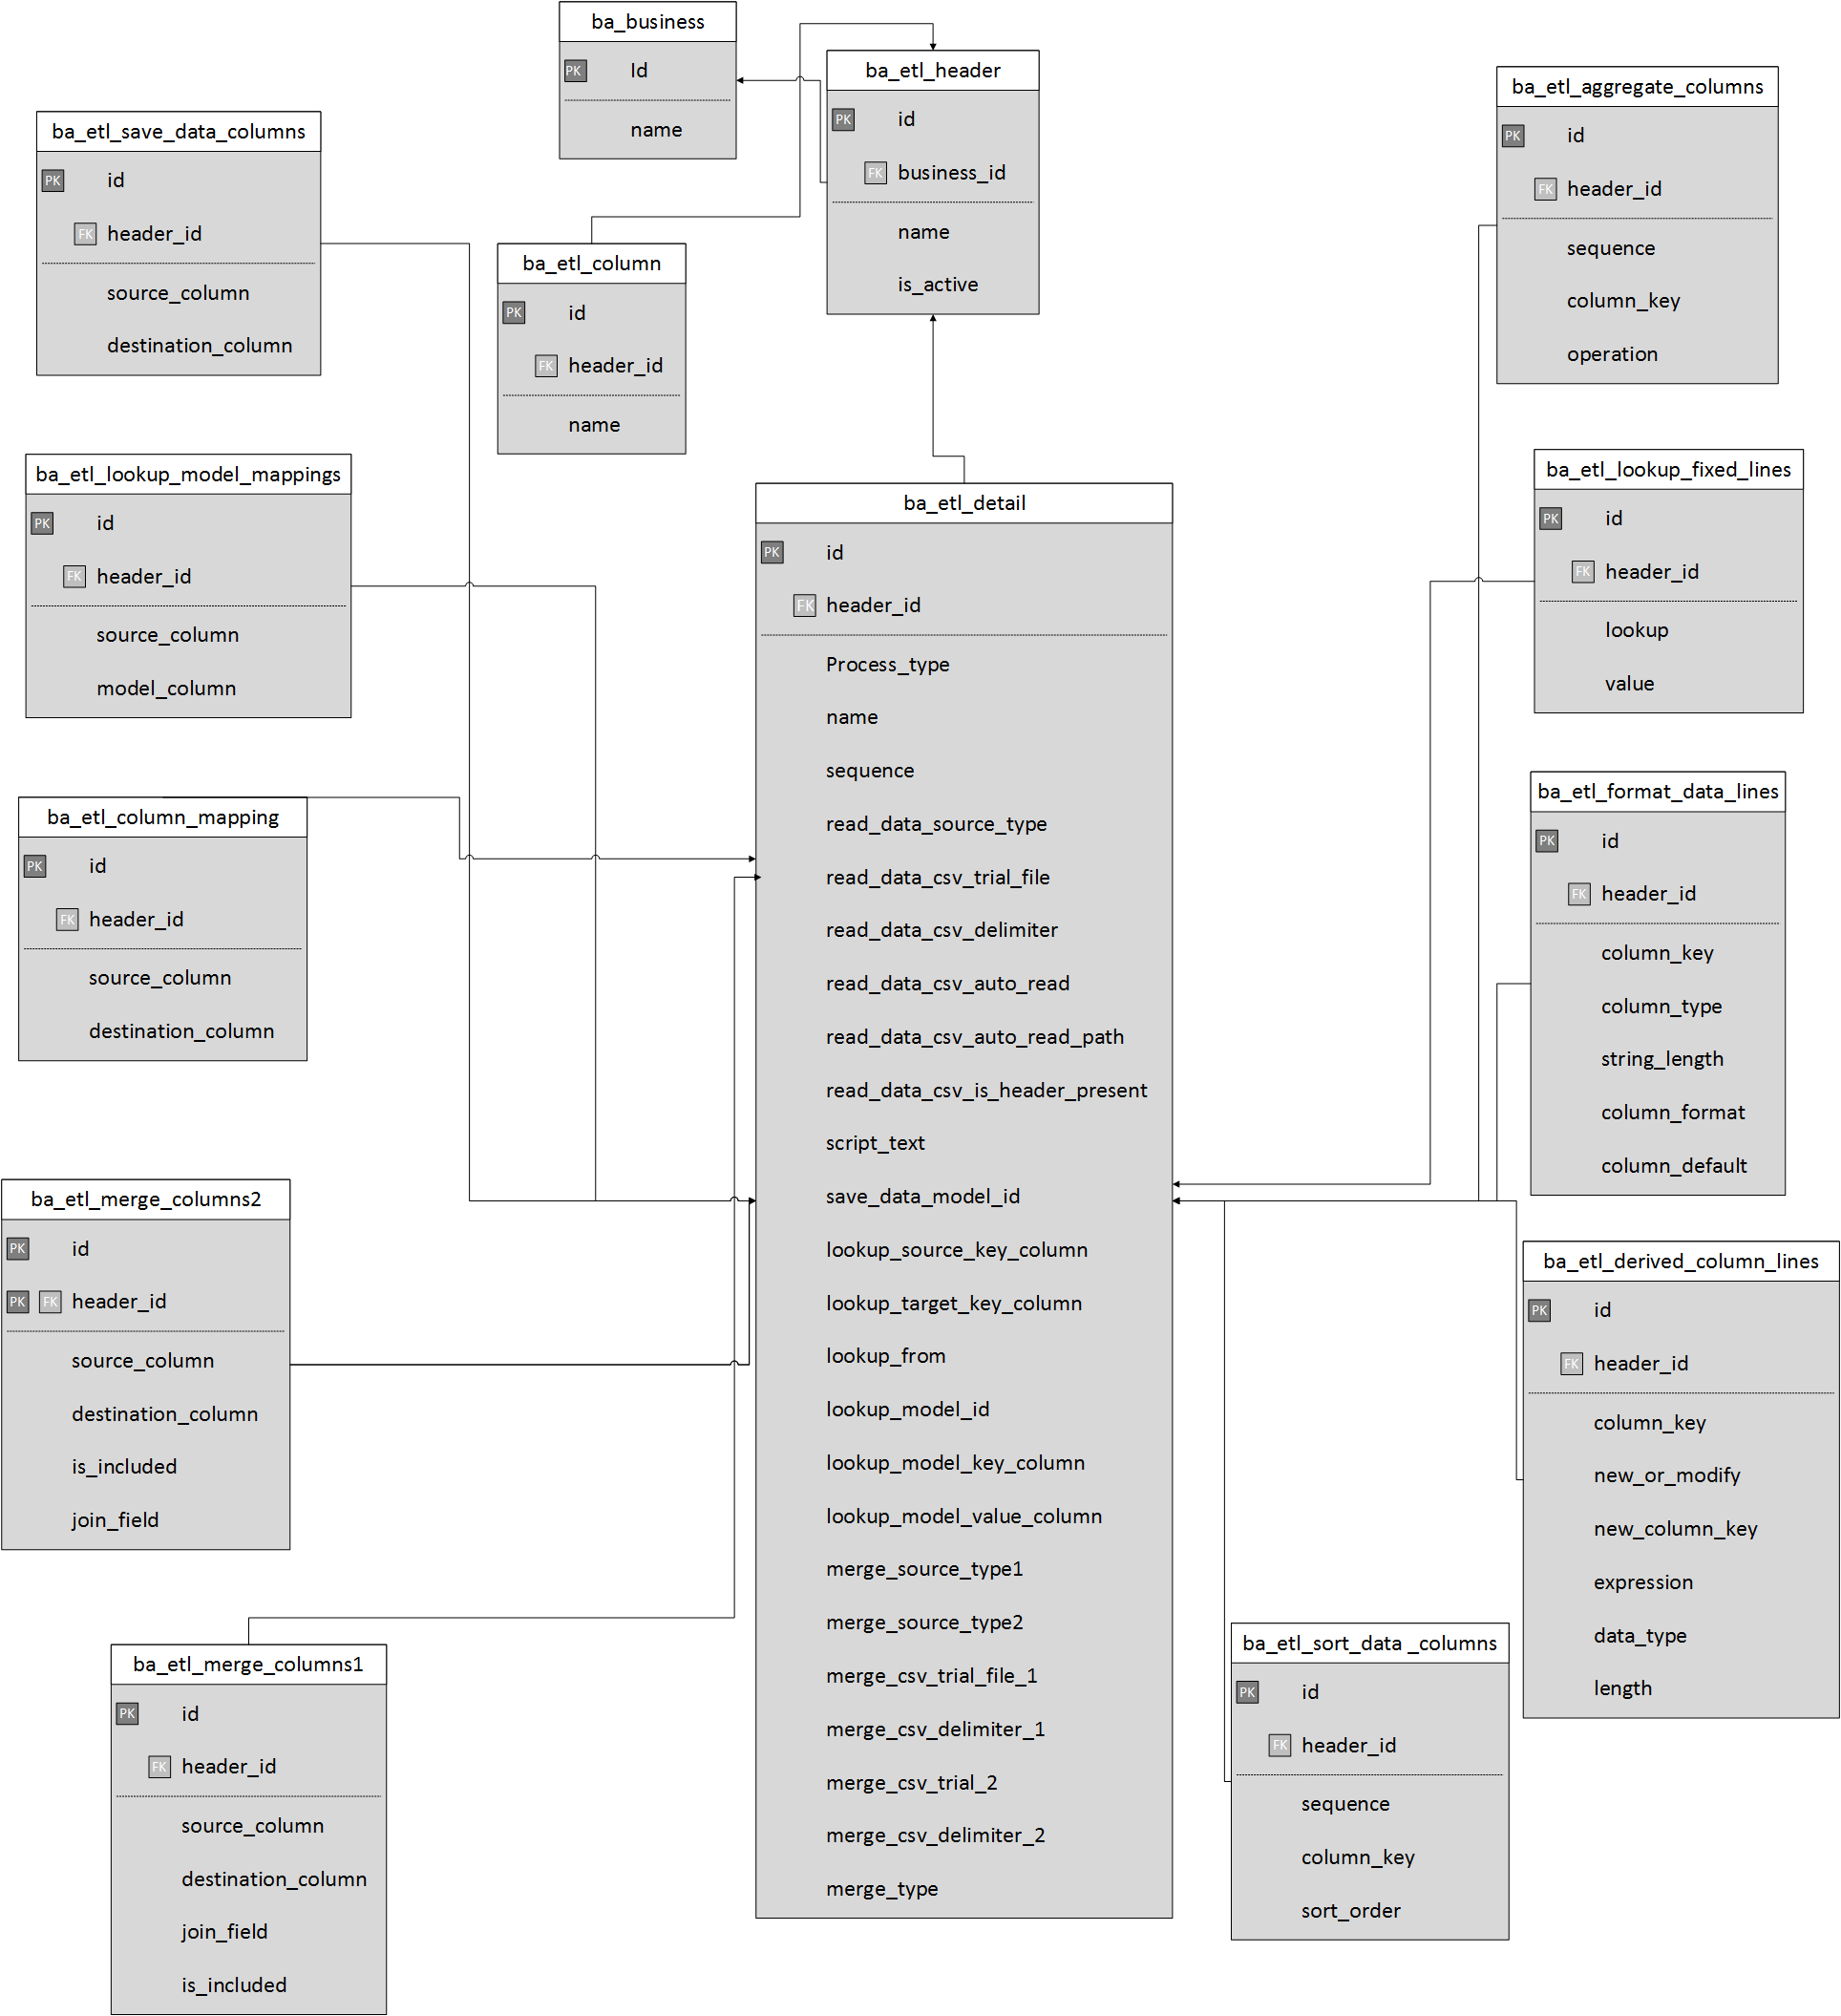
\includegraphics[scale=0.3]{Gambar/rancangan-basisdata-bi}
	\caption{Diagram Relational pada Basisdata BI \textit{tool}}
	\end{figure}
	
	\section{Perancangan Fisik Basisdata}
	Pada bagian sebelumnya telah digambarkan rancangan lojik basisdata BI \textit{tool}, berikut ini penjelasan detil kolom-kolom dalam tabel tersebut.
	\begin{table}[H]
	\centering
		\caption{Tabel \textit{ba\_bussiness}}
		\begin{tabular}{ | c | c| c | c | }
			\hline
				Field & Tipe & Panjang & Constraint \\ \hline \hline
			id & NUMBER & 10 & NOT NULL; PRIMARY KEY  \\ \hline
			name & VARCHAR & 200 & NOT NULL  \\ 		\hline 
		\end{tabular}
\end{table}

\begin{table}[H]
	\centering
		\caption{Tabel \textit{ba\_etl\_header}}
		\begin{tabular}{ | c | p{4cm} | c | p{4cm} |}
			\hline
				Field & Tipe & Panjang & Constraint \\ \hline \hline
			id & NUMBER & 10 & NOT NULL; PRIMARY KEY  \\ \hline
			bussiness\_id & MANY2ONE ba\_business& & NOT NULL; FOREIGN KEY  \\ \hline 
			name & VARCHAR & 200 & NOT NULL \\ \hline 
			is\_active & BOOLEAN &  & DEFAULT TRUE  \\ \hline 
		\end{tabular}
\end{table}

\begin{table}[H]
	\centering
		\caption{Tabel \textit{ba\_etl\_detail}}
		\begin{tabular}{ |c|p{3cm}|c|p{3cm}| }
			\hline
				Field & Tipe & Panjang & Constraint \\ \hline \hline
			id & NUMBER & 10 & NOT NULL; PRIMARY KEY  \\ \hline
			header\_id & MANY2ONE ba\_etl\_header& & NOT NULL; FOREIGN KEY \\ \hline 
			process\_type & ENUM(read\_data, format\_data, lookup, sort\_data, derived\_column, script, merge, aggregate, sort\_data, save\_data)&  & NOT NULL \\ \hline 
			name & VARCHAR &  & NOT NULL \\ \hline 
			sequence & INTEGER &  & NOT NULL  \\ \hline 
			read\_data\_source\_type & ENUM(CSV) & 20 & \\ \hline
			read\_data\_csv\_trial\_file & BINARY &  & \\ \hline 
			read\_data\_csv\_delimiter & VARCHAR & 2 & \\ \hline 
			read\_data\_csv\_auto\_read & BOOLEAN &  & \\ \hline 
			read\_data\_csv\_auto\_read\_path & VARCHAR &  & \\ \hline 
			read\_data\_csv\_is\_header\_present & BOOLEAN &  & DEFAULT TRUE \\ \hline 
			script\_text & TEXT &  & \\ \hline 
			save\_data\_model\_id & MANY2ONE ir\_model &  & \\ \hline 
			lookup\_source\_key\_column & MANY2ONE ba\_etl\_columns &  & \\ \hline
			lookup\_target\_key\_column & varchar & 64 & \\ \hline
			lookup\_from & ENUM(fixed, existing\_table) &  & \\ \hline
			lookup\_model\_id & MANY2ONE ir\_model &  & \\ \hline
			lookup\_model\_key\_column & VARCHAR & 64 & \\ \hline
			lookup\_model\_value\_column & VARCHAR & 64 & \\ \hline
			merge\_source\_type\_1 & ENUM(CSV) &  & \\ \hline
			merge\_source\_type\_2 & ENUM(CSV) &  & \\ \hline
			merge\_csv\_trial\_file\_1 & BINARY &  & \\ \hline
			merge\_csv\_trial\_file\_2 & BINARY &  & \\ \hline
			merge\_csv\_delimiter\_1 & VARCHAR & 3 & \\ \hline
			merge\_csv\_delimiter\_2 & VARCHAR & 3 & \\ \hline
			merge\_type & ENUM(left, right, inner) &  & \\ \hline
		\end{tabular}
\end{table}

\begin{table}[H]
	\centering
		\caption{Tabel \textit{ba\_etl\_columns}}
		\begin{tabular}{ | c | p{4cm} | c | p{4cm} |}
			\hline
				Field & Tipe & Panjang & Constraint \\ \hline \hline
			id & NUMBER & 10 & NOT NULL; PRIMARY KEY  \\ \hline
			header\_id & MANY2ONE ba\_etl\_header & &  FOREIGN KEY  \\ \hline 
			name & VARCHAR & 64 & \\ \hline 
		\end{tabular}
\end{table}

\begin{table}[H]
	\centering
		\caption{Tabel \textit{ba\_etl\_columns\_mapping}}
		\begin{tabular}{ | c | p{4cm} | c | p{4cm} |}
			\hline
				Field & Tipe & Panjang & Constraint \\ \hline \hline
			id & NUMBER & 10 & NOT NULL; PRIMARY KEY  \\ \hline
			header\_id & MANY2ONE ba\_etl\_detail & & NOT NULL; FOREIGN KEY  \\ \hline 
			source\_column & VARCHAR & 64 &  \\ \hline 
			detination\_column & VARCHAR & 64 &  \\ \hline 
		\end{tabular}
\end{table}

\begin{table}[H]
	\centering
		\caption{Tabel \textit{ba\_etl\_format\_data\_lines}}
		\begin{tabular}{ | c | p{4cm} | c | p{4cm} |}
			\hline
				Field & Tipe & Panjang & Constraint \\ \hline \hline
			id & NUMBER & 10 & NOT NULL; PRIMARY KEY  \\ \hline
			header\_id & MANY2ONE ba\_etl\_detail & & NOT NULL; FOREIGN KEY  \\ \hline 
			column\_key & MANY2ONE ba\_etl\_columns &  & NOT NULL  \\ \hline 
			column\_type & ENUM(char, integer, float, date, datetime, boolean, selection) &  &  \\ \hline 
		string\_length & INTEGER &  &  \\ \hline
		column\_format & VARCHAR & 50 &  \\ \hline
		column\_default & VARCHAR & 500  &  \\ \hline
		\end{tabular}
\end{table}

\begin{table}[H]
	\centering
		\caption{Tabel \textit{ba\_etl\_sort\_data\_columns}}
		\begin{tabular}{ | c | p{4cm} | c | p{4cm} |}
			\hline
				Field & Tipe & Panjang & Constraint \\ \hline \hline
			id & NUMBER & 10 & NOT NULL; PRIMARY KEY  \\ \hline
			header\_id & MANY2ONE ba\_etl\_detail & & NOT NULL; FOREIGN KEY  \\ \hline 
			sequence & INTEGER &  & NOT NULL  \\ \hline 
			column\_key & MANY2ONE ba\_etl\_columns &  &  \\ \hline 
		sort\_order & ENUM(asc, desc) &  & DEFAULT ASC  \\ \hline
		\end{tabular}
\end{table}

\begin{table}[H]
	\centering
		\caption{Tabel \textit{ba\_etl\_derived\_column\_lines}}
		\begin{tabular}{ | c | p{4cm} | c | p{4cm} |}
			\hline
				Field & Tipe & Panjang & Constraint \\ \hline \hline
			id & NUMBER & 10 & NOT NULL; PRIMARY KEY  \\ \hline
			header\_id & MANY2ONE ba\_etl\_detail & & NOT NULL; FOREIGN KEY  \\ \hline 	
			column\_key & MANY2ONE ba\_etl\_columns &  &   \\ \hline
			new\_or\_modify  & ENUM(new, modify) &  & DEFAULT NEW\\ \hline
			new\_column\_key & VARCHAR & 64 &  \\ \hline 
		expression & TEXT &  &  \\ \hline
		data\_type & ENUM(char, integer, float, date, datetime, boolean, selection) & &  \\ \hline
		length & INTEGER &   &  \\ \hline
		\end{tabular}
\end{table}

\begin{table}[H]
	\centering
		\caption{Tabel \textit{ba\_etl\_lookup\_fixed\_lines}}
		\begin{tabular}{ | c | p{4cm} | c | p{4cm} |}
			\hline
				Field & Tipe & Panjang & Constraint \\ \hline \hline
			id & NUMBER & 10 & NOT NULL; PRIMARY KEY  \\ \hline
			header\_id & MANY2ONE ba\_etl\_detail & & NOT NULL; FOREIGN KEY  \\ \hline 
			lookup & VARCHAR & 500  &  \\ \hline 
			value & VARCHAR & 500  &  \\ \hline 
		\end{tabular}
\end{table}

\begin{table}[H]
	\centering
		\caption{Tabel \textit{ba\_etl\_save\_data\_column}}
		\begin{tabular}{ | c | p{4cm} | c | p{4cm} |}
			\hline
				Field & Tipe & Panjang & Constraint \\ \hline \hline
			id & NUMBER & 10 & NOT NULL; PRIMARY KEY  \\ \hline
			header\_id & MANY2ONE ba\_etl\_detail & & \\ \hline 
			source\_column & MANY2ONE ba\_etl\_column & &  \\ \hline 
			destination\_column & VARCHAR & 64  &  \\ \hline  
		\end{tabular}
\end{table}

\begin{table}[H]
	\centering
		\caption{Tabel \textit{ba\_etl\_lookup\_model\_mappings}}
		\begin{tabular}{ | c | p{4cm} | c | p{4cm} |}
			\hline
				Field & Tipe & Panjang & Constraint \\ \hline \hline
			id & NUMBER & 10 & NOT NULL; PRIMARY KEY  \\ \hline
			header\_id & MANY2ONE ba\_etl\_detail & & \\ \hline 
			source\_column & MANY2ONE ba\_etl\_column & &  \\ \hline 
			destination\_column & VARCHAR & 64  &  \\ \hline  
		\end{tabular}
\end{table}

\begin{table}[H]
	\centering
		\caption{Tabel \textit{ba\_etl\_merge\_columns\_1}}
		\begin{tabular}{ | c | p{4cm} | c | p{4cm} |}
			\hline
				Field & Tipe & Panjang & Constraint \\ \hline \hline
			id & NUMBER & 10 & NOT NULL; PRIMARY KEY  \\ \hline
			header\_id & MANY2ONE ba\_etl\_detail & & \\ \hline 
			source\_column & VARCHAR & 64 &  \\ \hline 
			destination\_column & VARCHAR & 64  &  \\ \hline
			is\_included & BOOLEAN &  & DEFAULT 1 \\ \hline
			join\_field & VARCHAR & 64  &  \\ \hline
		\end{tabular}
\end{table}

\begin{table}[H]
	\centering
		\caption{Tabel \textit{ba\_etl\_merge\_columns\_2}}
		\begin{tabular}{ | c | p{4cm} | c | p{4cm} |}
			\hline
				Field & Tipe & Panjang & Constraint \\ \hline \hline
			id & NUMBER & 10 & NOT NULL; PRIMARY KEY  \\ \hline
			header\_id & MANY2ONE ba\_etl\_detail & & \\ \hline 
			source\_column & VARCHAR & 64 &  \\ \hline 
			destination\_column & VARCHAR & 64  &  \\ \hline
			is\_included & BOOLEAN &  & DEFAULT 1 \\ \hline
			join\_field & VARCHAR & 64  &  \\ \hline
		\end{tabular}
\end{table}

\begin{table}[H]
	\centering
		\caption{Tabel \textit{ba\_etl\_aggregate\_columns}}
		\begin{tabular}{ | c | p{4cm} | c | p{4cm} |}
			\hline
				Field & Tipe & Panjang & Constraint \\ \hline \hline
			id & NUMBER & 10 & NOT NULL; PRIMARY KEY  \\ \hline
			header\_id & MANY2ONE ba\_etl\_detail & & \\ \hline 
			sequence & INTEGER &  &  \\ \hline 
			column\_key & MANY2ONE ba\_etl\_columns &  &  \\ \hline
			operation & ENUM(none, count, sum, avg, max, min, group\_by) &  &\\ \hline
		\end{tabular}
\end{table}

\section{Diagram Kelas}
Berikut ini merupakan gambaran diagram kelas dari BI \textit{tool}. Setiap kelas pada diagram ini meng-\textit{extend} kelas osv yang merupakan bawaan dari \textit{framework} ODOO.

\begin{figure}[h]
	\centering
	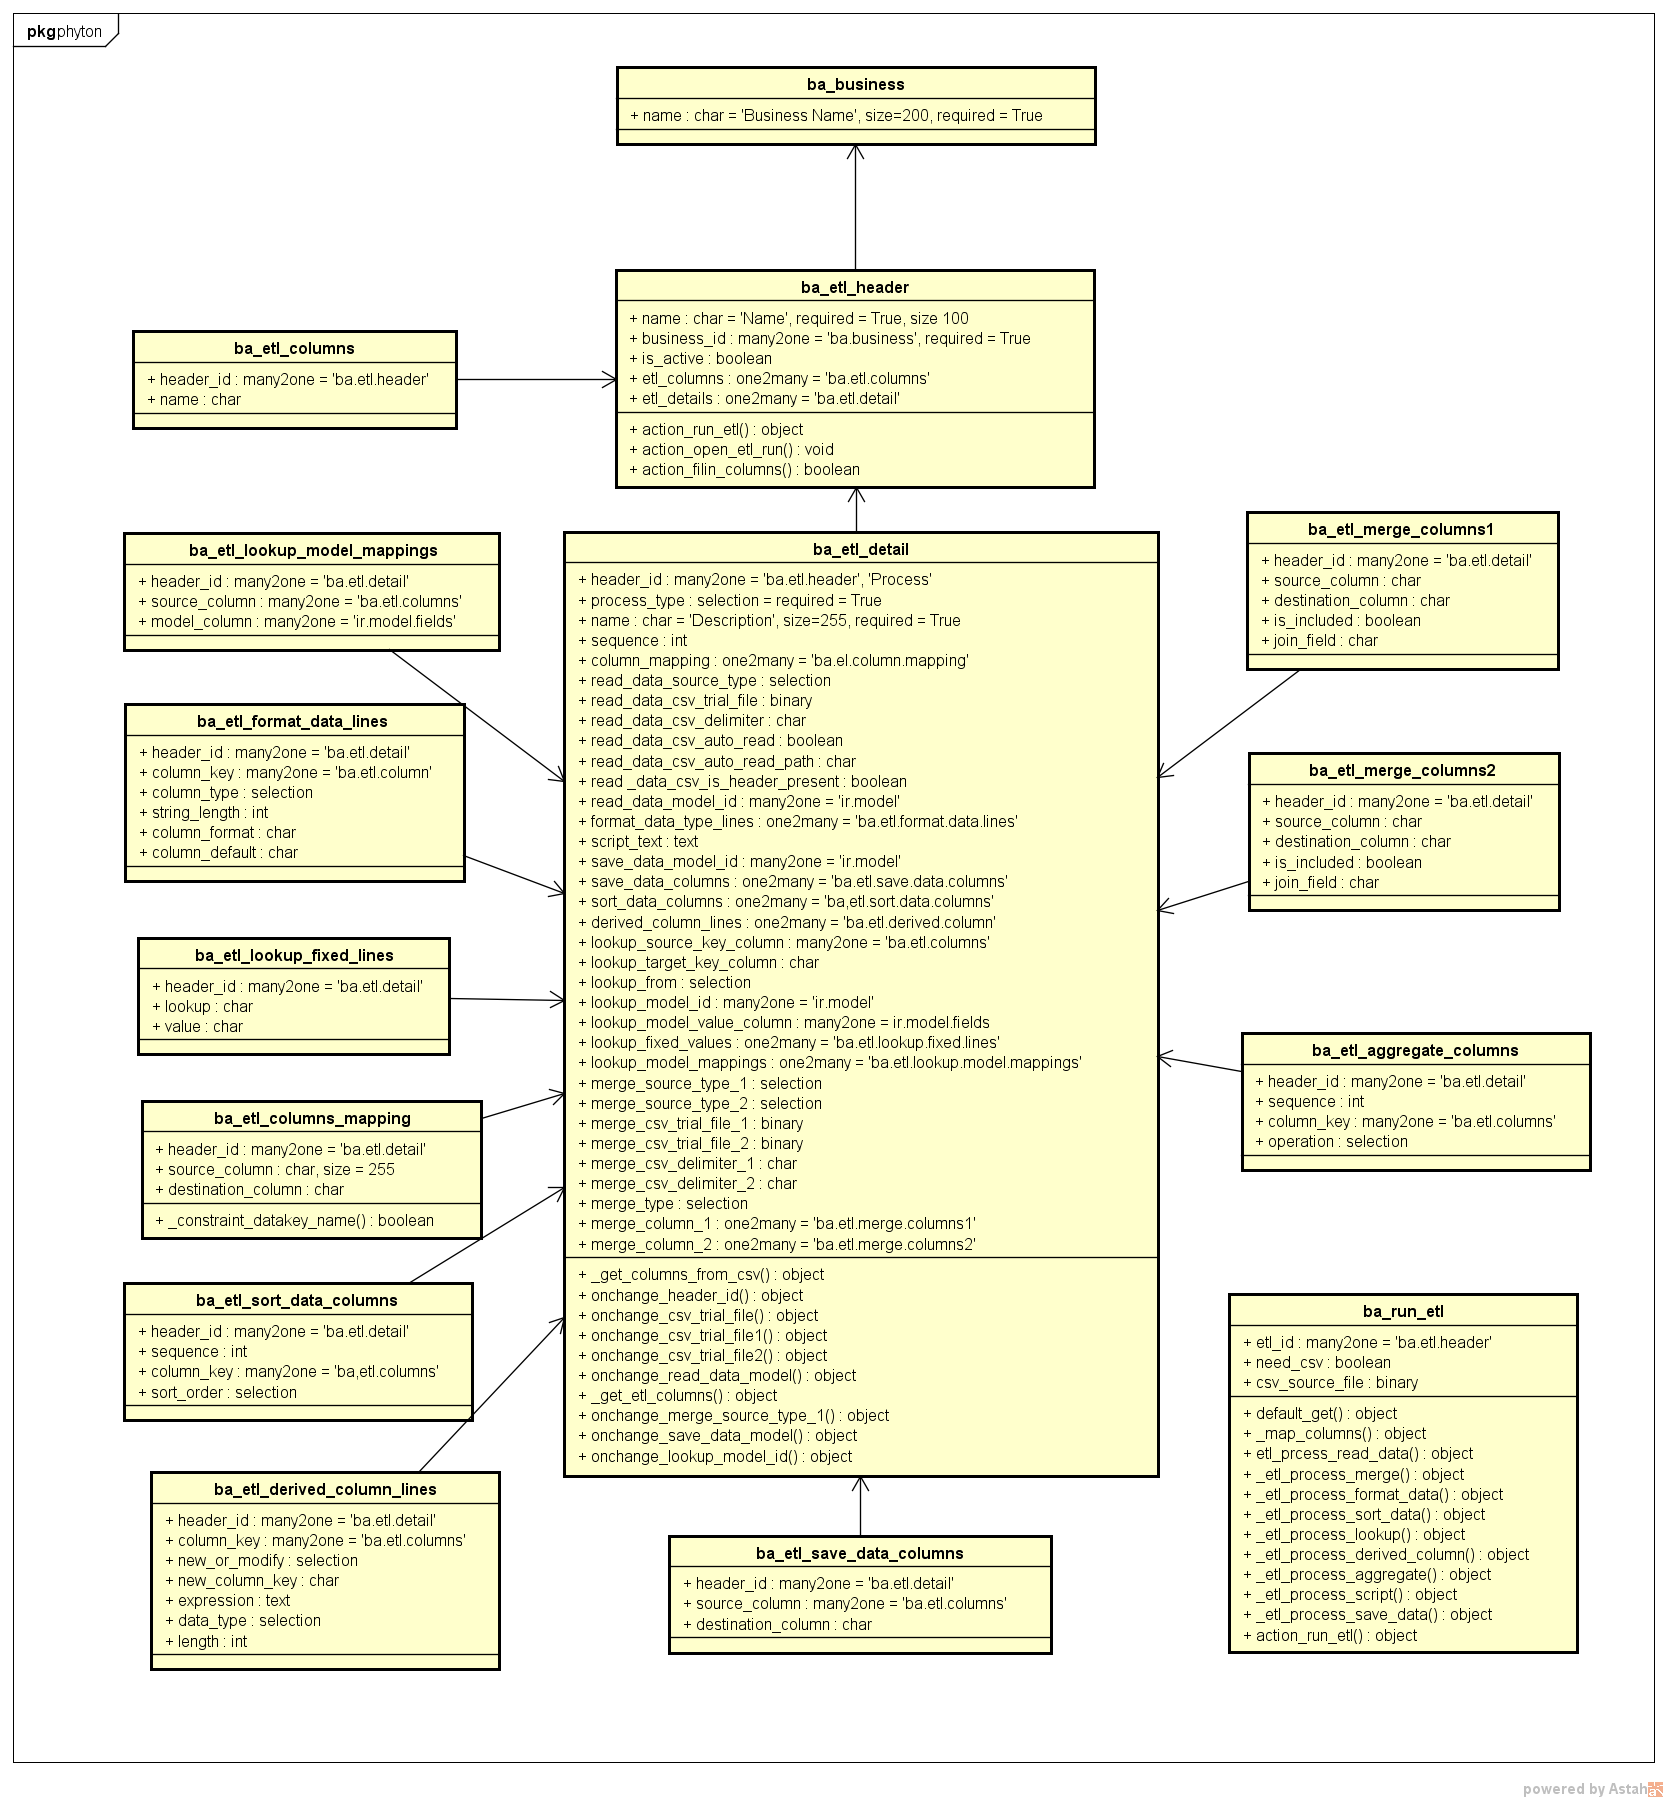
\includegraphics[scale=0.4]{Gambar/Class-Diagram-bi-tool}
	\caption{Struktur kelas diagram BI \textit{tool}}
	\end{figure}
	
	
	\begin{table}[H]
	\centering
		\caption{Tabel Kelas \textit{ba\_bussiness}}
		\begin{tabular}{ | c | c|}
			\hline
				\multicolumn{2}{|c|}{Atribut}\\ \hline 
				Nama atribut & Tipe Data\\ \hline
			name & CHAR(200)\\ \hline
		\end{tabular}
\end{table}

\begin{table}[H]
	\centering
		\caption{Tabel Kelas \textit{ba\_etl\_header}}
		\begin{tabular}{ | c | c|}
			\hline
				\multicolumn{2}{|c|}{Atribut}\\ \hline 
				Nama atribut & Tipe Data\\ \hline
			name & CHAR(100)\\ \hline
			business\_id & MANY2ONE('ba.business')\\ \hline
			is\_active & BOOLEAN\\ \hline
			etl\_columns & ONE2MANY('ba.etl.columns')\\ \hline
			etl\_detail & ONE2MANY('ba.etl.detail')\\ \hline
			\multicolumn{2}{|c|}{Method}\\ \hline 
			\multicolumn{2}{|l|}{action\_run\_etl()}\\ \hline 
			\multicolumn{2}{|l|}{action\_open\_etl\_run()}\\ \hline
			\multicolumn{2}{|l|}{action\_fillin\_columns()}\\ \hline
		\end{tabular}
\end{table}

\begin{table}[H]
	\centering
		\caption{Tabel Kelas \textit{ba\_etl\_columns}}
		\begin{tabular}{ | c | c|}
			\hline
				\multicolumn{2}{|c|}{Atribut}\\ \hline 
				Nama atribut & Tipe Data\\ \hline
			header\_id & MANY2ONE('ba.etl.header')\\ \hline
			name & CHAR\\ \hline
		\end{tabular}
\end{table}

\begin{table}[H]
	\centering
		\caption{Tabel Kelas \textit{ba\_etl\_detail}}
		\begin{tabular}{ | c | c|}
			\hline
				\multicolumn{2}{|c|}{Atribut}\\ \hline 
				Nama atribut & Tipe Data\\ \hline
			header\_id & MANY2ONE('ba.etl.header')\\ \hline
			process\_type & selection\\ \hline
			name & CHAR(255)\\ \hline
			sequence &  INT\\ \hline
			column\_mapping &  ONE2MANY('ba.el.column.mapping)\\ \hline
			read\_data\_source\_type & SELECTION\\ \hline
			read\_data\_csv\_trial\_file &  BINARY\\ \hline
			read\_data\_csv\_delimiter &  CHAR\\ \hline
			read\_data\_csv\_auto\_read &  BOOLEAN\\ \hline
			read\_data\_csv\_auto\_read\_path &  CHAR\\ \hline
			read\_data\_csv\_is\_header\_present &  BOOLEAN\\ \hline
			read\_data\_model\_id &  MANY2ONE('ir.model')\\ \hline
			format\_data\_type\_lines &  ONE2MANY('ba.etl.format.data.lines')\\ \hline
			script\_text &  TEXT\\ \hline
			save\_data\_model\_id &  MANY2ONE('ir.model')\\ \hline
			save\_data\_columns & ONE2MANY('ba.etl.save.data.columns')\\ \hline
			sort\_data\_columns &  ONE2MANY('ba.etl.sort.data.column')\\ \hline
			 derived\_column\_lines &  ONE2MANY('ba.etl.derived.column')\\ \hline
			lookup\_source\_key\_column &  MANY2ONE('ba.etl.columns')\\ \hline
			lookup\_target\_key\_column &  CHAR\\ \hline
			lookup\_from &  SELECTION\\ \hline
		  lookup\_model\_id &  MANY2ONE('ir.model')\\ \hline
			lookup\_model\_value\_column &  MANY2ONE(ir.model.fields)\\ \hline
			lookup\_fixed\_values &  ONE2MANY('ba.etl.lookup.fixed.lines')\\ \hline
			lookup\_model\_mappings &  ONE2MANY('ba.etl.lookup.model.mappings')\\ \hline
			merge\_source\_type\_1 &  SELECTION\\ \hline
			merge\_source\_type\_2 &  SELECTION\\ \hline
			merge\_csv\_trial\_file\_1 &  BINARY\\ \hline
			merge\_csv\_trial\_file\_2 &  BINARY\\ \hline
			merge\_csv\_delimiter\_1 &  CHAR\\ \hline
			merge\_csv\_delimiter\_2 &  CHAR\\ \hline
			merge\_type &  SELECTION\\ \hline
			merge\_column\_1 &  ONE2MANY('ba.etl.merge.columns1')\\ \hline
			merge\_column\_2 &  ONE2MANY('ba.etl.merge.columns2')\\ \hline
			\multicolumn{2}{|c|}{Method}\\ \hline 
			\multicolumn{2}{|l|}{get\_columns\_from\_csv(csv\_content, delimiter) }\\ \hline 
			\multicolumn{2}{|l|}{onchange\_header\_id(header\_id)}\\ \hline
			\multicolumn{2}{|l|}{onchange\_csv\_trial\_file(read\_data\_csv\_trial\_file, delimiter)}\\ \hline
			\multicolumn{2}{|l|}{onchange\_csv\_trial\_file1(merge\_csv\_trial\_file\_1, merge\_csv\_delimiter\_1)}\\ \hline
			\multicolumn{2}{|l|}{onchange\_csv\_trial\_file2(merge\_csv\_trial\_file\_2, merge\_csv\_delimiter\_2)}\\ \hline
			\multicolumn{2}{|l|}{onchange\_read\_data\_model(read\_data\_model\_id)}\\ \hline
			\multicolumn{2}{|l|}{get\_etl\_columns(header\_id)}\\ \hline
			\multicolumn{2}{|l|}{onchange\_merge\_source\_type\_1(header\_id, merge\_source\_type\_1)}\\ \hline
			\multicolumn{2}{|l|}{onchange\_save\_data\_model(save\_data\_model\_id)}\\ \hline
			\multicolumn{2}{|l|}{onchange\_lookup\_model\_id(lookup\_model\_id)}\\ \hline
			
		\end{tabular}
\end{table}

\begin{table}[H]
	\centering
		\caption{Tabel Kelas \textit{ba\_etl\_columns\_mapping}}
		\begin{tabular}{ | c | c|}
			\hline
				\multicolumn{2}{|c|}{Atribut}\\ \hline 
				Nama atribut & Tipe Data\\ \hline
				header\_id & MANY2ONE('ba.etl.detail')\\ \hline
				source\_column & CHAR(255)\\ \hline
				destination\_column & CHAR\\ \hline
				\multicolumn{2}{|c|}{Method}\\ \hline
				\multicolumn{2}{|l|}{constraint\_datakey\_name()}
		\end{tabular}
\end{table}
	
	\begin{table}[H]
	\centering
		\caption{Tabel Kelas \textit{ba\_etl\_format\_data\_lines}}
		\begin{tabular}{ | c | c|}
			\hline
				\multicolumn{2}{|c|}{Atribut}\\ \hline 
				Nama atribut & Tipe Data\\ \hline
				header\_id & MANY2ONE('ba.etl.detail')\\ \hline
				column\_key & MANY2ONE('ba.etl.column')\\ \hline
				column\_type & SELECTION\\ \hline
				string\_length & INT\\ \hline
				column\_format & CHAR(50)\\ \hline
				column\_default & CHAR(500)\\ \hline
		\end{tabular}
\end{table}

\begin{table}[H]
	\centering
		\caption{Tabel Kelas \textit{ba\_etl\_sort\_data\_columns}}
		\begin{tabular}{ | c | c|}
			\hline
				\multicolumn{2}{|c|}{Atribut}\\ \hline 
				Nama atribut & Tipe Data\\ \hline
				header\_id & MANY2ONE('ba.etl.detail')\\ \hline
				sequence & INT\\ \hline
				column\_key & MANY2ONE('ba.etl.column')\\ \hline
				sort\_order & SELECTION\\ \hline
		\end{tabular}
\end{table}

\begin{table}[H]
	\centering
		\caption{Tabel Kelas \textit{ba\_etl\_derived\_column\_lines}}
		\begin{tabular}{ | c | c|}
			\hline
				\multicolumn{2}{|c|}{Atribut}\\ \hline 
				Nama atribut & Tipe Data\\ \hline
				header\_id & MANY2ONE('ba.etl.detail')\\ \hline
				column\_key & MANY2ONE('ba.etl.column')\\ \hline
				new\_or\_modify  & SELECTION\\ \hline
				new\_column\_key & CHAR(64)\\ \hline
				expression & TEXT \\ \hline
				data\_type & SELECTION \\ \hline
				length & INT \\ \hline
		\end{tabular}
\end{table}

\begin{table}[H]
	\centering
		\caption{Tabel Kelas \textit{ba\_etl\_save\_data\_columns}}
		\begin{tabular}{ | c | c|}
			\hline
				\multicolumn{2}{|c|}{Atribut}\\ \hline 
				Nama atribut & Tipe Data\\ \hline
				header\_id & MANY2ONE('ba.etl.detail')\\ \hline
				source\_column & MANY2ONE('ba.etl.column')\\ \hline
				destination & CHAR(64)\\ \hline
		\end{tabular}
\end{table}

\begin{table}[H]
	\centering
		\caption{Tabel Kelas \textit{ba\_etl\_lookup\_fixed\_lines}}
		\begin{tabular}{ | c | c|}
			\hline
				\multicolumn{2}{|c|}{Atribut}\\ \hline 
				Nama atribut & Tipe Data\\ \hline
				header\_id & MANY2ONE('ba.etl.detail')\\ \hline
				lookup & CHAR\\ \hline
				value& CHAR\\ \hline
		\end{tabular}
\end{table}

\begin{table}[H]
	\centering
		\caption{Tabel Kelas \textit{ba\_etl\_lookup\_model\_mappings}}
		\begin{tabular}{ | c | c|}
			\hline
				\multicolumn{2}{|c|}{Atribut}\\ \hline 
				Nama atribut & Tipe Data\\ \hline
				header\_id & MANY2ONE('ba.etl.detail')\\ \hline
				source\_column & MANY2ONE('ba.etl.column')\\ \hline
				model\_column & MANY2ONE('ir.model.fields')\\ \hline
		\end{tabular}
\end{table}

\begin{table}[H]
	\centering
		\caption{Tabel Kelas \textit{ba\_etl\_merge\_columns1}}
		\begin{tabular}{ | c | c|}
			\hline
				\multicolumn{2}{|c|}{Atribut}\\ \hline 
				Nama atribut & Tipe Data\\ \hline
				header\_id & MANY2ONE('ba.etl.detail')\\ \hline
				source\_column & CHAR(64)\\ \hline
				destination\_column & CHAR(64)\\ \hline
				is\_included & BOOLEAN\\ \hline
				join\_field & CHAR\\ \hline
		\end{tabular}
\end{table}

\begin{table}[H]
	\centering
		\caption{Tabel Kelas \textit{ba\_etl\_merge\_columns2}}
		\begin{tabular}{ | c | c|}
			\hline
				\multicolumn{2}{|c|}{Atribut}\\ \hline 
				Nama atribut & Tipe Data\\ \hline
				header\_id & MANY2ONE('ba.etl.detail')\\ \hline
				source\_column & CHAR(64)\\ \hline
				destination\_column & CHAR(64)\\ \hline
				is\_included & BOOLEAN\\ \hline
				join\_field & CHAR\\ \hline
		\end{tabular}
\end{table}

\begin{table}[H]
	\centering
		\caption{Tabel Kelas \textit{ba\_etl\_aggregate\_columns}}
		\begin{tabular}{ | c | c|}
			\hline
				\multicolumn{2}{|c|}{Atribut}\\ \hline 
				Nama atribut & Tipe Data\\ \hline
				header\_id & MANY2ONE('ba.etl.detail')\\ \hline
				sequence & INT\\ \hline
				column\_key & MANY2ONE('ba.etl.columns')\\ \hline
				operation & SELECTION\\ \hline
		\end{tabular}
\end{table}

\begin{table}[H]
	\centering
		\caption{Tabel Kelas \textit{ba\_run\_etl}}
		\begin{tabular}{ | c | c|}
			\hline
				\multicolumn{2}{|c|}{Atribut}\\ \hline 
				Nama atribut & Tipe Data\\ \hline
				etl\_id & MANY2ONE('ba.etl.header')\\ \hline
				need\_csv & BOOLEAN\\ \hline
				csv\_source\_file & BINARY\\ \hline
				\multicolumn{2}{|c|}{Method}\\ \hline
				\multicolumn{2}{|l|}{default\_get(fields)}\\ \hline
				\multicolumn{2}{|l|}{map\_columns(source\_data, columns\_mapping)}\\ \hline
				\multicolumn{2}{|l|}{etl\_process\_read\_data(step\_info, raw\_data)}\\ \hline
				\multicolumn{2}{|l|}{etl\_process\_merge(step\_info, raw\_data)}\\ \hline
				\multicolumn{2}{|l|}{etl\_process\_format\_data(step\_info, raw\_data)}\\ \hline
				\multicolumn{2}{|l|}{etl\_process\_sort\_data(step\_info, raw\_data)}\\ \hline
				\multicolumn{2}{|l|}{etl\_process\_lookup(step\_info, raw\_data)}\\ \hline
				\multicolumn{2}{|l|}{etl\_process\_derived\_column(step\_info, raw\_data)}\\ \hline
				\multicolumn{2}{|l|}{etl\_process\_aggregate(step\_info, raw\_data)}\\ \hline
				\multicolumn{2}{|l|}{etl\_process\_script(step\_info, raw\_data)}\\ \hline
				\multicolumn{2}{|l|}{etl\_process\_save\_data(step\_info, raw\_data)}\\ \hline
				\multicolumn{2}{|l|}{action\_run\_etl(etl\_id)}\\ \hline
		\end{tabular}
\end{table}
}{}
\ifdefstring{\vbabe}{1}{\chapter{Implementasi dan Pengujian}
\label{chap:implementation}
Pada bagian ini akan dijelaskan mengenai lingkungan implementasi perangkat keras maupun perangkat lunak. Serta implementasi basisdata BI \textit{tool} beserta tampilan antar muka. Terakhir akan dibahas mengenai pengujian pada perangkat lunak ini.
\section{Lingkungan Implementasi}
\subsection{Lingkungan Perangkat Keras}
Dalam mengembangakan perangkat ini, digunakan spesifikasi perangkat keras sebagai berikut:
\begin{itemize}
	\item \text{Processor} : Intel Core i7 2.4 Ghz
	\item \textit{Memory} : 8 GB
	\item \textit{Hardisk} : 640 GB
	\item VGA : Nvidia GeForce 540M
	\item \textit{keyboard} dan \textit{mouse standard}
\end{itemize}

\subsection{Lingkungan Perangkat Lunak}
Untuk pengembangan perangkat lunak BI \textit{tool}, digunakan spesifikasi sebagai berikut:
\begin{itemize}
	\item \textit{Tools:} ODOO 8.0-20141128
	\item Bahasa Pemograman Phyton 2.7
	\item \textit{Database management system} PosgreSQL 9.3
	\item \textit{Operating system}: windows 8
\end{itemize}

\section{Implementasi Tabel Basisdata}
\subsection{Tabel Basisdata ETL dan Bisnis}
Berikut implementasi tabel basisdata yang terlibat langsung dalam proses ETL beserta pendukungnnya.
\begin{itemize}
	\item Tabel ba\_business\\
	Tabel ini digunakan untuk mencatat semua bisnis yang menggunakan perangkat lunak ini. Selain itu , agar dapat \textit{multicompany/multiclient}.
	
	\begin{figure}[H]
	\centering
	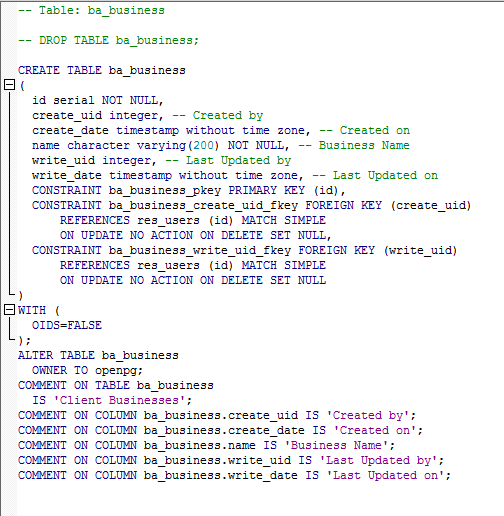
\includegraphics[scale=0.5]{Gambar/tabel-ba-business}
	\caption{Implementasi tabel ba\_business}
	\end{figure}

	\item Tabel ba\_etl\_header\\
	Tabel ini mencatat proses ETL yang ada di bawah perusahaan/bisnis yang ada.
	\begin{figure}[H]
	\centering
	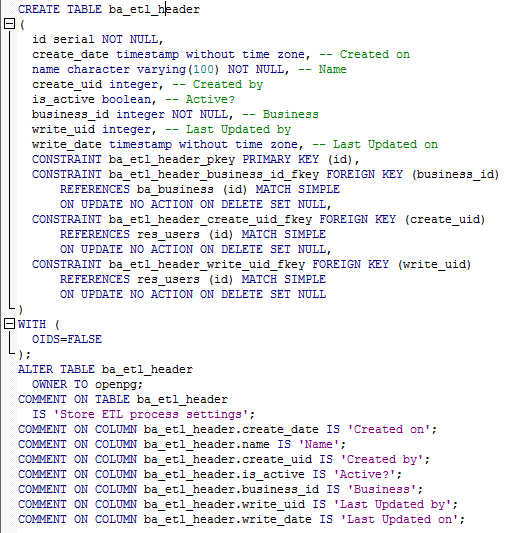
\includegraphics[scale=0.5]{Gambar/tabel-ba-etl-header}
	\caption{Implementasi tabel ba\_etl\_header}
	\end{figure}
	
	\item Tabel ba\_etl\_detail\\
	Tabel ini mencata detail dari setiap proses ETL dibawah perusahaan/bisnis. 
	\begin{figure}[H]
	\centering
	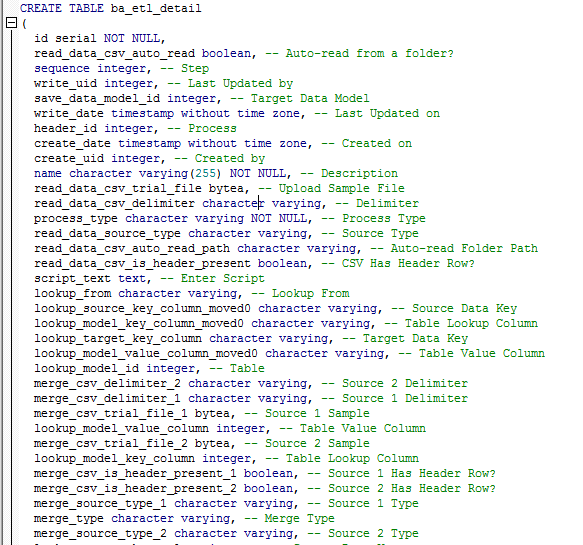
\includegraphics[scale=0.5]{Gambar/tabel-ba-etl-detail}
	\caption{Implementasi tabel ba\_etl\_detail}
	\end{figure}
	
	\begin{figure}[H]
	\centering
	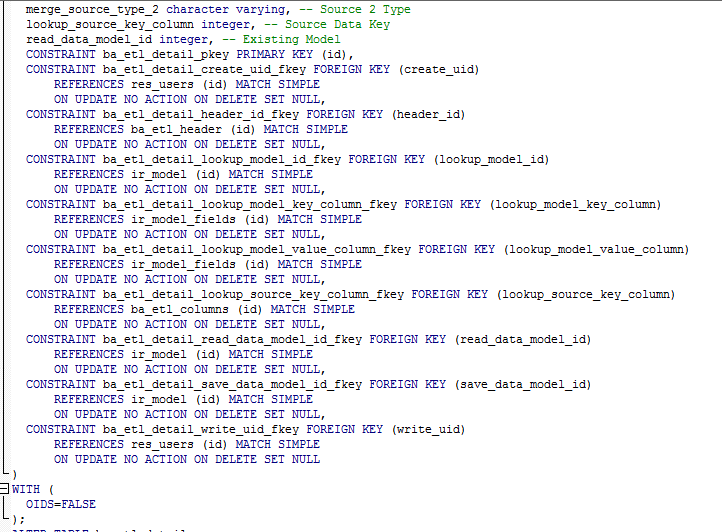
\includegraphics[scale=0.5]{Gambar/tabel-ba-etl-detail2}
	\caption{Implementasi tabel ba\_etl\_detail2}
	\end{figure}

\begin{figure}[H]
	\centering
	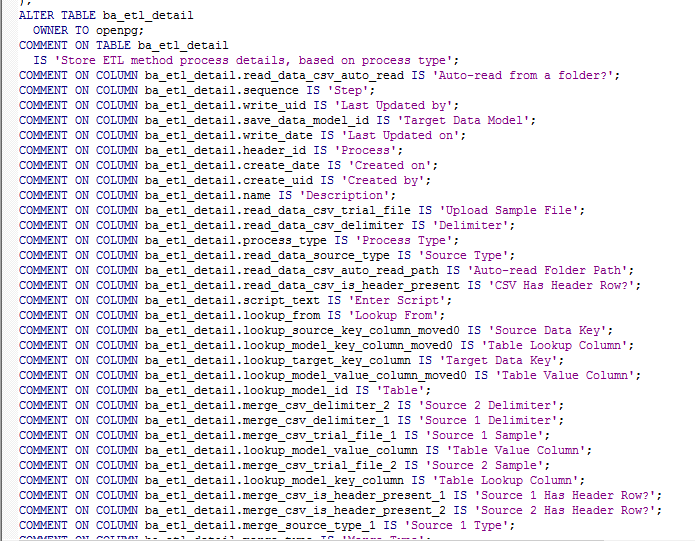
\includegraphics[scale=0.5]{Gambar/tabel-ba-etl-detail3}
	\caption{Implementasi tabel ba\_etl\_detail3}
	\end{figure}

	\item Tabel basisdata ba\_etl\_columns\\
	Tabel ini berfungsi menyimpan kolom-kolom yang terlibat dalam proses ETL, baik dari sumber data maupun yang ditambahkan di tengah proses
	\begin{figure}[H]
		\centering
		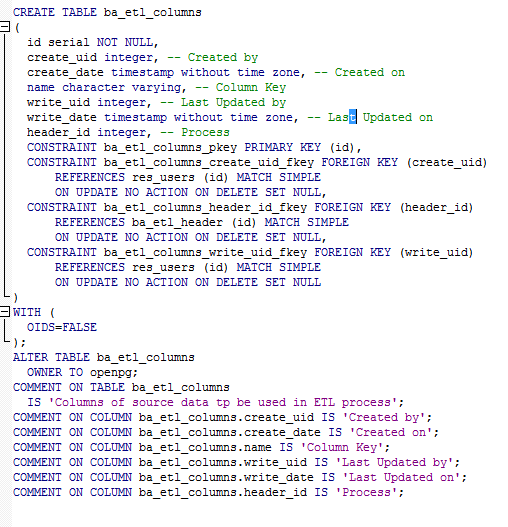
\includegraphics[scale=0.5]{Gambar/tabel-ba-etl-columns}
		\caption{Implementasi tabel ba\_etl\_columns}
		\end{figure}
	
	\item Tabel basisdata ba\_etl\_columns\_mapping\\
	Tabel ini menyimpan detail \textit{mapping} kolom dari data \textit{input} ke \textit{output}.
	\begin{figure}[H]
		\centering
		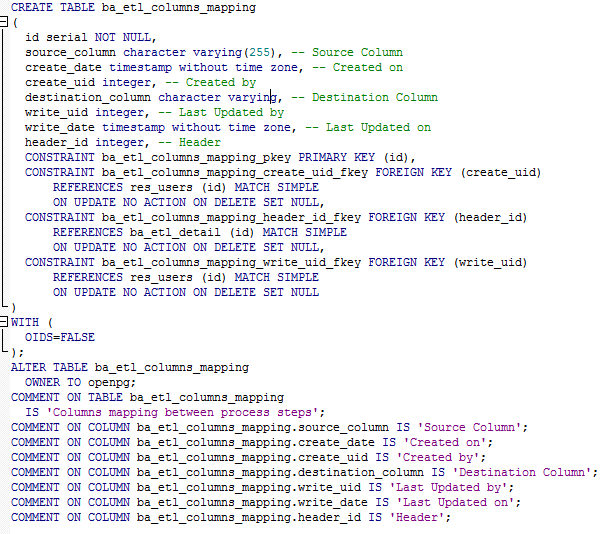
\includegraphics[scale=0.5]{Gambar/tabel-ba-etl-columns-mapping}
		\caption{Implementasi tabel ba\_etl\_columns\_mapping}
		\end{figure}
	
	\item Tabel basisdata ba\_etl\_format\_data\_lines\\ Tabel ini menyimpan detil informasi dari setiap kolom khusus tipe ETL Format Data.
	\begin{figure}[H]
		\centering
		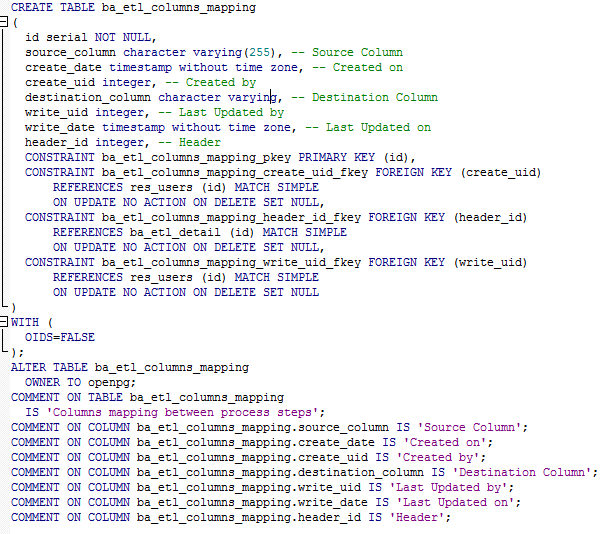
\includegraphics[scale=0.5]{Gambar/tabel-ba-etl-columns-mapping}
		\caption{Implementasi tabel ba\_etl\_columns\_mapping}
		\end{figure}
	
	\item Tabel basisdata ba\_etl\_sort\_data\_columns\\
	Tabel ini menyimpan detail kolom dan arah sorting khusus tipe ETL \textit{Sort Data}
	\begin{figure}[H]
		\centering
		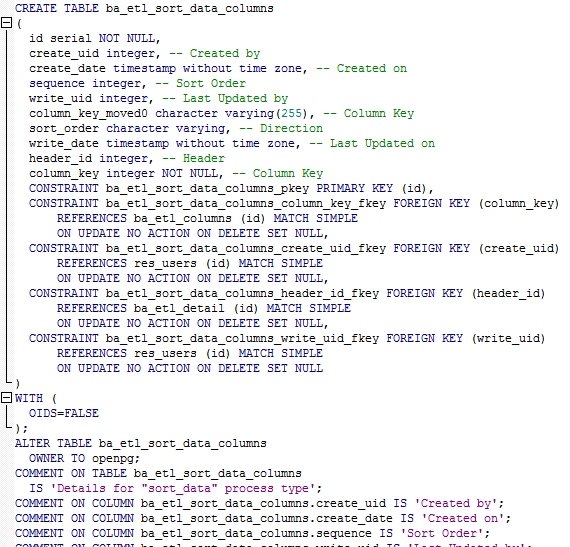
\includegraphics[scale=0.5]{Gambar/tabel-ba-etl-sort-data-columns}
		\caption{Implementasi tabel ba\_etl\_sort\_data\_columns}
		\end{figure}
		
		\item Tabel basisdata ba\_etl\_derived\_column\_lines\\
		Tabel ini menyimpan detail formula untuk menghasilkan \textit{derived column} khusus tipe ETL \textit{Derived Column}.
		\begin{figure}[H]
		\centering
		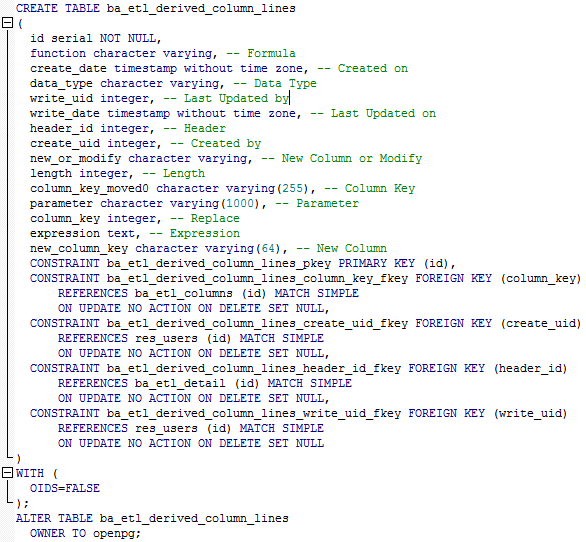
\includegraphics[scale=0.5]{Gambar/tabel-ba-etl-dericed-column-lines}
		\caption{Implementasi tabel ba\_etl\_derived\_column\_lines}
		\end{figure}
		
		\item Tabel basisdata ba\_etl\_lookup\_fixed\_lines\\
		Tabel ini menyimpan pilihan \textit{lookup} yang diambil dari himpan pilihan \textit{fixed}. Khusus tipe ETL \textit{lookup}.
		\begin{figure}[H]
		\centering
		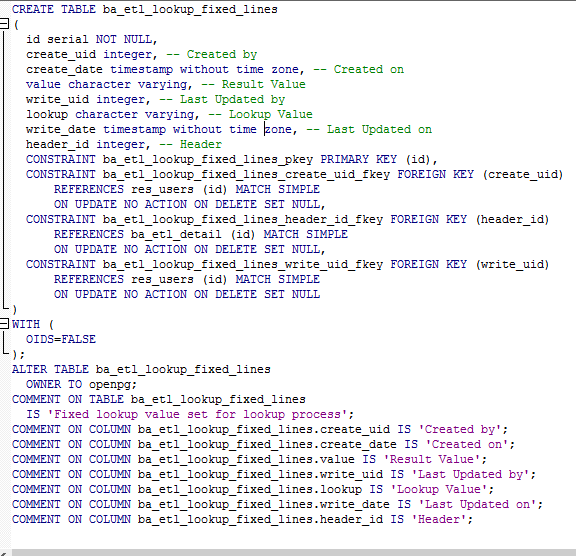
\includegraphics[scale=0.5]{Gambar/tabel-ba-etl-lookup-fixed-lines}
		\caption{Implementasi tabel ba\_etl\_lookup\_fixed\_lines}
		\end{figure}
		
		\item Tabel basisdata ba\_etl\_save\_data\_columns\\
		Tabel ini menyimpan \textit{mapping} kolom antara hasil proses dengan \textit{field} di tabel. Khusus tipe ETL \textit{Save Data} 
		\begin{figure}[H]
		\centering
		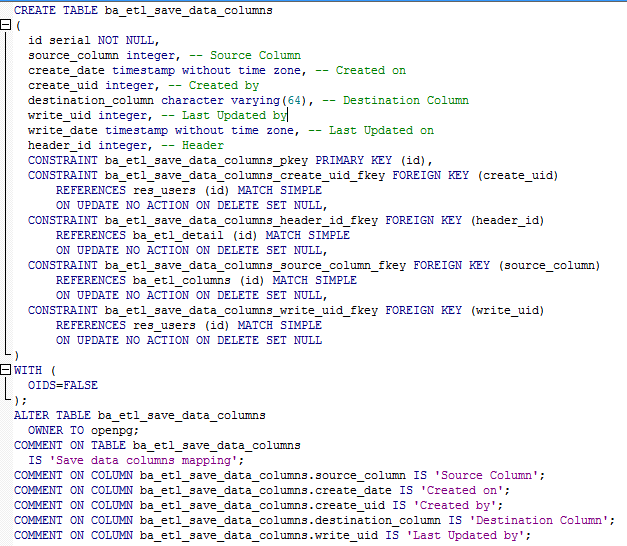
\includegraphics[scale=0.5]{Gambar/tabel-ba-etl-save-data-columns}
		\caption{Implementasi tabel ba\_etl\_save\_data\_columns}
		\end{figure}
		
		\item Tabel basisdata ba\_etl\_lookup\_model\_mappings\\
		Tabel ini menyimpan \textit{lookup} dari tabel lain, tabel ini menampung pasangan \textit{field} di data proses dengan yang di tabel lookup. Khusus tipe ETL \textit{lookup}
		\begin{figure}[H]
		\centering
		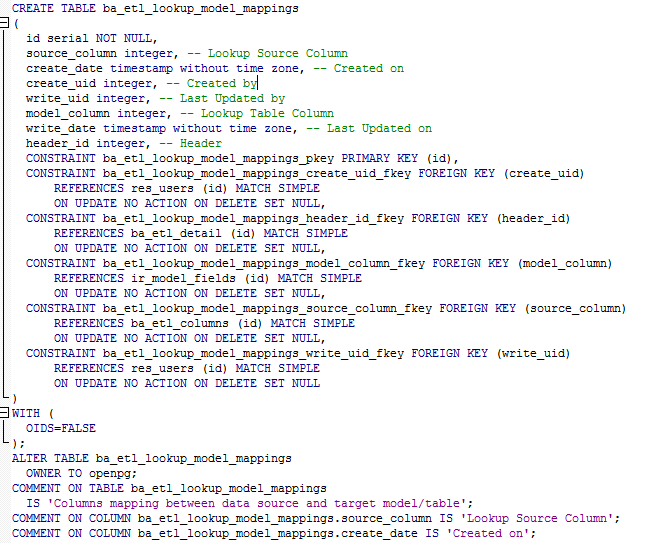
\includegraphics[scale=0.5]{Gambar/tabel-ba-etl-lookup-model-mappings}
		\caption{Implementasi tabel ba\_etl\_lookup\_model\_mappings}
		\end{figure}
		
		\item Tabel basisdata ba\_etl\_merge\_columns1\\
		Tabel ini menyimpan informasi \textit{merge} dari sumber pertama. Khusus tipe ETL \textit{Merge}
		\begin{figure}[H]
		\centering
		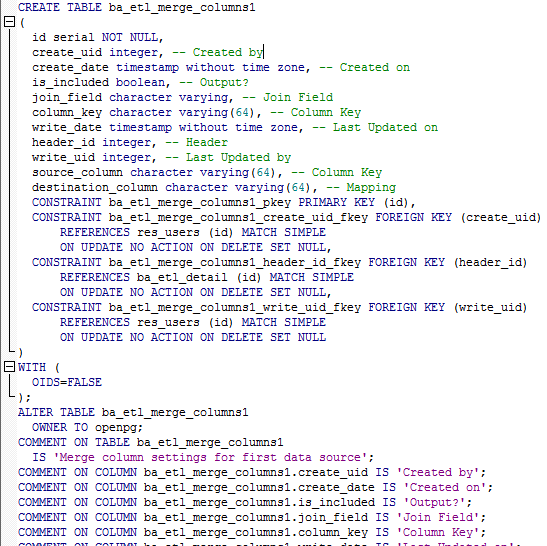
\includegraphics[scale=0.5]{Gambar/tabel-ba-etl-merge-columns1}
		\caption{Implementasi tabel ba\_etl\_merge\_columns1}
		\end{figure}
		
		\item Tabel basisdata ba\_etl\_merge\_columns2\\
		Tabel ini menyimpan informasi \textit{merge} dari sumber kedua. Khusus tipe ETL \textit{Merge}
		\begin{figure}[H]
		\centering
		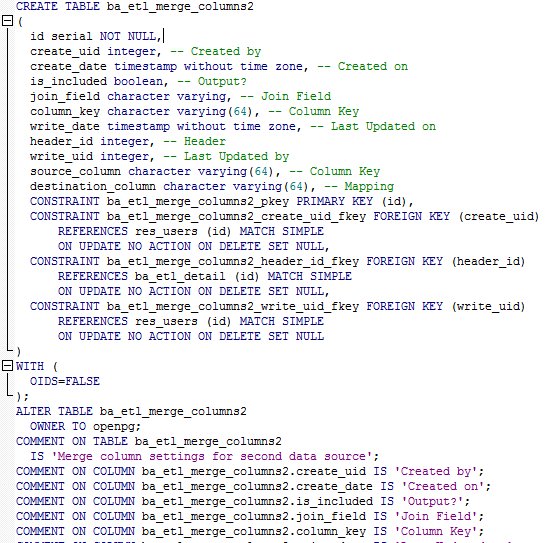
\includegraphics[scale=0.5]{Gambar/tabel-ba-etl-merge-columns2}
		\caption{Implementasi tabel ba\_etl\_merge\_columns2}
		\end{figure}
		
		\item Tabel basisdata ba\_etl\_aggregate\_columns\\
		Tabel ini menyimpan detail informasi proses aggregate khusus tipe ETL \textit{aggregate}.
		\begin{figure}[H]
		\centering
		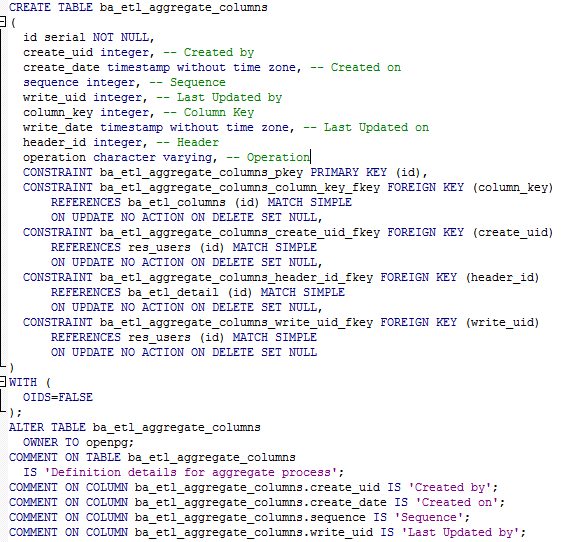
\includegraphics[scale=0.5]{Gambar/tabel-ba-etl-aggregate-columns}
		\caption{Implementasi tabel ba\_etl\_aggregate\_columns}
		\end{figure}
	\end{itemize}
	
	\section{Implementasi Kode Program Phyton}
	Berikut ini sisipan kode program perangkat lunak BI \textit{tool}
	\begin{enumerate}
		\item Kode Program \textit{load} kolom dari \textit{source}\\
		\begin{figure}[H]
		\centering
		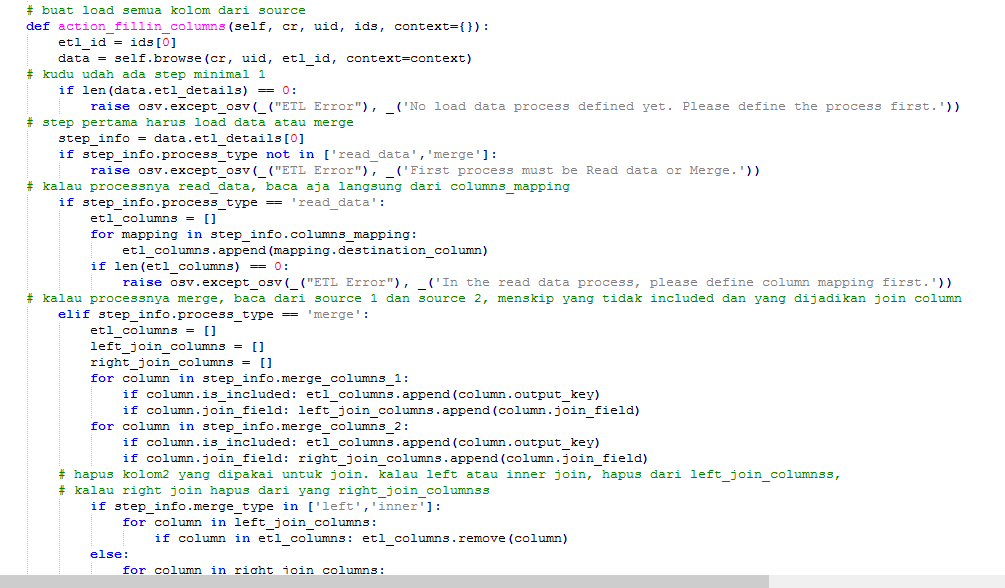
\includegraphics[scale=0.5]{Gambar/kode-load}
		\caption{kode program \textit{load columns from source}}
		\end{figure}
	\item Kode Program untuk \textit{mapping column}
	\begin{figure}[H]
		\centering
		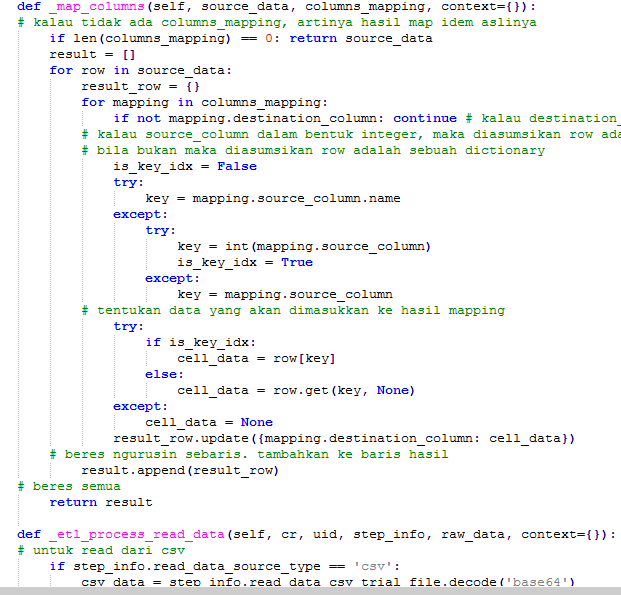
\includegraphics[scale=0.5]{Gambar/kode-mapping}
		\caption{Kode Program untuk \textit{mapping column}}
		\end{figure}
	\end{enumerate}
	
	\section{Implementasi Antar Muka}
	\subsection{Implementasi Antar Muka untuk \textit{Business}}
	\begin{itemize}
		\item Buat Bisnis Baru\\
		Halaman ini digunakan ketika pertama perusahaan akan membuat bisnis baru sebelum masuk pada proses ETL.
		\begin{figure}[H]
		\centering
		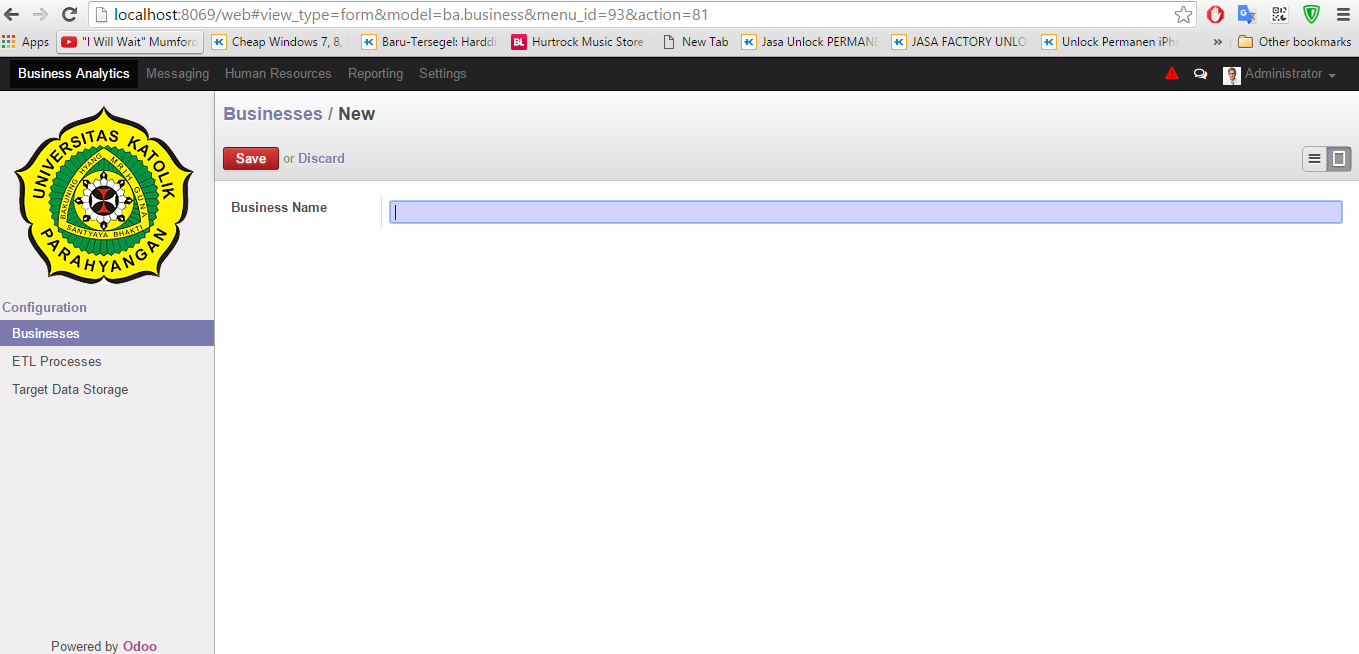
\includegraphics[scale=0.4]{Gambar/tampilan-business}
		\caption{Tampilan untuk membuat bisnis baru}
		\end{figure}
	\end{itemize}
	
	\subsection{Implementasi Antar Muka untuk Proses ETL}
	\begin{itemize}
		\item Membuat Proses ETL Baru\\
		Halaman ini digunakan ketika membuat proses ETL baru.
		\begin{figure}[H]
		\centering
		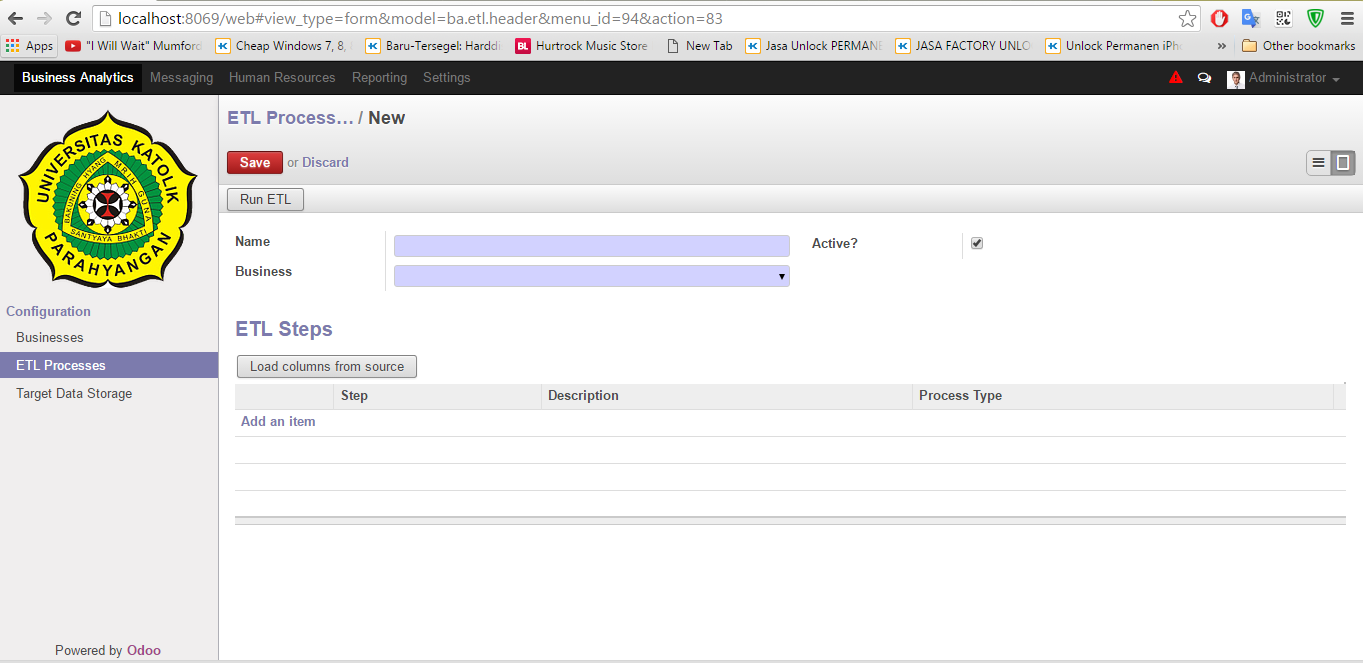
\includegraphics[scale=0.4]{Gambar/tampilan-etl-baru}
		\caption{Tampilan untuk membuat ETL baru}
		\end{figure}
		
		\item \textit{Upload Source}\\
		Halaman ini digunakan ketika pengguna meng-\textit{upload data source}.
		
		\begin{figure}[H]
		\centering
		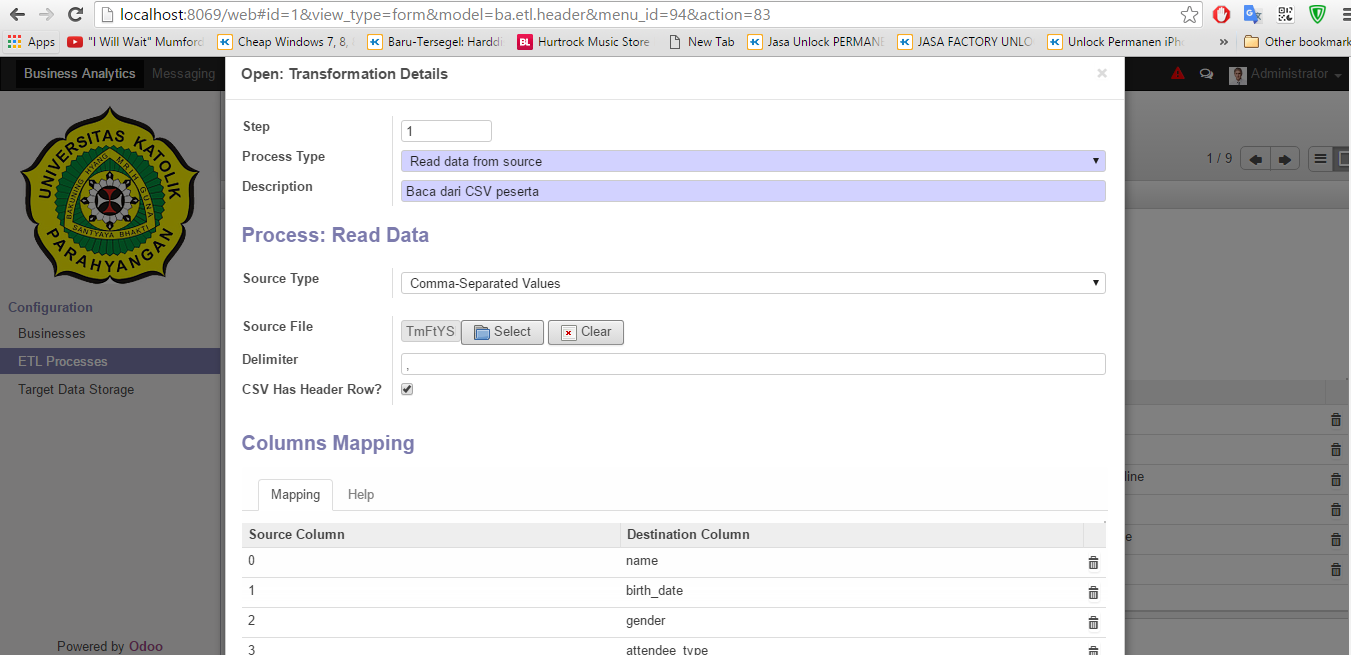
\includegraphics[scale=0.4]{Gambar/tampilan-upload-source}
		\caption{Tampilan untuk \textit{upload source}}
		\end{figure}
		
		\item \textit{Determine Data Types and Format}\\
		Halaman ini memudahkan pengguna untuk menentukan format dan tipe data pada \textit{source}.
		
		\begin{figure}[H]
		\centering
		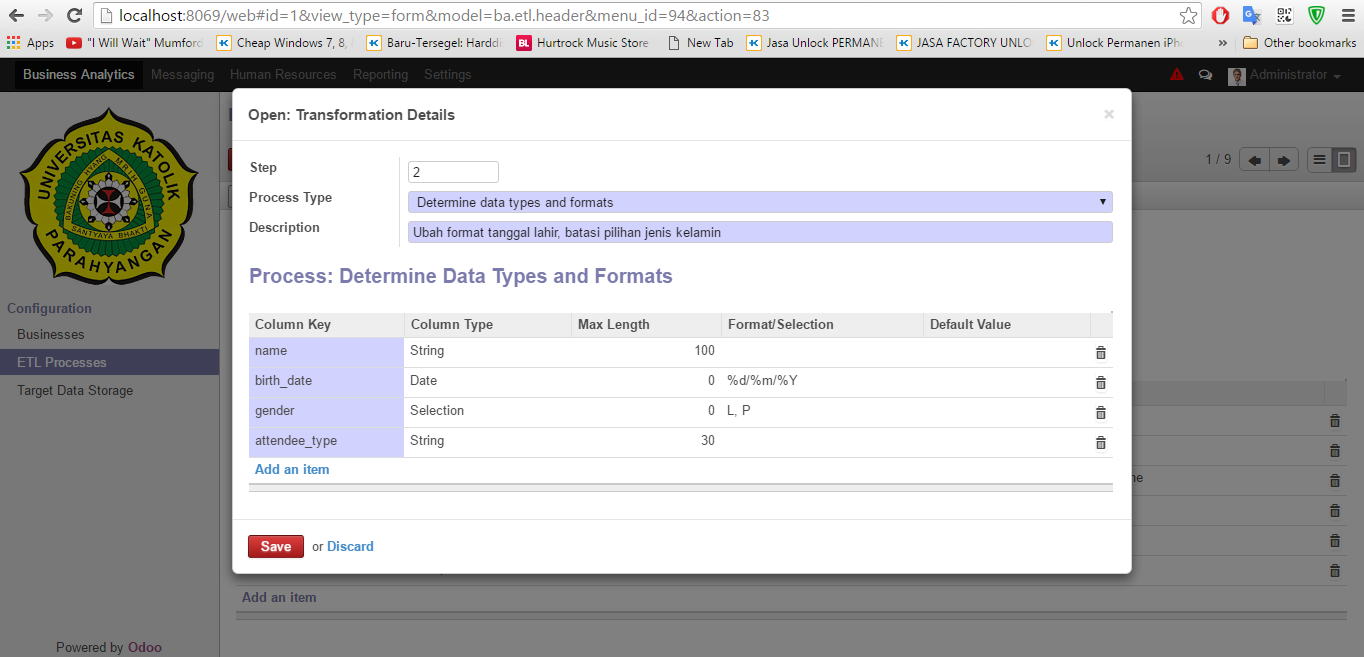
\includegraphics[scale=0.4]{Gambar/tampilan-ubah-data}
		\caption{Tampilan untuk ubah data dan format data}
		\end{figure}
	
	\item Menerapkan Skrip Phyton\\
	Halaman ini dapat digunakan pengguna ketika akan menerapkan kode phyton untuk memodifikasi \textit{source}.
	
	\begin{figure}[H]
		\centering
		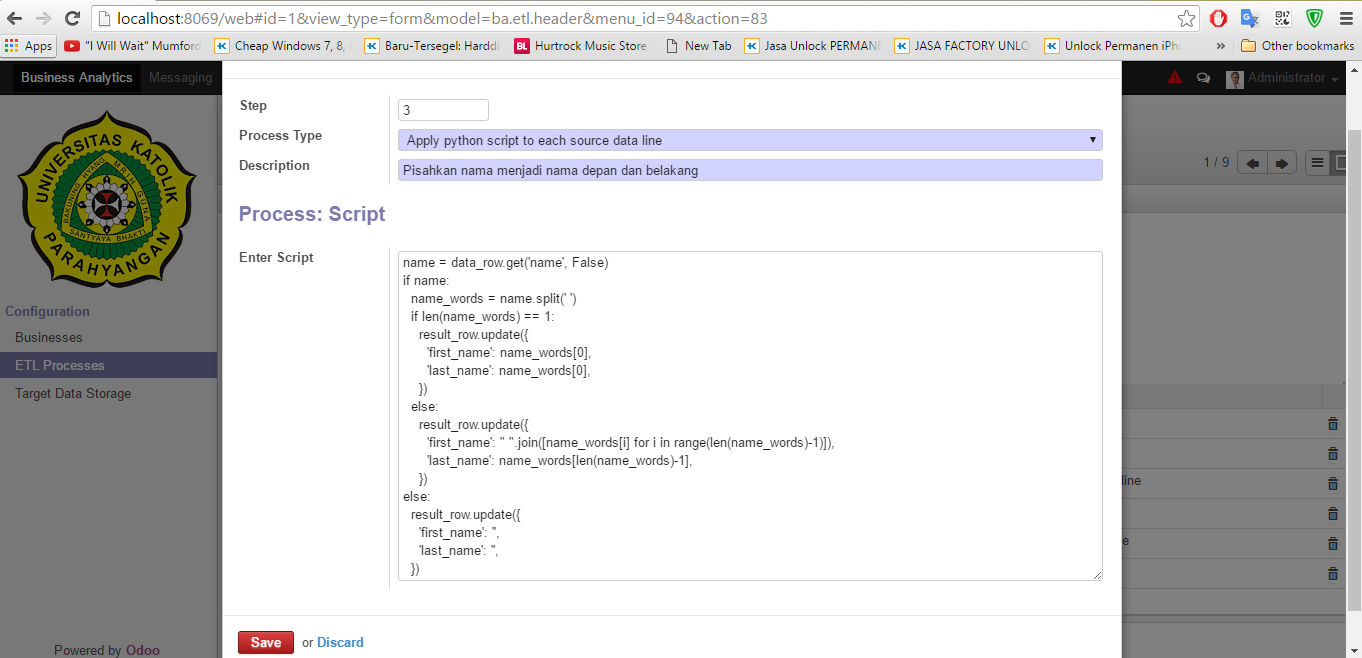
\includegraphics[scale=0.4]{Gambar/tampilan-menerapkan-skrip-phyton}
		\caption{Tampilan untuk menerapkan skrip phyton}
		\end{figure}
		
		\item Tampilan \textit{Lookup} dengan \textit{Existing Table}
		Halaman ini digunakan ketika pengguna ingin melakukan lookup dengan tabel lain yang sudah dimasukan terlebih dahulu dalam \textit{database}
		\begin{figure}[H]
		\centering
		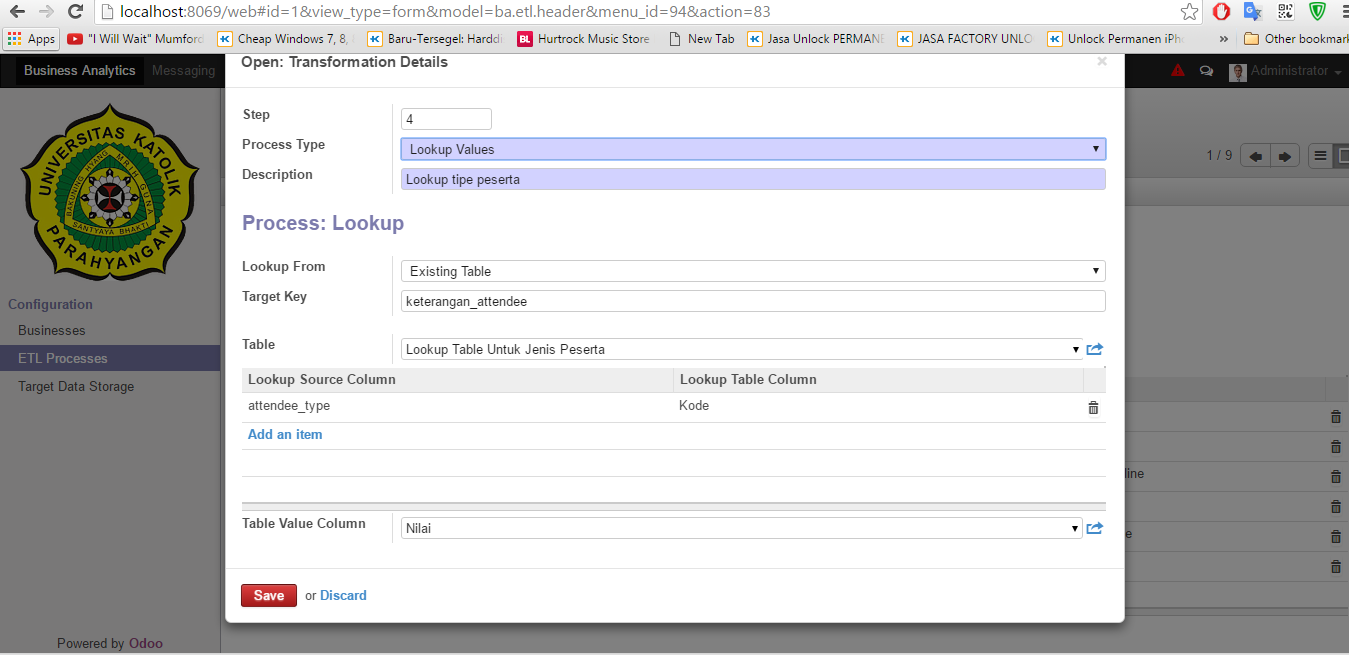
\includegraphics[scale=0.4]{Gambar/tampilan-lookup-existing-table}
		\caption{Tampilan untuk \textit{lookup} dari \textit{existing table}}
		\end{figure}
		
		\item Tampilan \textit{Lookup} dengan \textit{Values Below}
		Halaman ini digunakan ketika pengguna ingin melakukan lookup dengan nilai \textit{lookup} dan hasil yang dimasukan langsung oleh pengguna
		\begin{figure}[H]
		\centering
		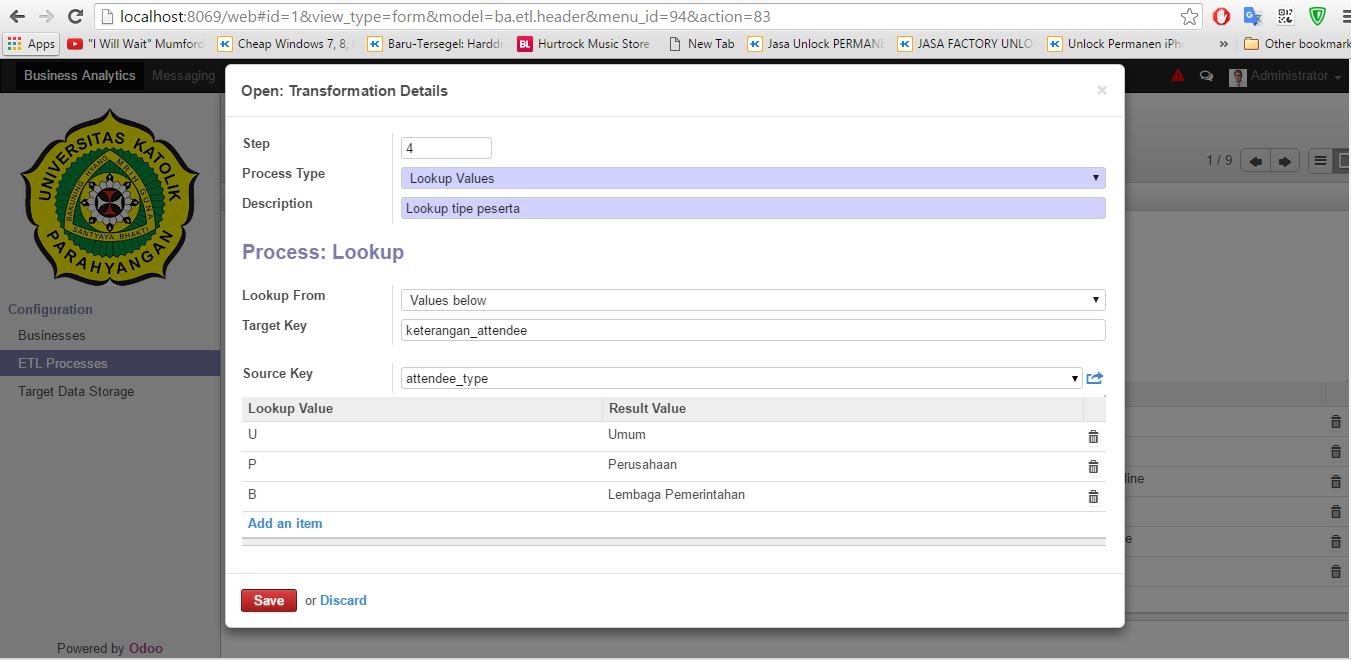
\includegraphics[scale=0.4]{Gambar/tampilan-lookup-values-below}
		\caption{Tampilan untuk \textit{lookup} dari \textit{value} yang dituliskan pengguna}
		\end{figure}
		
		\item Menambah atau memodifikasi kolom yang tersedia\\
		Halaman ini digunakan ketika pengguna ingin menambahkan kolom atau memodifikasi kolom yang tersedia.
		
		\begin{figure}[H]
		\centering
		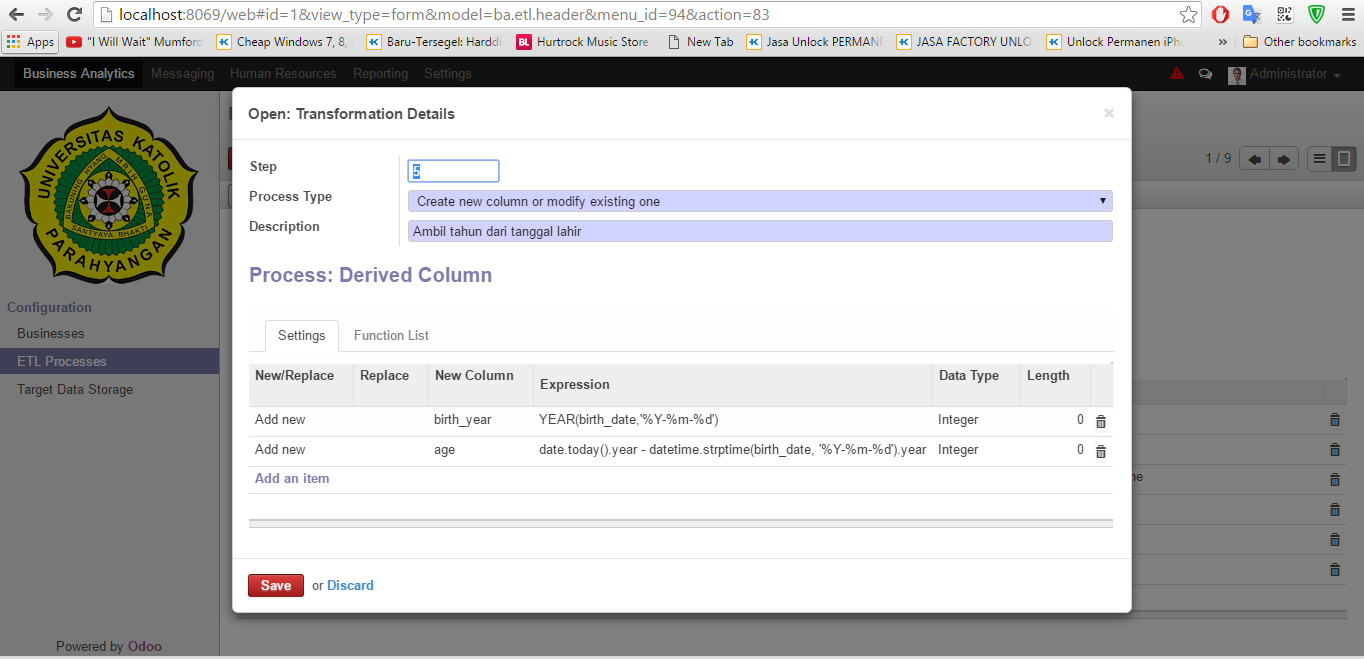
\includegraphics[scale=0.4]{Gambar/tampilan-menambah-kolom}
		\caption{Tampilan untuk menambah atau memodifikasi kolom}
		\end{figure}
		
		
		\item \textit{Merging} dua \textit{data source}\\
		Halaman ini digunakan ketika pengguna ingin menggabungkan dua \textit{data source} menjadi satu.
		
		\begin{figure}[H]
		\centering
		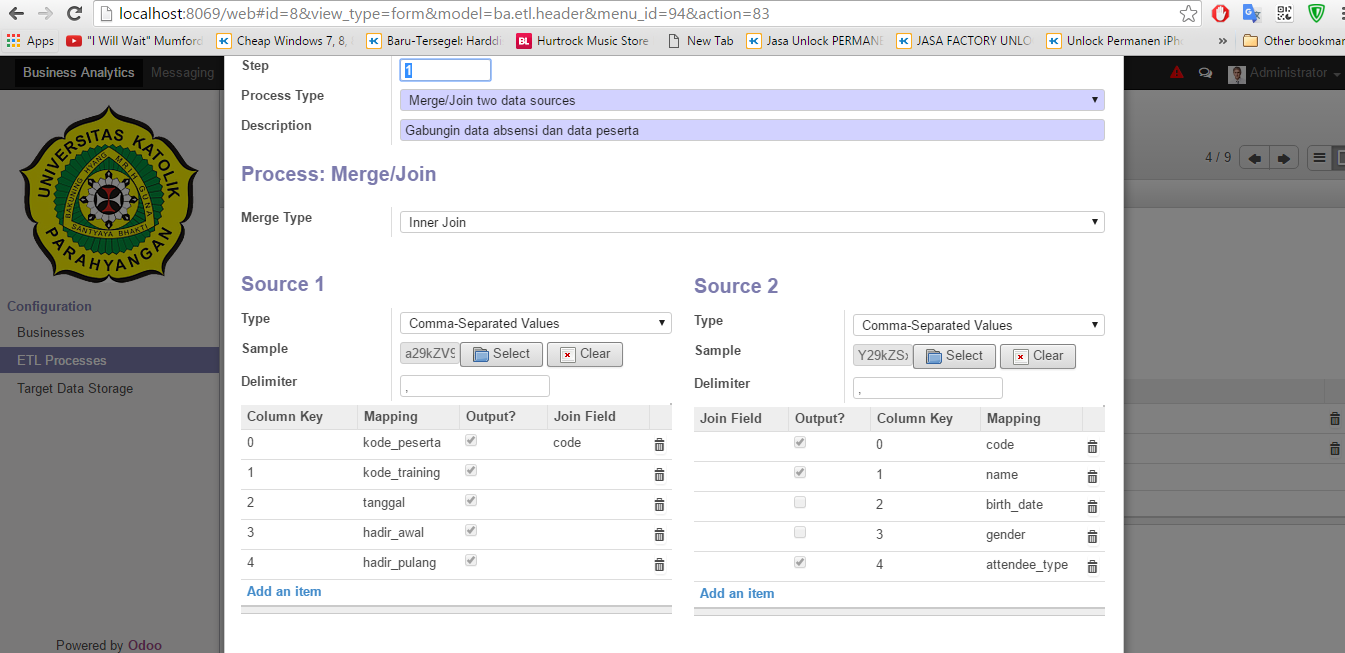
\includegraphics[scale=0.4]{Gambar/tampilan-merge}
		\caption{Tampilan untuk \textit{merging} dua \textit{source}}
		\end{figure}
		
		\item Melakukan \textit{Sorting data}\\
		Halaman ini digunakan ketika pengguna ingin melakukan \textit{sorting data} .
		\begin{figure}[H]
		\centering
		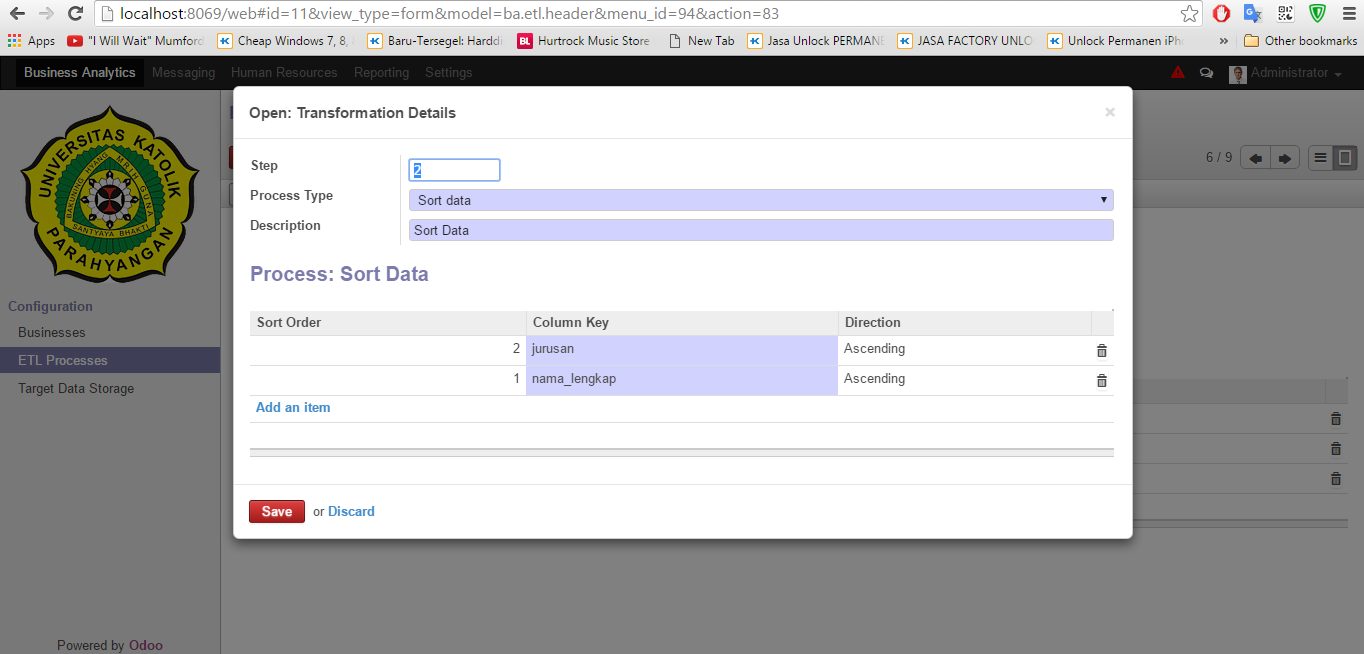
\includegraphics[scale=0.4]{Gambar/tampilan-sort-data}
		\caption{Tampilan untuk melakukan \textit{sort}}
		\end{figure}
		
		\item Melakukan Agregat\\
		Tampilan ini digunakan pengguna ketika akan melakukan agregat terhadap \textit{source}
		\begin{figure}[H]
		\centering
		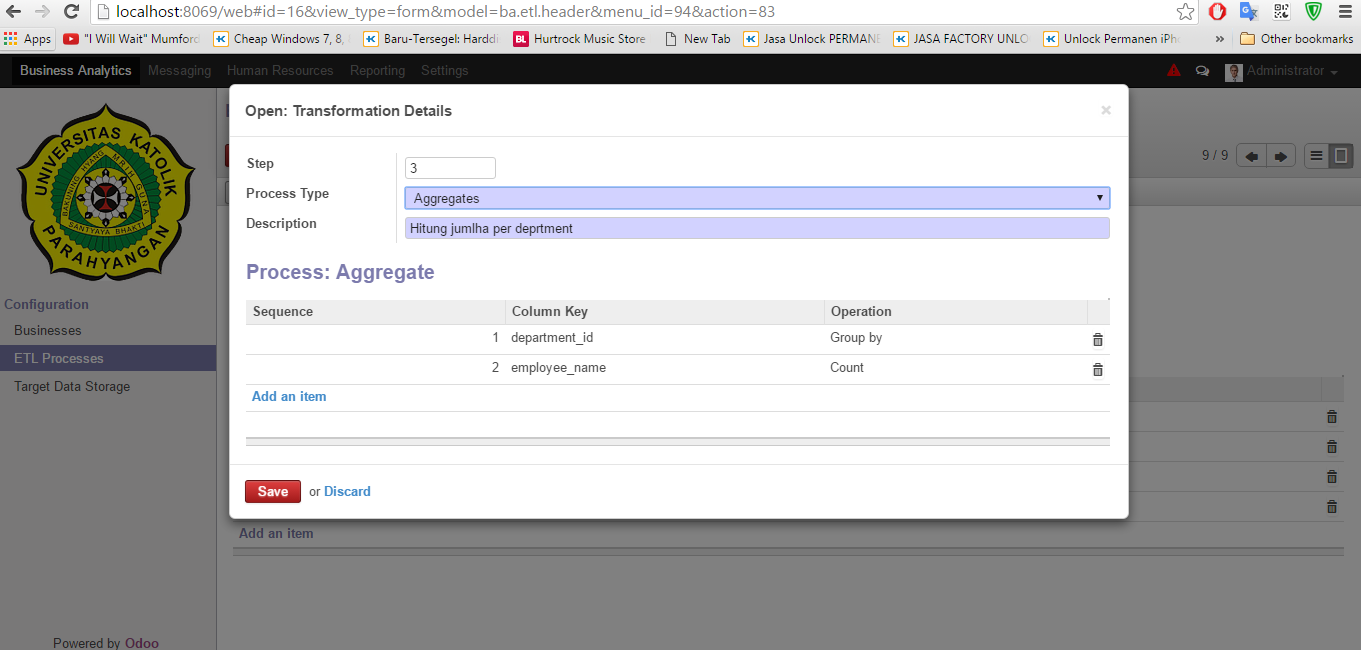
\includegraphics[scale=0.4]{Gambar/tampilan-agregat}
		\caption{Tampilan untuk melakukan agregat}
		\end{figure}
		
		\item Menyimpan ke \textit{database}\\
		Halaman ini digunakan ketika pengguna ingin menyimpan hasil ETL kedalam \textit{database}.

		\begin{figure}[H]
		\centering
		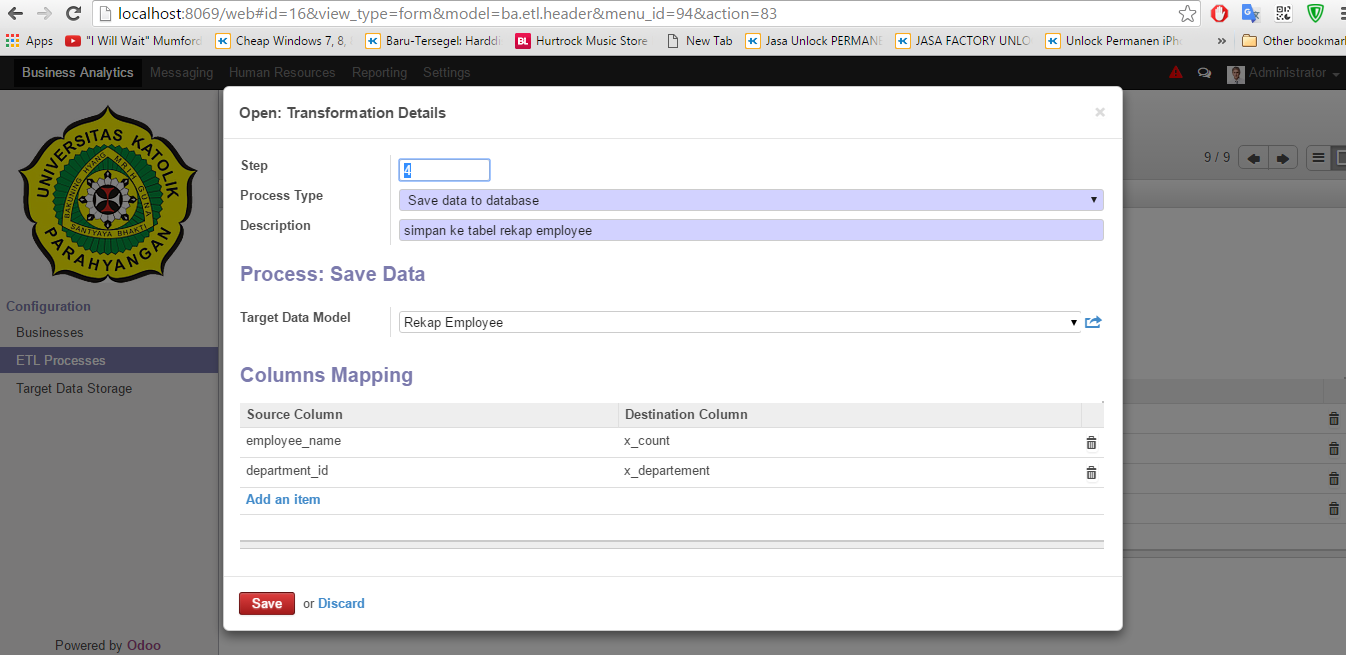
\includegraphics[scale=0.4]{Gambar/tampilan-simpan-database}
		\caption{Tampilan untuk menyimpan kedalam \textit{database}}
		\end{figure}
	\end{itemize}
	
	\section{Pengujian}
	Pada subab ini akan dibahas mengenai pengujian terhadap perangkat lunak ini sehingga dapat mengukur seberapa baik performansinya. berikut ini merupakan \textit{sample data customer} yang akan digunakan.
	
	\begin{table}[H]
	\centering
		\caption{Contoh Tabel \textit{customer}}
		\begin{tabular}{ | c | c| c | c | p{2cm} | p{2cm} | c |}
			\hline
				CIF & BRANCHCODE & GENDER & AGE & MARITAL STATUS & INCOME LEVEL & TENURE \\ \hline \hline
			1000000&ID0010096&2&15131&0&1&1175 \\ \hline 
			1000043&ID0010075&2&14972&1&1&1175 \\ \hline
			1000044&ID0010049&2&13401&1&1&1175 \\ \hline
			1000056&ID0010049&1&18992&1&1&1175 \\ \hline
			1000059&ID0010038&2&20871&1&1&1175 \\ \hline
			1000064&ID0010049&2&20852&1&1&1175 \\ \hline
			1000067&ID0010038&1&15728&1&1&1175 \\ \hline
			1000068&ID0010049&1&16176&1&1&1175 \\ \hline
			1000069&ID0010026&1&19069&1&1&1175 \\ \hline
			1000075&ID0010038&1&11279&1&1&1175 \\ \hline
			1000076&ID0010090&1&18562&1&1&1175 \\ \hline
			1000084&ID0010090&2&14490&1&1&1175 \\ \hline
			1000140&ID0010129&1&15216&1&1&1174 \\ \hline
			1000149&ID0010026&1&9566&0&1&1174 \\ \hline
			1000166&ID0010108&2&14100&1&6&1174 \\ \hline
			1000195&ID0010014&1&12617&0&3&1174 \\ \hline
			1000202&ID0010132&1&23236&1&1&1174 \\ \hline
			1000244&ID0010096&2&19106&1&2&1174 \\ \hline
			1000246&ID0010038&2&27964&1&1&1174 \\ \hline
		\end{tabular}
\end{table}

Hasil Pengujian fitur adalah sebagai berikut.
\begin{enumerate}
	\item \textit{Sort, Aggregate, Modify Existing one, Read Source, Save to Database}\\
	Hasil pengujian proses ETL dapat dilihat pada tabel dibawah ini.
	
	\begin{table}[H]
	\centering
		\caption{Tabel \textit{ba\_bussiness}}
		\begin{tabular}{ | c | p{3cm}| p{3cm}| p{3cm} | }
			\hline
				Hal yang diuji & Hasil yang diharapkan & Hasil Pengujian & Status \\ \hline \hline
			 \textit{Upload CSV} & Berhasil Melakukan \textit{upload} CSV & Berhasil Melakukan \textit{upload} CSV & OK \\ \hline
				Melakukan Sorting & Data tersorting berdasarkan \textit{branchcode} dan \textit{gender}. & Data tersorting berdasarkan \textit{branchcode} dan \textit{gender} & OK \\ \hline
				Melakukan Agregat & Hitung rata-rata umur per cabang per jenis kelamin & Data telah terhitung per rata-rata umur per cabang per jenis kelamin & OK \\ \hline
				Memodifikasi data & Ubah umur ke dalam satuan tahun & Umur telah berhasil diubah kedalam satuan tahun & OK \\ \hline
				Memodifikasi data & Ubah jenis kelamin menjadi P/L & Jenis kelamin menjadi P/L & OK \\ \hline
				Menyimpan ke \textit{database} & Simpan hasil ke \textit{database} & Data berhasil tersimpan ke \textit{database}& OK\\ \hline
			
		\end{tabular}
\end{table}
\end{enumerate}
	
}{}
\ifdefstring{\vbabf}{1}{\chapter{Kesimpulan dan Saran}
\label{chap:Summary}

\section{Kesimpulan}
Setelah melakukan penelitian maka dapat disimpulkan beberapa hal, yakni:
\begin{enumerate}
	\item \textit{Framework} ODOO mendukung untuk pembuatan ETL \textit{tool} yang berperan dalam proses BI.
	\item ODOO bersifat modular sehingga fleksibilitasnya tinggi.
	\item Jika SSIS mebutuhkan 2 \textit{tool} untuk ETL yaitu visual studio dan management studio, ODOO hanya membutuhkan 1 tool saja.
	\item Pengguna tanpa pengetahuan SQL dapat menggunakan \textit{tool} ini.
	
\end{enumerate}

\section{Saran}
Berikut ini saran yang diharapkan dapat membantu pengembangan penelitian ini lebih lanujut, yakni:
\begin{enumerate}
	\item Menambahkan \textit{input data} XML-RPC
	\item Menambahkan OLAP dan Cube
	\item \textit{Merge} yang pada saat ini baru bisa di jalankan apabila ditempatkan paling pertama, diharapkan pada penelitian selanjutnya dapat ditempatkan dimana saja.
\end{enumerate}}{}
\ifdefstring{\vbabg}{1}{\include{Bab/bab7}}{}
\ifdefstring{\vbabh}{1}{\include{Bab/bab8}}{}
\ifdefstring{\vbabi}{1}{\include{Bab/bab9}}{}

\bibliographystyle{ieeetr}
\bibliography{pustaka}

\appendix
\apptoc

\tampillmp{\vlmp}
\ifdefstring{\vlmpa}{1}{\chapter{The Program}
\label{app:A}

The interface of the program is shown in Figure~\ref{fig:appxa2}:

\begin{figure}[H]
\centering
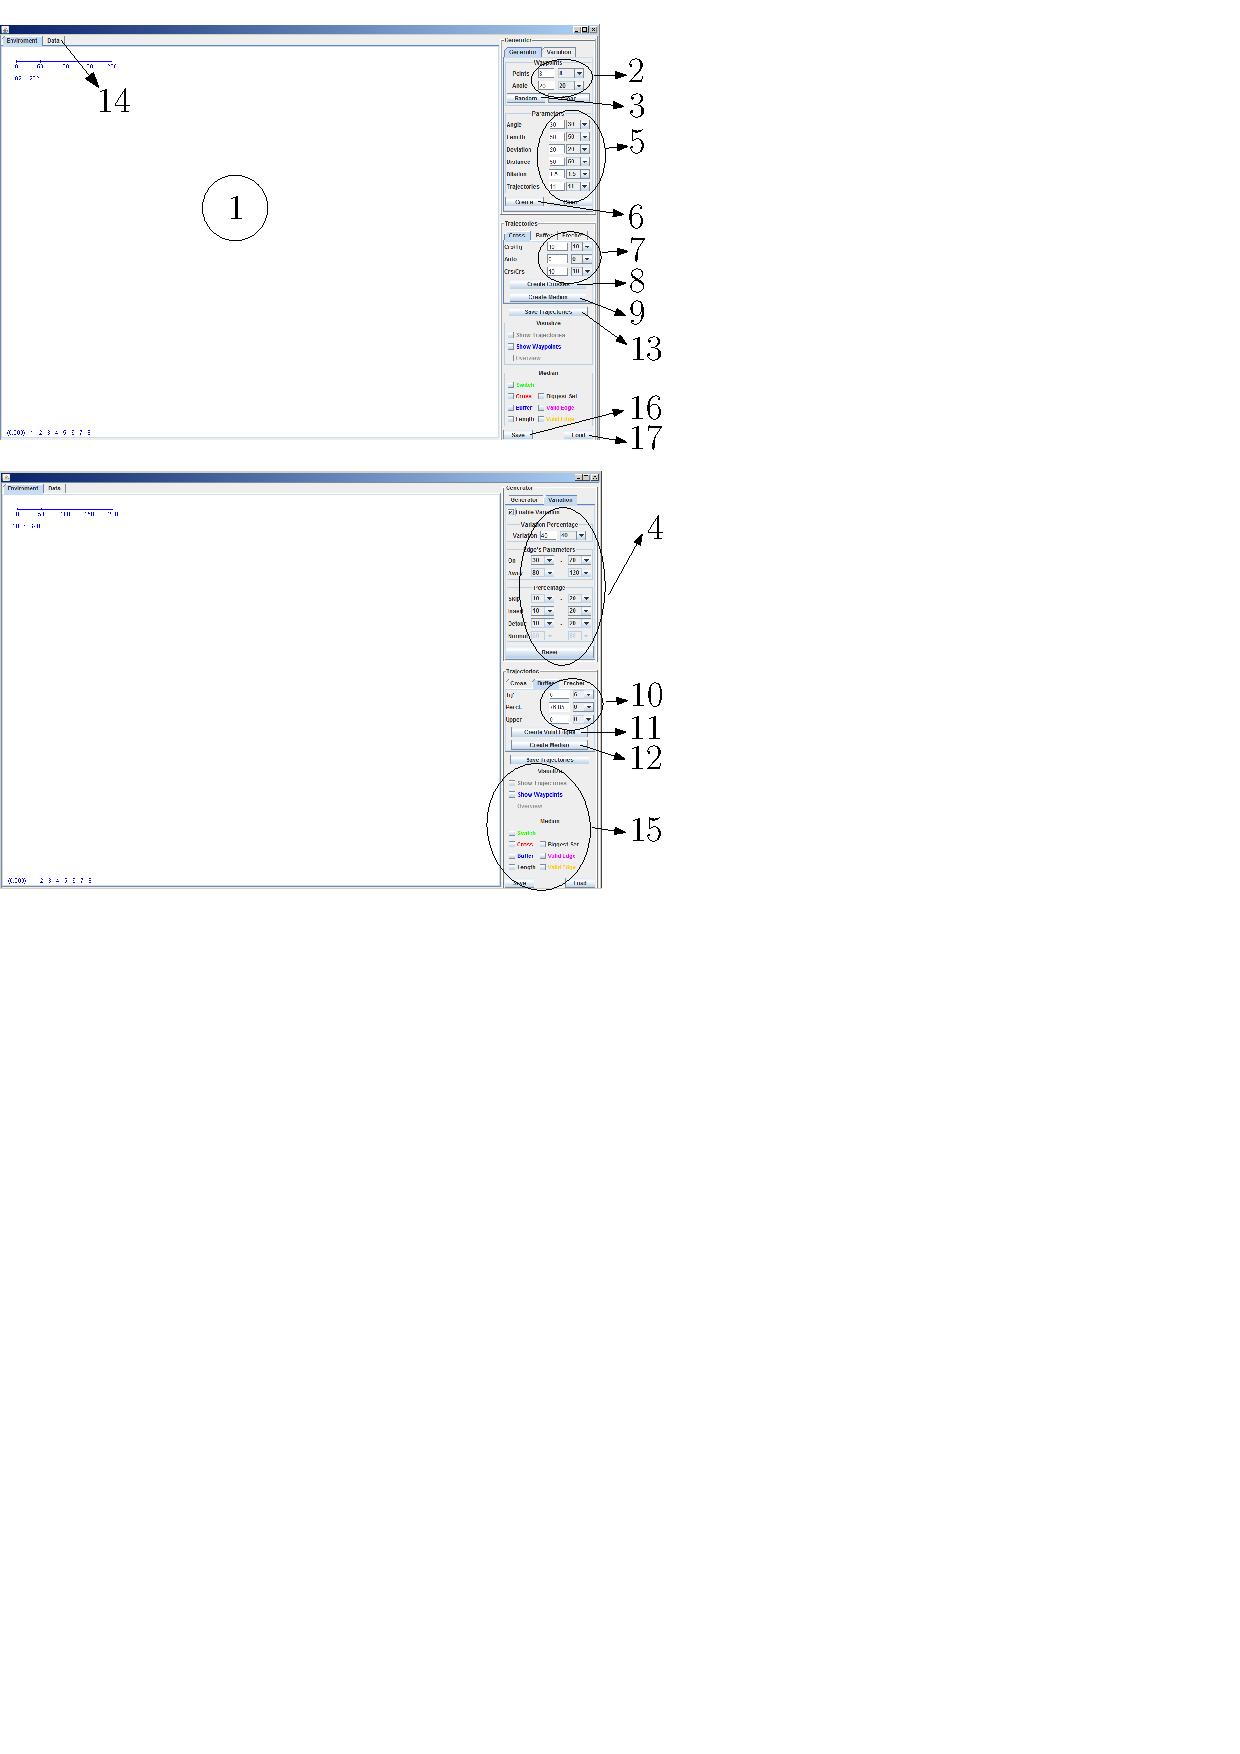
\includegraphics[scale=1]{Gambar/appxa2}
\caption[Interface of the program]{Interface of the program} 
\label{fig:appxa2}
\end{figure}

Step by step to compute the median trajectory using the program:
\begin{enumerate}
\item
Create several waypoints. 
Click anywhere in the ``Environment'' area(1) or create them automatically by setting the parameters for waypoint(2) or clicking the button ``Random''(3).
\item
The ``Variation'' tab could be used to create variations by providing values needed to make them(4).
\item
Create a set of trajectories by setting all parameters(5) and clicking the button ``Create''(6).
\item
Compute the median using the homotopic algorithm: 
\begin{itemize}
\item Define all parameters needed for the homotopic algorithm(7).
\item Create crosses by clicking the ``Create Crosses'' button(8).\item Compute the median by clicking the ``Compute Median'' button(9).
\end{itemize}
\item
Compute the median using the switching method and the buffer algorithm: 
\begin{itemize}
\item Define all parameters needed for the buffer algorithm(10).
\item Create valid edges by clicking the ``Create Valid Edges''button(11). 
\item Compute the median by clicking the ``Compute Median''button(12).
\end{itemize}
\item
Save the resulting median by clicking the ``Save Trajectories'' button(13).
The result is saved in the computer memory and can be seen in ``Data'' tab(14) 
\item 
The set of trajectories and its median trajectories will appear in the ``Environment'' area(1) and the user can change what to display by selecting various choices in ``Visualize'' and ``Median'' area(15).
\item
To save all data to the disk, click the ``Save''(16) button. A file dialog menu will appear.
\item
To load data from the disk, click the ``Load''(17) button.
\end{enumerate}}{}
\ifdefstring{\vlmpb}{1}{\chapter{The Source Code}
\label{app:B}

%selalu gunakan single spacing untuk source code !!!!!
\singlespacing 
% language: bahasa dari kode program
% terdapat beberapa pilihan : Java, C, C++, PHP, Matlab, R, dll
%
% basicstyle : ukuran font untuk kode program
% terdapat beberapa pilihan : tiny, scriptsize, footnotesize, dll
%
% caption : nama yang akan ditampilkan di dokumen akhir, lihat contoh
\begin{lstlisting}[language=Java,basicstyle=\tiny,caption=MyFurSet.java]

import java.util.ArrayList;
import java.util.Collections;
import java.util.HashSet;

/**
 *
 * @author Lionov
 */

//class for set of vertices close to furthest edge
public class MyFurSet {
    protected int id;                                  //id of the set
    protected MyEdge FurthestEdge;                     //the furthest edge
    protected HashSet<MyVertex> set;                   //set of vertices close to furthest edge
    protected ArrayList<ArrayList<Integer>> ordered;   //list of all vertices in the set for each trajectory
    protected ArrayList<Integer> closeID;              //store the ID of all vertices
    protected ArrayList<Double> closeDist;             //store the distance of all vertices
    protected int totaltrj;                            //total trajectories in the set

    /**
     * Constructor
     * @param id : id of the set
     * @param totaltrj : total number of trajectories in the set
     * @param FurthestEdge : the furthest edge
     */
    public MyFurSet(int id,int totaltrj,MyEdge FurthestEdge) {
        this.id = id;
        this.totaltrj = totaltrj;
        this.FurthestEdge = FurthestEdge;
        set = new HashSet<MyVertex>();
        ordered = new ArrayList<ArrayList<Integer>>();
        for (int i=0;i<totaltrj;i++) ordered.add(new ArrayList<Integer>());
        closeID = new ArrayList<Integer>(totaltrj);
        closeDist = new ArrayList<Double>(totaltrj);
        for (int i = 0;i <totaltrj;i++) {
            closeID.add(-1);
            closeDist.add(Double.MAX_VALUE);
        }
    }

    /**
     * set a vertex into the set
     * @param v : vertex to be added to the set
     */
    public void add(MyVertex v) {
        set.add(v);
    }

    /**
     * check whether vertex v is a member of the set
     * @param v : vertex to be checked
     * @return true if v is a member of the set, false otherwise
     */
    public boolean contains(MyVertex v) {
        return this.set.contains(v);
    }
}
\end{lstlisting}}{}
\ifdefstring{\vlmpc}{1}{\chapter{The Source Code}
\label{app:C}

%selalu gunakan single spacing untuk source code !!!!!
\singlespacing 
% language: bahasa dari kode program
% terdapat beberapa pilihan : Java, C, C++, PHP, Matlab, R, dll
%
% basicstyle : ukuran font untuk kode program
% terdapat beberapa pilihan : tiny, scriptsize, footnotesize, dll
%
% caption : nama yang akan ditampilkan di dokumen akhir, lihat contoh
\begin{lstlisting}[language=Java,basicstyle=\tiny,caption=MyFurSet.java]

import java.util.ArrayList;
import java.util.Collections;
import java.util.HashSet;

/**
 *
 * @author Lionov
 */

//class for set of vertices close to furthest edge
public class MyFurSet {
    protected int id;                                  //id of the set
    protected MyEdge FurthestEdge;                     //the furthest edge
    protected HashSet<MyVertex> set;                   //set of vertices close to furthest edge
    protected ArrayList<ArrayList<Integer>> ordered;   //list of all vertices in the set for each trajectory
    protected ArrayList<Integer> closeID;              //store the ID of all vertices
    protected ArrayList<Double> closeDist;             //store the distance of all vertices
    protected int totaltrj;                            //total trajectories in the set

    /**
     * Constructor
     * @param id : id of the set
     * @param totaltrj : total number of trajectories in the set
     * @param FurthestEdge : the furthest edge
     */
    public MyFurSet(int id,int totaltrj,MyEdge FurthestEdge) {
        this.id = id;
        this.totaltrj = totaltrj;
        this.FurthestEdge = FurthestEdge;
        set = new HashSet<MyVertex>();
        ordered = new ArrayList<ArrayList<Integer>>();
        for (int i=0;i<totaltrj;i++) ordered.add(new ArrayList<Integer>());
        closeID = new ArrayList<Integer>(totaltrj);
        closeDist = new ArrayList<Double>(totaltrj);
        for (int i = 0;i <totaltrj;i++) {
            closeID.add(-1);
            closeDist.add(Double.MAX_VALUE);
        }
    }

    /**
     * set a vertex into the set
     * @param v : vertex to be added to the set
     */
    public void add(MyVertex v) {
        set.add(v);
    }

    /**
     * check whether vertex v is a member of the set
     * @param v : vertex to be checked
     * @return true if v is a member of the set, false otherwise
     */
    public boolean contains(MyVertex v) {
        return this.set.contains(v);
    }

    /**
     *  create a column for table Gamma, sorted for each row
     */
    public void createColumn() {
        for (MyVertex v : set) {
            for (Integer key : v.vertexnum.keySet()) {
                for (Integer values : v.vertexnum.get(key)) {
                    ordered.get(key).add(values);
                }
            }
        }
        for (ArrayList<Integer> al : ordered) Collections.sort(al);
    }


}
\end{lstlisting}}{}
\ifdefstring{\vlmpd}{1}{\include{Lampiran/lampD}}{}
\ifdefstring{\vlmpe}{1}{\include{Lampiran/lampE}}{}
\ifdefstring{\vlmpf}{1}{\include{Lampiran/lampF}}{}
\ifdefstring{\vlmpg}{1}{\include{Lampiran/lampG}}{}
\ifdefstring{\vlmph}{1}{\include{Lampiran/lampH}}{}
\ifdefstring{\vlmpi}{1}{\include{Lampiran/lampI}}{}

\end{document}
